\documentclass[aos]{imsart}
 
 
 
\usepackage{xr}
\externaldocument{symcrt-manuscript-aos}
 
%% Packages
\RequirePackage{amsthm,amsmath,amsfonts,amssymb,mathtools,bm,bbm,mathrsfs,soul}  % typesetting
\RequirePackage[authoryear]{natbib}                                         % author-year citations
\RequirePackage[colorlinks,citecolor=blue,urlcolor=blue]{hyperref}          % coloring bibliography citations and linked URLs
\RequirePackage{graphicx}                                                   % figures
\RequirePackage{xcolor}													    % colors
\RequirePackage{caption} 											        % for figure and table captions
\RequirePackage{verbatim}
\RequirePackage[ruled, linesnumbered]{algorithm2e} 					        % for algorithm box
\RequirePackage{subcaption} 					                            % for sub-figure plots

 
 \renewcommand{\theequation}{S\arabic{equation}}
% \renewcommand{\thefigure}{S\arabic{figure}}

 
 \startlocaldefs
 
 
 
 \newcommand{\tikzcircle}[2][red,fill=red]{\tikz[baseline=-0.5ex]\draw[#1,radius=#2] (0,0) circle ;}
 
 
 
 \newcommand{\indmeh}{
 	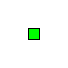
\begin{tikzpicture}
 	\filldraw[fill=green,draw=black] rectangle ++(4pt,4pt);
 	\end{tikzpicture}
 }
 \newcommand{\ind}{
 	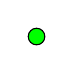
\begin{tikzpicture}
 	\filldraw[fill=green,draw=black] circle (3pt);
 	\end{tikzpicture}
 }
 \newcommand{\posmeh}{
 	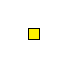
\begin{tikzpicture}
 	\filldraw[fill=yellow,draw=black] rectangle ++(4pt,4pt);
 	\end{tikzpicture}
 }
 \newcommand{\pos}{
 	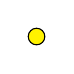
\begin{tikzpicture}
 	\filldraw[fill=yellow,draw=black] circle (3pt);
 	\end{tikzpicture}
 }
 \newcommand{\arbit}{
 	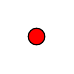
\begin{tikzpicture}
 	\filldraw[fill=red,draw=black] circle (3pt);
 	\end{tikzpicture}
 }
 \newcommand{\arbitmeh}{
 	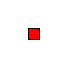
\begin{tikzpicture}
 	\filldraw[fill=red,draw=black] rectangle ++(4pt,4pt);
 	\end{tikzpicture}
 }
 
 
 %\setlength{\parindent}{10pt}
 %\setlength{\parskip}{5pt}
 
 
 %----------------------------------------------------------
 % Theorem etc macros
 %----------------------------------------------------------
 \newtheorem{theorem}{Theorem}
 
 \definecolor{verylightblue}{rgb}{0.7,0.8,1}
 \newenvironment{ftheorem}%
 {\begin{mdframed}[backgroundcolor=verylightblue]\begin{theorem}}%
 		{\end{theorem}\end{mdframed}}
 
 \definecolor{verylightgray}{gray}{0.95}
 \newenvironment{fproof}%
 {\begin{mdframed}[backgroundcolor=verylightgray]\begin{proof}}%
 		{\end{proof}\end{mdframed}}
 
 
 \newtheorem{claim}{Claim}
 \newtheorem{lemma}{Lemma}
 \definecolor{verylightred}{rgb}{1,0.8,0.8}
 \newenvironment{flemma}%
 {\begin{mdframed}[backgroundcolor=verylightred]\begin{lemma}}%
 		{\end{lemma}\end{mdframed}}
 
 
 \newtheorem{proposition}{Proposition}
 \newenvironment{fproposition}%
 {\begin{mdframed}[backgroundcolor=verylightblue]\begin{proposition}}%
 		{\end{proposition}\end{mdframed}}
 
 \newtheorem{corollary}{Corollary}
 \newtheorem{question}{Question}
 \newtheorem{assumption}{Assumption}
 \theoremstyle{definition}
 \newtheorem{definition}{Definition}
 \theoremstyle{remark}
 \newtheorem{remark}{Remark}
 \newtheorem{example}{Example}
 \makeatletter
 
 \newtheorem*{rep@theorem}{\rep@title}
 \newcommand{\newreptheorem}[2]
 {\newenvironment{rep#1}[1]
 	{\def\rep@title{#2 \ref{##1}} \begin{rep@theorem}}%
 		{\end{rep@theorem}}}
 \makeatother
 \newreptheorem{theorem}{Theorem}
 \newreptheorem{lemma}{Lemma}
 \newreptheorem{corollary}{Corollary}
 \newreptheorem{proposition}{Proposition}
 
 
%----------------------------------------------------------
% Generic macros
%----------------------------------------------------------
\newcommand{\E}{\mathbb E}								% expectation
\newcommand{\V}{\mathrm{Var}}							% variance
\renewcommand{\P}{\mathbb{P}}							% probability
\newcommand{\Q}{\mathbb{Q}}								% quantile
\newcommand{\R}{\mathbb{R}}								% reals
\newcommand{\Z}{\mathbb{Z}}								% integers
\newcommand{\indicator}{\mathbbm 1}						% indicator
\newcommand{\norm}[1]{\left\lVert{#1}\right\rVert}		% norm
\newcommand{\independent}{{\perp \! \! \! \perp}}		% independent
\newcommand{\iidsim}{\stackrel{\mathrm{i.i.d.}}{\sim}} 	% i.i.d. distributed
\newcommand{\indsim}{\stackrel{\mathrm{ind}}{\sim}}		% independently distributed
\newcommand{\expit}{\mathrm{expit}}                 	% link function for logistic model
\newcommand{\convp}{\overset p \rightarrow}             % convergence in probability
\newcommand{\convd}{\overset d \rightarrow}             % convergence in distribution
\newcommand{\convas}{\overset {a.s.} \rightarrow}       % convergence almost surely
\newcommand{\argmin}[1]{\underset{#1}{\arg \min}}       % arg min
\newcommand{\argmax}[1]{\underset{#1}{\arg \max}}       % arg max

%----------------------------------------------------------
% Paper-specific macros
%----------------------------------------------------------
\newcommand{\prx}{\bm X}								% population random X
\newcommand{\srx}{X}									% sample random X
\newcommand{\prz}{\bm Z}								% population random Z
\newcommand{\srz}{Z}									% sample random Z 
\newcommand{\prxk}{{{\widetilde{\bm X}}}}      			% population random resampled X
\newcommand{\seta}{s^{2}(\eta_0)}
\newcommand{\srxk}{\widetilde X}						% sample random resampled X
\newcommand{\pry}{{\bm Y}}								% population random Y
\newcommand{\sry}{Y}									% sample random Y 
\newcommand{\peps}{\bm \epsilon}						% population epsilon
\newcommand{\seps}{\epsilon}							% sample epsilon
\newcommand{\smu}{\mu}									% sample mu
\newcommand{\pmu}{\bm \mu}								% population mu
\newcommand{\law}{\mathcal L}							% law of (X,Y,Z)
\newcommand{\nulllaws}{\mathscr L^0}					% collection of null distributions
\newcommand{\regclass}{\mathscr R}					    % collection of distributions with regularity
\newcommand{\lawhat}{\widehat{\mathcal L}}				% estimated law of (X,Y,Z)
\newcommand{\CRT}{\textnormal{CRT}}             		% CRT
\newcommand{\dCRT}{\textnormal{dCRT}} 					% dCRT
\newcommand{\GCM}{\textnormal{GCM}}						% GCM
\newcommand{\dCRThat}{\widehat{\textnormal{dCRT}}}		% dCRT-hat
\newcommand{\MXtwohat}{\widehat{\textnormal{MX(2)}}}	% dCRT-hat
\newcommand{\ndCRThat}{\widehat{\textnormal{ndCRT}}}	% normalized dCRT-hat
\newcommand{\CRThat}{\widehat{\textnormal{CRT}}}		% CRT-hat
\renewcommand{\H}{\mathcal H}		 					% Hilbert subspace
\newcommand{\MXtwo}{\textnormal{MX(2)}}                 % MX(2)
\newcommand{\convdp}{\overset {d,p} \longrightarrow}    % conditional convergence in distribution
\newcommand{\convpp}{\overset {p,p} \longrightarrow}    % conditional convergence in probability
\newcommand{\old}[1]{{\color{red}{#1}}}
\newcommand{\nav}[1]{{\color{blue}{#1}}}
\newcommand{\zn}[1]{{\color{blue}{#1}}}
\definecolor{darkgreen}{rgb}{0.0, 0.5, 0.0}
\newcommand{\new}[1]{{\color{darkgreen}{#1}}}

%----------------------------------------------------------
% Other macros
%----------------------------------------------------------
\let\oldnl\nl% Store \nl in \oldnl
\newcommand{\nonl}{\renewcommand{\nl}{\let\nl\oldnl}} % Remove line number for one line of alg

% \renewcommand{\thefootnote}{\fnsymbol{footnote}}

\endlocaldefs



\begin{document}


\begin{frontmatter}
	\title{{Supplement to: \\ ``Reconciling model-X and doubly robust approaches\\ 
	to conditional independence testing''}}
	\runtitle{Model-X and doubly robust conditional independence testing}

	\begin{aug}
		%%%%%%%%%%%%%%%%%%%%%%%%%%%%%%%%%%%%%%%%%%%%%%%
		%% Only one address is permitted per author. %%
		%% Only division, organization and e-mail is %%
		%% included in the address.                  %%
		%% Additional information can be included in %%
		%% the Acknowledgments section if necessary. %%
		%% ORCID can be inserted by command:         %%
		%% \orcid{0000-0000-0000-0000}               %%
		%%%%%%%%%%%%%%%%%%%%%%%%%%%%%%%%%%%%%%%%%%%%%%%
		\author[A]{\fnms{Ziang}~\snm{Niu$^*$}\ead[label=e1]{ziangniu@wharton.upenn.edu}},
		\author[A]{\fnms{Abhinav}~\snm{Chakraborty$^*$}\ead[label=e2]{abch@wharton.upenn.edu}},
		\author[B]{\fnms{Oliver}~\snm{Dukes}\ead[label=e3]{oliver.dukes@ugent.be}}
		\and
		\author[A]{\fnms{Eugene}~\snm{Katsevich}\ead[label=e4]{ekatsevi@wharton.upenn.edu}}
		%%%%%%%%%%%%%%%%%%%%%%%%%%%%%%%%%%%%%%%%%%%%%%
		%% Addresses                                %%
		%%%%%%%%%%%%%%%%%%%%%%%%%%%%%%%%%%%%%%%%%%%%%%
		\address[A]{Department of Statistics and Data Science, University of Pennsylvania \printead[presep={,\ }]{e1,e2,e4}}
		
		\address[B]{Department of Applied Mathematics, Computer Science and Statistics, Ghent University\printead[presep={,\ }]{e3}}
		\end{aug}
	\end{frontmatter}


% %%%%%%%%%%%%%%%%%%%%%%%%%%%%%%%%%%%%%%%%%%%%%%
% %% Multiple Appendixes:                     %%
% %%%%%%%%%%%%%%%%%%%%%%%%%%%%%%%%%%%%%%%%%%%%%%
\appendix

\section{The $\dCRThat$ with GCM normalization} \label{sec:ndcrt}

As an alternative to the $\dCRThat$, we consider the $\ndCRThat$. This procedure is based on a normalized statistic that coincides exactly with the GCM statistic:
\begin{equation*}
T^{\ndCRThat}_n(\srx,\sry,\srz) \equiv \frac{1}{\widehat S_{n}^{\GCM}}T_n^{\dCRThat}(\srx, \sry, \srz) \equiv T^{\GCM}_n(\srx, \sry, \srz).
\end{equation*}
The only difference with GCM is that the critical value is given by conditional resampling rather than a normal quantile:
\begin{equation}
	\begin{split}
		\phi^{\ndCRThat}_n(\srx, \sry, \srz) &\equiv \indicator(T_n^{\ndCRThat}(\srx, \sry, \srz) > \Q_{1-\alpha}[T_n^{\ndCRThat}(\srxk, \srx, \sry, \srz) \mid \srx, \sry, \srz]) \\
		&\equiv \indicator\left(T_n^{\ndCRThat}(\srx, \sry, \srz) > C^{\ndCRThat}_n(\srx, \sry, \srz)\right).
	\end{split}
\end{equation}
Here, 
\begin{equation*}
T_n^{\ndCRThat}(\srxk, \srx, \sry, \srz) \equiv \frac{T_n^{\dCRT}(\srxk, \srx, \sry, \srz)}{S_n^{\GCM}(\srxk, \srx, \sry, \srz)},
\end{equation*}
where 
\begin{equation*}
(S_n^{\GCM}(\srxk, \srx, \sry, \srz))^2 \equiv \widehat{\V}\{(\srxk_i - \widehat \mu_{n,x}(\srz_i))(\sry_i - \widehat \mu_{n,y}(\srz_i))\}
\end{equation*}
and $T_n^{\dCRT}(\srxk, \srx, \sry, \srz)$ is as defined in equation~\eqref{eq:resampled-dcrt-def}.

\begin{theorem}\label{thm:normal-limit-ndcrt} 
	Let $\law_n$ be a sequence of laws such that the nondegeneracy conditions~\eqref{eq:var-bounded-below} and~\eqref{eq:variance-bounds} and the conditional Lyapunov condition~\eqref{eq:lyapunov-condition} hold. Then,
	\begin{equation}
		T^{\ndCRThat}_n(\srxk, \srx, \sry,\srz) \mid \srx, \sry, \srz \convdp N(0,1)
		\label{eq:conditional-convergence-ndcrt}
	\end{equation}
	and therefore
	\begin{equation}
		C^{\ndCRThat}_n(\srx, \sry, \srz) \equiv \Q_{1-\alpha}\left[T^{\ndCRThat}_n(\srxk, \srx, \sry,\srz) \mid \srx, \sry, \srz\right] \rightarrow z_{1-\alpha}
		\label{eq:critical-value-convergence-ndcrt}
	\end{equation}
	and the $\ndCRThat$ and GCM tests are equivalent:
	\begin{equation}
	\lim_{n \rightarrow \infty} \P_{\law_n}[\phi_n^{\ndCRThat}(\srx, \sry, \srz) = \phi_n^{\GCM}(\srx, \sry, \srz)] = 1.
	\label{eq:ndcrt-gcm-equivalence}
	\end{equation}
\end{theorem}

\begin{corollary}
\label{cor:double-robustness-ndcrt}
Let $\regclass_n$ be a sequence of regularity conditions such that for any sequence $\law_n \in \regclass_n$, we have the the nondegeneracy conditions~\eqref{eq:var-bounded-below} and~\eqref{eq:variance-bounds}, the conditional Lyapunov condition~\eqref{eq:lyapunov-condition}, and the assumptions~\eqref{eq:sp1} and~\eqref{eq:sp2}. Then, the $\ndCRThat$ has asymptotic Type-I error control over $\nulllaws_n \cap \regclass_n$ in the sense of the definition~\eqref{eq:asymptotic-control}.
\end{corollary}
Comparing Corollary~\ref{cor:double-robustness-ndcrt} to Corollary~\ref{cor:dcrt-double-robustness}, we see that the $\ndCRThat$ controls Type-I error under weaker assumptions than required for the $\dCRThat$; in particular the variance of $\law_n(\prx|\prz)$ need not be estimated with any degree of accuracy.


\section{Conditional convergence results} \label{sec:conditional-convergence-results}

The proofs of our theoretical results rely on the conditional counterparts of several standard convergence theorems. In this section, we state these conditional convergence theorems. We defer their proofs to Appendix~\ref{sec:conditional-convergence-proofs}.

First we define a notion of conditional convergence in probability, analogous to our definition of conditional convergence in distribution (Definition~\ref{def:conditional-convergence-distribution}).

\begin{definition} \label{def:conditional-convergence-probability}
	For each $n$, let $W_n$ be a random variable and let $\mathcal F_n$ be a $\sigma$-algebra. Then, we say $W_n$ converges in probability to a constant $c$ conditionally on $\mathcal F_n$ if $W_n$ converges in distribution to the delta mass at $c$ conditionally on $\mathcal F_n$ (recall Definition~\ref{def:conditional-convergence-distribution}). We denote this convergence by ${W_n \mid \mathcal F_n \convpp c}$. In symbols, 
	\begin{equation}
		W_n \mid \mathcal F_n \convpp c \quad \text{if} \quad W_n \mid \mathcal F_n \convdp \delta_c.
	\end{equation}
\end{definition}

\noindent Now we are ready to state the conditional convergence results. 

\subsection{Statements}

For the sake of all results below, let $\mathcal F_n$ be a sequence of $\sigma$-algebras.

\begin{theorem}[Conditional Polya's theorem]\label{thm:cond_polya} 
	Let $W_n$ be a sequence of random variables. If $W_n \mid \mathcal F_n \convdp W$ for some random variable $W$ with continuous CDF, then
	\begin{equation}
		\sup_{t \in \R}|\P[W_n \leq t \mid \mathcal F_n] - \P[W \leq t]| \convp 0.
	\end{equation}

\end{theorem}

\begin{theorem}[Conditional Slutsky's theorem]\label{thm:cond_slutsky}
	Let $W_n$ be a sequence of random variables. Suppose $a_n$ and $b_n$ are sequences of random variables such that $a_n \convp 1$ and $b_n \convp 0$. If $W_n \mid \mathcal F_n \convdp W$ for some random variable $W$ with continuous CDF, then
	\begin{equation}
		a_n W_n + b_n \mid \mathcal F_n \convdp W.
	\end{equation}
	
\end{theorem}

\begin{theorem}[Conditional law of large numbers]\label{thm:wlln_cond} 
	Let $W_{in}$ be a triangular array of random variables, such that $W_{in}$ are independent conditionally on $\mathcal F_n$ for each $n$. If for some $\delta > 0$ we have
	\begin{equation}
		\frac{1}{n^{1+\delta}}\sum_{i=1}^n\E[|W_{in}|^{1+\delta}\mid\mathcal{F}_n] \convp 0,
		\label{eq:wlln_cond_assumption}
	\end{equation}
	then 
	\begin{equation}
		\frac{1}{n} \sum_{i = 1}^n (W_{in} - \E[W_{in}|\mathcal{F}_n]) \mid \mathcal F_n \convpp 0.
		\label{eq:wlln_cond_conclusion}
	\end{equation}
	The condition~\eqref{eq:wlln_cond_assumption} is satisfied when
	\begin{equation}
		\sup_{1\leq i\leq n}\E[|W_{in}|^{1+\delta} \mid \mathcal{F}_n]=o_p(n^{\delta}).
		\label{eq:wlln_cond_sufficient}
	\end{equation}
\end{theorem}

As a corollary of Theorem~\ref{thm:wlln_cond}, if we choose $\mathcal{F}_n=\{\varnothing,\Omega\}$, we are able to obtain the following version of the weak law of large numbers for triangular arrays.

\begin{corollary}[Unconditional weak law of large numbers] \label{cor:wlln} 
	Let $W_{in}$ be a triangular array of random variables, such that $W_{in}$ are independent for each $n$. If for some $\delta > 0$ we have
	\begin{equation}
		\frac{1}{n^{1+\delta}}\sum_{i=1}^n\E[|W_{in}|^{1+\delta}] \rightarrow 0,
		\label{eq:one-plus-delta-moment-condition}
	\end{equation}
	then 
	\begin{equation}
		\frac{1}{n} \sum_{i = 1}^n (W_{in} - \E[W_{in}]) \convp 0.
	\end{equation}
	The condition~\eqref{eq:one-plus-delta-moment-condition} is satisfied when
	\begin{equation}
		\sup_{1\leq i\leq n}\E[|W_{in}|^{1+\delta}]=o(n^{\delta}).
		\label{eq:wlln_sufficient}
	\end{equation}
\end{corollary}


\begin{theorem}[Conditional central limit theorem] \label{thm:conditional-clt} 
	Let $W_{in}$ be a triangular array of random variables, such that for each $n,W_{in}$ are independent conditionally on $\mathcal F_n$. Define
	\begin{equation}
		S_n^2 \equiv \sum_{i = 1}^n \V[W_{in} \mid \mathcal F_n],
	\end{equation} 
	and assume $0 < \mathrm{Var}[W_{in}|\mathcal{F}_n]<\infty $ almost surely for all $i=1,\ldots,n$ and for all $n\in\mathbb{N}$. If for some $\delta > 0$ we have
	\begin{equation}
		\frac{1}{S_n^{2+\delta}} \sum_{i = 1}^n \E[|W_{in}-\E[W_{in}|\mathcal{F}_n]|^{2+\delta} \mid \mathcal{F}_n] \convp 0,
		\label{eq:conditional-lyapunov}
	\end{equation}
	then 
	\begin{equation}
		\frac{1}{S_n} \sum_{i = 1}^n (W_{in} - \E[W_{in} \mid \mathcal{F}_n]) \mid \mathcal F_n \convdp N(0,1).
	\end{equation}
	
\end{theorem}

\begin{lemma}[Conditional convergence implies quantile convergence] \label{lem:conditional-convergence-to-quantile} 
	Let $W_n$ be a sequence of random variables and $\alpha \in (0,1)$. If $W_n \mid \mathcal F_n \convdp W$ for some random variable $W$ whose CDF is continuous and strictly increasing at $\mathbb Q_{\alpha}[W]$, then
	\begin{equation}
		\Q_{\alpha}[W_n \mid \mathcal F_n] \convp \Q_{\alpha}[W].
	\end{equation}
\end{lemma}

\subsection{Discussion}

The above definitions and results on conditional convergence are not particularly surprising, and related results are present in the existing literature. Nevertheless, we have not found any of the above results stated in the literature in exactly this form. Here we discuss the relationships of our definitions and results with existing ones.

Notions of conditional convergence in probability and in distribution have been explicitly defined by \citet{Nowak2005}. However, these notions require a single conditioning $\sigma$-algebra as well as almost sure convergences of conditional probabilities, whereas in Definitions~\ref{def:conditional-convergence-distribution} and~\ref{def:conditional-convergence-probability} we allow the conditioning $\sigma$-algebra to change with $n$ and for the conditional probabilities to converge in probability. Our Definition~\ref{def:conditional-convergence-distribution} can be viewed as formalizing the notion of conditional convergence in distribution implicitly used by \citet{Wang2020b}. Related notions of conditional convergence in distribution allowing for changing conditioning $\sigma$-algebra are present implicitly in the works of \citet{Dedecker2002} and \citet{bulinski2017conditional}, though these are based on the convergence of conditional characteristic functions as opposed to conditional cumulative distribution functions. % We prove in Lemma~\ref{lem:concf_to_weak} that in-probability convergence of conditional characteristic functions \citep{bulinski2017conditional} implies in-probability convergence of conditional cumulative distribution functions (Definition~\ref{def:conditional-convergence-distribution}).

Turning to the convergence results themselves, we were not able to find conditional Polya's theorem (Theorem~\ref{thm:cond_polya}) in the literature. Conditional Slutsky's theorem (Theorem~\ref{thm:cond_slutsky}) is a generalization of \citet[Lemma 5]{Wang2020b} to the case when $a_n$ is not necessarily independent of $\mathcal F_n$ and $b_n \neq 0$. Versions of the conditional law of large numbers are given by \cite{Majerek2005a} and \cite{PrakasaRao2009}, but these involve a single conditioning $\sigma$-algebra and do not allow for triangular arrays, unlike Theorem~\ref{thm:wlln_cond}. Remarkably, we could not find even the unconditional triangular array law of large numbers (Corollary~\ref{cor:wlln}) in the literature; existing results either assume a second-moment condition or use truncation \citep[Theorems 2.2.4 and 2.2.6, respectively]{Durrett2010} instead of a $1+\delta$ moment condition or are not applicable to triangular arrays \citep[Lemma 19]{Shah2018}. As for central limit theorems, \citet{Grzenda2008, PrakasaRao2009, Yuan2014} give non-triangular array versions of the conditional central limit theorem that require a single conditioning $\sigma$-algebra, unlike Theorem~\ref{thm:conditional-clt}. Versions of the conditional central limit theorem appropriate for varying conditioning $\sigma$-algebras and triangular arrays are given by \citet{Dedecker2002, bulinski2017conditional}, those these involve different notions of conditional convergence in distribution. Results similar to Theorem~\ref{thm:conditional-clt} for $\delta = 1$ are presented in a recent line of work on sample-splitting-based inference \citep{Kim2020a, Shekhar2022a, Shekhar2022}; these can be proved via the Berry-Esseen theorem. Finally, we note that our result that conditional convergence in distribution implies in-probability quantile convergence (Lemma~\ref{lem:conditional-convergence-to-quantile}) is a generalization of \citet[Lemma 3]{Wang2020b} to general conditioning $\sigma$-algebras.

\section{Proofs for Section~\ref{sec:conv-to-normal}}

\subsection{Auxiliary lemmas}

\begin{lemma}
	\label{lem:conditional-expectation-to-unconditional}
	Let $W_n$ be a sequence of nonnegative random variables and let $\mathcal F_n$ be a sequence of $\sigma$-algebras. If $\E[W_n \mid \mathcal{F}_n]\convp 0$, then $ W_n \convp 0$.
\end{lemma}
\begin{proof}
	For any $\epsilon>0$, we have
	\begin{align}
		\P[W_n \geq \epsilon] &= \P[W_n \wedge \epsilon \geq \epsilon] \\
		&\leq \epsilon^{-1} \E[W_n \wedge \epsilon] \\
		&= \epsilon^{-1} \E[\E[W_n \wedge \epsilon\mid \mathcal{F}_n]]\\
		&\leq \epsilon^{-1} \E[\E[W_n \mid \mathcal{F}_n]\wedge \epsilon] \to 0,
	\end{align}
	where the last convergence is due to bounded convergence theorem and the assumption $\E[W_n \mid \mathcal{F}_n]\convp 0$. 
\end{proof}


\begin{lemma}[Asymptotic equivalence of tests] \label{lem:equivalence-lemma}
	
	Consider two hypothesis tests based on the same test statistic $T_n(\srx, \sry, \srz)$ but different critical values:
	\begin{equation*}
		\phi_n^1(\srx, \sry, \srz) \equiv \indicator(T_n(\srx, \sry, \srz) > C_n(\srx, \sry, \srz)); \quad \phi_n^2(\srx, \sry, \srz) \equiv \indicator(T_n(\srx, \sry, \srz) > z_{1-\alpha}). 
	\end{equation*}
	If the critical value of the first converges in probability to that of the second:
	\begin{equation}
		C_n(\srx, \sry, \srz) \convp z_{1-\alpha}
		\label{eq:convergence-of-critical-value}
	\end{equation}
	and the test statistic does not accumulate near the limiting critical value:
	\begin{equation}
		\lim_{\delta \rightarrow 0}\limsup_{n \rightarrow \infty}\ \P_{\law_n}[|T_n(\srx, \sry, \srz)-z_{1-\alpha}| \leq \delta] = 0,
		\label{eq:non-accumulation-app}
	\end{equation}
	then the two tests are asymptotically equivalent:
	\begin{equation}
		\lim_{n \rightarrow \infty}\P_{\law_n}[\phi_n^{1}(\srx, \sry, \srz) = \phi_n^2(\srx, \sry, \srz)] = 1.
	\end{equation}
\end{lemma}

\begin{proof}
	
	Note that for any $\delta>0$, we have
	\begin{equation}
		\begin{aligned}
			\mathbb{P}_{\law_{n}}&  {\left[\phi_{n}^{1}(\srx,\sry,\srz) \neq \phi_{n}^{2}(\srx,\sry,\srz)\right] } \\
			&= \mathbb{P}_{\law_{n}}\left[\min \left(z_{1-\alpha}, C_{n}\right)<T_{n} \leq \max \left(z_{ 1-\alpha}, C_{n}\right)\right] \\
			&= \mathbb{P}_{\law_{n}}\left[\min \left(z_{ 1-\alpha}, C_{n} \right)<T_{n} \leq \max \left(z_{ 1-\alpha}, C_{n}\right),\left|C_{n}-z_{ 1-\alpha}\right| \leq \delta\right] \\
			&\quad+\mathbb{P}_{\law_{n}}\left[\min \left(z_{ 1-\alpha}, C_{n}\right)<T_{n} \leq \max \left(z_{ 1-\alpha}, C_{n}\right),\left|C_{n}-z_{ 1-\alpha}\right|>\delta\right] \\
			& \leq  \mathbb{P}_{\law_{n}}\left[\left|T_{n}-z_{1-\alpha}\right| \leq \delta\right]+\mathbb{P}_{\law_{n}}\left[\left|C_{n}-z_{ 1-\alpha}\right|>\delta\right] .
		\end{aligned}
		\label{eq:tests-not-same}
	\end{equation}
	
	\noindent To justify the last step, suppose without loss of generality that $z_{1-\alpha} \leq C_n$. Then note that if $z_{1-\alpha}<T_{n} \leq C_{n}$ and $C_{n}-z_{1-\alpha} \leq \delta$ then
	$$
	|T_{n} - z_{1-\alpha}| = T_{n} -z_{1-\alpha} \leq C_n-z_{1-\alpha} \leq \delta.
	$$
	Taking a limsup on both sides in equation~\eqref{eq:tests-not-same} and using the assumed convergence~\eqref{eq:convergence-of-critical-value}, we find that
	$$
	\begin{aligned}
		\limsup_{n\to \infty}\mathbb{P}_{\law_{n}} & {\left[\phi_{n}^{1}(\srx,\sry,\srz) \neq \phi_{n}^{2}(\srx,\sry,\srz)\right] } \\
		\leq & \limsup_{n\to \infty}\mathbb{P}_{\law_{n}}\left[\left|T_{n}(\srx,\sry,\srz)-z_{1-\alpha}\right| \leq \delta\right]+ \limsup_{n\to \infty}\mathbb{P}_{\law_{n}}\left[\left|C_{n}(\srx,\sry,\srz)-z_{ 1-\alpha}\right|>\delta\right]\\
		= &\limsup_{n\to \infty}\mathbb{P}_{\law_{n}}\left[\left|T_{n}(\srx,\sry,\srz)-z_{1-\alpha}\right| \leq \delta\right].
	\end{aligned}
	$$
	Letting $\delta \rightarrow 0$ and using our assumption~\eqref{eq:non-accumulation-app}, we arrive at the claimed asymptotic equivalence. This completes the proof.
\end{proof}


\subsection{Proofs of main results}

\begin{proof}[Proofs of Theorem~\ref{thm:normal-limit} and Corollary~\ref{cor:asymptotic-equivalence}] 
We prove instead the stronger Theorem~\ref{thm:normal-limit-stronger} and Corollary~\ref{cor:asymptotic-equivalence-stronger} below.
\end{proof}

\begin{theorem} \label{thm:normal-limit-stronger}
	Let $\law_n$ be a sequence of laws and $\lawhat_n$ be a sequence of estimates. Suppose either of the following two sets of assumptions is satisfied: 
	\begin{enumerate}
		\item The nondegeneracy conditions ~\eqref{eq:var-bounded-below} and~\eqref{eq:variance-bounds} and the conditional Lyapunov condition~\eqref{eq:lyapunov-condition} hold.
		\item The assumptions of Theorem~\ref{thm:equivalence} hold.
	\end{enumerate}
	Then, the normalized $T_n^{\dCRThat}(\srxk, \srx, \sry, \srz)$ converges conditionally to a normal distribution~\eqref{eq:conditional-convergence} and therefore the $\dCRThat$ critical value $C^{\dCRThat}_n(\srx, \sry, \srz)$ converges to $z_{1-\alpha}$~\eqref{eq:critical-value-convergence}.
\end{theorem}

\begin{proof}

It suffices to prove the conditional convergence in distribution~\eqref{eq:conditional-convergence}, as the convergence of the critical value~\eqref{eq:critical-value-convergence} follows from Lemma~\ref{lem:conditional-convergence-to-quantile} because the normal distribution has continuous and strictly increasing CDF. We prove the conditional convergence~\eqref{eq:conditional-convergence} for each of the two sets of assumptions.

\paragraph*{Assumption 1}

We proceed by applying the conditional CLT (Theorem~\ref{thm:conditional-clt}) with 
\begin{equation}
W_{in} \equiv \frac{1}{\sqrt{n}}(\srxk_i - \widehat \mu_{n,x}(\srz_i))(\sry_i - \widehat \mu_{n,y}(\srz_i))
\end{equation}
and $\mathcal F_n \equiv \sigma(\srx, \sry, \srz)$. To verify the assumptions of the conditional CLT, note first that $W_{in}$ are independent conditionally on $\mathcal F_n$ by construction and satisfy $0 < \V[W_{in} \mid \mathcal F_n] < \infty$ by the nondegeneracy assumption~\eqref{eq:variance-bounds}. Next, recalling definition~\eqref{eq:conditional-variance-def}, we have
\begin{equation*}
S^2_n \equiv \sum_{i = 1}^n \V_{\lawhat_n}[W_{in}\mid \srx,\sry,\srz] \equiv (\widehat S_n^{\dCRThat})^2,
\end{equation*}
so that
\begin{align*}
		&\frac{1}{S_n^{2+\delta}} \sum_{i = 1}^n \E_{\lawhat_n}[|W_{in}|^{2+\delta} \mid \srx,\sry,\srz] \\
		&\quad= \frac{1}{(\widehat S_n^{\dCRThat})^{2+\delta}} \cdot \frac{1}{n^{1+\delta/2}} \sum_{i=1}^n |\sry_i-\widehat\mu_{n,y}(\srz_i)|^{2+\delta}\E_{\lawhat_n}\left[\left|\srxk_i-\widehat\mu_{n,x}(\srz_i)\right|^{2+\delta}\mid \srx,\srz\right].
\end{align*}
This quantity converges to zero in probability due to the nondegeneracy condition~\eqref{eq:var-bounded-below} and the Lyapunov condition~\eqref{eq:lyapunov-condition}. Hence, the conditional CLT gives the desired conditional convergence~\eqref{eq:conditional-convergence}.
 
 \paragraph*{Assumption 2}

We begin by decomposing $T_n^{\dCRThat}(\srxk, \srx, \sry, \srz)$:
 \begin{align}
 	T_n^{\dCRThat}(\srxk, \srx, \sry, \srz) &= \frac{1}{\sqrt n} \sum_{i = 1}^n (\srxk_i - \widehat \mu_{n,x}(\srz_i))(\sry_i - \mu_{n,y}(\srz_i)) \\
 	&\quad -\frac{1}{\sqrt n}\sum_{i = 1}^n (\srxk_i - \widehat \mu_{n,x}(\srz_i))(\widehat \mu_{n,y}(\srz_i) - \mu_{n,y}(\srz_i))\\
	&\equiv I_n - J_n.
 \end{align}
We claim that $J_n \convp 0$. Indeed, from $\E[J_n \mid \srx,\sry,\srz] = 0$ and the assumption $\widehat E'_{n, y} \convp 0$~\eqref{eq:sp1prime} it follows
\begin{equation*}
\E[J_n^2 \mid \srx,\sry,\srz] = \V[J_n \mid \srx,\sry,\srz] \equiv (\widehat E'_{n,y})^2 \convp 0. 
\end{equation*}
Hence by Lemma \ref{lem:conditional-expectation-to-unconditional} we have $J_n^2 \convp 0$, so that $J_n \convp 0$, as claimed. Next, we claim that an appropriately rescaled $I_n$ converges conditionally to $N(0,1)$. To this end, we apply the conditional CLT (Theorem~\ref{thm:conditional-clt}) with
 \begin{equation}
 	W_{in} \equiv \frac{1}{\sqrt{n}}(\srxk_i - \widehat \mu_{n,x}(\srz_i))(\sry_i - \mu_{n,y}(\srz_i))
 \end{equation}
 and $\mathcal{F}_n \equiv \sigma(\srx,\sry,\srz)$. To verify the assumptions of the conditional CLT, note first that $W_{in}$ are independent conditionally on $\mathcal F_n$ by construction and satisfy $0 < \V[W_{in} \mid \mathcal F_n] < \infty$ by the nondegeneracy assumption~\eqref{eq:variance-bounds}. Next, observe that
 \begin{equation*}
	S^2_n \equiv \sum_{i = 1}^n \V[W_{in}\mid \srx,\sry,\srz] =  \frac{1}{n}\sum_{i = 1}^n \V_{\lawhat_n}[\srx_i|\srz_i](\sry_i - \mu_{n,y}(\srz_i))^2 \equiv(S_n^{\dCRThat})^2,
 \end{equation*}
so that
\begin{align*}
	&\frac{1}{S_n^{2+\delta}} \sum_{i = 1}^n \E[|W_{in}|^{2+\delta} \mid \srx,\sry,\srz] \\
	&\quad= \frac{1}{(S_n^{\dCRThat})^{2+\delta}} \cdot \frac{1}{n^{1+\delta/2}} \sum_{i=1}^n |\sry_i-\mu_{n,y}(\srz_i)|^{2+\delta}\E_{\lawhat_n}[|\srxk_i-\widehat\mu_{n,x}(\srz_i)|^{2+\delta}\mid \srx,\srz].
\end{align*}
Since the first factor is stochastically bounded (conclusion~\eqref{eq:bounded-away-from-zero} from Lemma~\ref{lem:cond-sample-variance-equivalence2}), it suffices to show that the second factor converges to zero in probability. To this end, by Lemma~\ref{lem:conditional-expectation-to-unconditional} it suffices to note that $\law_n \in \nulllaws_n$ and the Lyapunov assumption~\eqref{eq:lyapunov-condition-2} give
\begin{equation}
\begin{split}
&\E\left[\left.\frac{1}{n^{1+\delta/2}} \sum_{i=1}^n |\sry_i-\mu_{n,y}(\srz_i)|^{2+\delta}\E_{\lawhat_n}[|\srxk_i-\widehat\mu_{n,x}(\srz_i)|^{2+\delta}\mid \srx,\srz] \right| \srx, \srz \right] \\
&\quad= \frac{1}{n^{1+\delta/2}} \sum_{i=1}^n \E_{\law_n}[|\sry_i-\mu_{n,y}(\srz_i)|^{2+\delta}|\srz_i]\E_{\lawhat_n}[|\srxk_i-\widehat\mu_{n,x}(\srz_i)|^{2+\delta}\mid \srx,\srz] \\
&\quad \convp 0.
\end{split}
\end{equation}
Therefore, we may apply the conditional CLT to obtain that 
\begin{equation*}
\frac{1}{S_{n}^{\dCRThat}}I_n \mid \srx, \sry, \srz \convdp N(0,1).
\end{equation*}
Furthermore, equation~\eqref{eq:dcrt-var-equivalence} from Lemma~\ref{lem:cond-sample-variance-equivalence2} gives $S_n^{\dCRThat}/\widehat S_n^{\dCRThat} \convp 1$, so by conditional Slutsky's theorem (Theorem~\ref{thm:cond_slutsky}) we conclude that
\begin{equation}
\frac{1}{\widehat S_{n}^{\dCRThat}}T_n^{\dCRThat}(\srxk, \srx, \sry, \srz) = \left.\frac{S_n^{\dCRThat}}{\widehat S_n^{\dCRThat}}\left(\frac{I_n}{S_{n}^{\dCRThat}} - \frac{J_n}{S_{n}^{\dCRThat}}\right)\right| \srx, \sry, \srz \convdp N(0,1),
\end{equation}
as desired.
\end{proof}

\begin{corollary}
	\label{cor:asymptotic-equivalence-stronger}
Under the assumptions of Theorem \ref{thm:normal-limit-stronger}, if the non-accumulation condition~\eqref{eq:non-accumulation} is satisfied then the $\dCRThat$ is asymptotically equivalent to the $\MXtwohat$ $F$-test.
\end{corollary}
\begin{proof}
The desired equivalence is given by Lemma~\ref{lem:equivalence-lemma} with $T_n(\srx, \sry, \srz) \equiv (\widehat S_{n}^{\dCRThat})^{-1} T_n^{\dCRThat}$ and $C_n(\srx, \sry, \srz) \equiv C_n^{\dCRThat}(\srx, \sry, \srz)$, since $\phi_n^1$ and $\phi_n^2$ in the lemma statement reduce to $\dCRThat$ and the $\MXtwohat$ $F$-test, respectively. This lemma is applicable because the convergence of the critical value~\eqref{eq:convergence-of-critical-value} is given by Theorem~\ref{thm:normal-limit-stronger} and the non-accumulation condition~\eqref{eq:non-accumulation-app} is assumed.
\end{proof}


\section{Proofs for Section~\ref{sec:dr-and-equivalence} and Appendix~\ref{sec:ndcrt}}

For the sake of this section, we define
\begin{equation}
	s^2_n \equiv \E_{\law_n}[\V_{\law_n}[\prx|\prz]\V_{\law_n}[\pry|\prz]]. 
\end{equation}

\subsection{Auxiliary lemmas}

\begin{lemma}[Conditional Jensen inequality, \cite{Davidson2003}, Theorem 10.18] \label{lem:conditional-jensen}
	Let $W$ be a random variable and let $\phi$ be a convex function, such that $W$ and $\phi(W)$ are integrable. For any $\sigma$-algebra $\mathcal F$, we have the inequality
	\begin{equation*}
		\phi(\E[W \mid \mathcal F]) \leq  \E[\phi(W) \mid \mathcal F] \quad \text{almost surely}.
	\end{equation*}
\end{lemma}

\begin{lemma} \label{lem:conditional-convergence-to-unconditional}
	Let $W_n$ be a sequence of random variables and $\mathcal F_n$ a sequence of $\sigma$-algebras. If $W_n \mid \mathcal F_n \convpp 0$, then $W_n \convp 0$. 
\end{lemma}

\begin{proof}
	Let $\epsilon > 0$. Because of the assumed conditional convergence in probability, we have
	\begin{equation*}
		\P[|W_n| > \epsilon \mid \mathcal F_n] \convp 0.
	\end{equation*}
	By the bounded convergence theorem, it follows that
	\begin{equation*}
		\P[|W_n| > \epsilon] = \E[\P[|W_n| > \epsilon \mid \mathcal F_n]] \rightarrow 0,
	\end{equation*}
	from which the conclusion follows.
\end{proof}

\begin{lemma}
	\label{lem:variance_convg}
	Consider a sequence of laws $\law_n \in \nulllaws_n$. Given assumption~\eqref{eq:sp2}, we have
	\begin{align}
		\frac{1}{n} \sum_{i=1}^n \V_{\law_n}[\srx_i\mid \srz_i]\V_{\law_n}[\sry_i \mid \srz_i] -s^2_n &\convp 0; \label{eq:variance_convg_1} \\ 
		\frac{1}{n}\sum_{i = 1}^n (\srx_i - \mu_{n,x}(\srz_i))^2\V_{\law_n}[\sry_i\mid\srz_i]-s^2_n &\convp 0; \label{eq:variance_convg_2} \\
		\frac{1}{n}\sum_{i = 1}^n \V_{\law_n}[\srx_i\mid\srz_i](\sry_i - \mu_{n,y}(\srz_i))^2-s^2_n &\convp 0. \label{eq:variance_convg_3}
	\end{align}
	Given additionally assumption~\eqref{eq:sp1}, we also have
	\begin{align}
		\frac{1}{n} \sum_{i = 1}^n (\srx_i - \widehat \mu_{n,x}(\srz_i))^2\V_{\law_n}[\sry_i\mid\srz_i] - s^2_n &\convp 0; \label{eq:variance_convg_4} \\
		\frac{1}{n}\sum_{i = 1}^n \V_{\law_n}[\srx_i\mid\srz_i](\sry_i - \widehat \mu_{n,y}(\srz_i))^2-s^2_n &\convp 0. \label{eq:variance_convg_5}
	\end{align}
	Given additionally the conditional Lyapunov condition~\eqref{eq:lyapunov-condition-2} and the variance consistency condition~\eqref{eq:variance-consistency}, we also have
	\begin{align}
		(S^{\dCRThat}_n)^2 - s_n^2 \equiv \frac{1}{n}\sum_{i = 1}^n \V_{\lawhat_n}[\srx_i\mid\srz_i](\sry_i - \mu_{n,y}(\srz_i))^2-s^2_n &\convp 0. \label{eq:variance_convg_6}
	\end{align}
	Given additionally the assumption $\widehat E'_{n,y} \convp 0$, we also have
	\begin{align}
		(\widehat S^{\dCRThat}_n)^2 - s_n^2 \equiv \frac{1}{n}\sum_{i = 1}^n \V_{\lawhat_n}[\srx_i\mid\srz_i](\sry_i - \widehat \mu_{n,y}(\srz_i))^2-s^2_n &\convp 0. \label{eq:variance_convg_7}
	\end{align}
	
\end{lemma}

\begin{proof}
	
	We prove the convergence statements in order.
	
	\paragraph*{Proofs of statements~\eqref{eq:variance_convg_1}, \eqref{eq:variance_convg_2}, \eqref{eq:variance_convg_3}}
	
	These statements are consequences of the weak law of large numbers (Corollary~\ref{cor:wlln}). To verify the statement~\eqref{eq:variance_convg_1}, we note that
	\begin{equation*}
		\E_{\law_n}[\V_{\law_n}[\srx_i\mid \srz_i]\V_{\law_n}[\sry_i \mid \srz_i]] = \E_{\law_n}[\V_{\law_n}[\prx\mid \prz]\V_{\law_n}[\pry \mid \prz]] \equiv s^2_n, 
	\end{equation*}
	and
	\begin{equation}
		\begin{split}
			&\sup_{i,n} \ \E_{\law_n}[|\V_{\law_n}[\srx_i\mid \srz_i]\V_{\law_n}[\sry_i \mid \srz_i]|^{1+\delta/2}] \\
			&\quad= \sup_n\ \E_{\law_n}[|\V_{\law_n}[\prx\mid \prz]\V_{\law_n}[\pry \mid \prz]|^{1+\delta/2}] \\
			&\quad\leq \sup_n\ \E_{\law_n}[\E_{\law_n}[|\prx - \mu_{n,x}(\prz)|^{2+\delta} \mid \prz]\E_{\law_n}[|\pry - \mu_{n,y}(\prz)|^{2+\delta} \mid \prz]] \\
			&\quad= \sup_n\ \E_{\law_n}[|(\prx - \mu_{n,x}(\prz))(\pry - \mu_{n,y}(\prz))|^{2 + \delta}] \\
			&\quad< c_2 < \infty.
		\end{split}
		\label{eq:variance-bound-derivation}
	\end{equation}
	The inequality in the third line follows from the conditional Jensen inequality (Lemma~\ref{lem:conditional-jensen}), the equality in the fourth line follows from the conditional independence assumption, and the inequality in the fifth line follows from the $2+\delta$ moment assumption~\eqref{eq:sp2}. Hence we have verified the sufficient condition~\eqref{eq:wlln_sufficient} for the WLLN, so the convergence~\eqref{eq:variance_convg_1} follows. Statements~\eqref{eq:variance_convg_2} and~\eqref{eq:variance_convg_3} can be verified with similar arguments.
	
	\paragraph*{Proofs of statements~\eqref{eq:variance_convg_4} and~\eqref{eq:variance_convg_5}} 
	
	We prove only the first, as the second will follow by symmetry. Given the convergence~\eqref{eq:variance_convg_2}, the statement~\eqref{eq:variance_convg_4} will follow if we show that
	\begin{equation}
		\begin{split}
			&\frac{1}{n} \sum_{i = 1}^n (\srx_i - \widehat \mu_{n,x}(\srz_i))^2\V_{\law_n}[\sry_i\mid\srz_i] - \frac{1}{n} \sum_{i = 1}^n (\srx_i - \mu_{n,x}(\srz_i))^2\V_{\law_n}[\sry_i\mid\srz_i] \\
			&\quad= \frac{1}{n} \sum_{i = 1}^n (\widehat \mu_{n,x}(\srz_i) - \mu_{n,x}(\srz_i))^2\V_{\law_n}[\sry_i\mid\srz_i] \\
			&\quad \quad -\frac{2}{n}\sum_{i = 1}^n (\srx_i - \mu_{n,x}(\srz_i))(\widehat \mu_{n,x}(\srz_i) - \mu_{n,x}(\srz_i))\V_{\law_n}[\sry_i\mid\srz_i] \\
			&\quad \equiv (E'_{n,x})^2 - \frac{2}{n}\sum_{i = 1}^n (\srx_i - \mu_{n,x}(\srz_i))(\widehat \mu_{n,x}(\srz_i) - \mu_{n,x}(\srz_i))\V_{\law_n}[\sry_i\mid\srz_i] \\
			&\quad\convp 0.
			\label{eq:sufficient-convergence}
		\end{split}
	\end{equation}
	The convergence $E'_{n,x} \convp 0$ is assumed~\eqref{eq:sp1}. To verify the convergence of the second term, note first that conditional H\"older (Lemma~\ref{lem:cond_holder}) and the derivation~\eqref{eq:variance-bound-derivation} give
	\begin{equation}
		\sup_n\ s^2_n \leq \sup_n\ \{\E_{\law_n}[|\V_{\law_n}[\prx\mid \prz]\V_{\law_n}[\pry \mid \prz]|^{1+\delta/2}]\}^{2/(2+\delta)} < \infty,
	\end{equation}
	which combined with the convergence~\eqref{eq:variance_convg_2} implies that
	\begin{equation}
		\frac{1}{n}\sum_{i = 1}^n (\srx_i - \mu_{n,x}(\srz_i))^2\V_{\law_n}[\sry_i\mid\srz_i] = O_p(1).
	\end{equation}
	Therefore, by the Cauchy-Schwartz inequality we find that 
	\begin{equation*}
		\begin{split}
			&\left(\frac{1}{n}\sum_{i = 1}^n (\srx_i - \mu_{n,x}(\srz_i))(\widehat \mu_{n,x}(\srz_i) - \mu_{n,x}(\srz_i))\V_{\law_n}[\sry_i\mid\srz_i]\right)^2 \\
			&\quad\leq \left(\frac{1}{n}\sum_{i = 1}^n (\srx_i - \mu_{n,x}(\srz_i))^2 \V_{\law_n}[\sry_i\mid\srz_i]\right) \left(\frac{1}{n}\sum_{i = 1}^n (\widehat \mu_{n,x}(\srz_i) - \mu_{n,x}(\srz_i))^2\V_{\law_n}[\sry_i\mid\srz_i]\right) \\
			&\quad\equiv \left(\frac{1}{n}\sum_{i = 1}^n (\srx_i - \mu_{n,x}(\srz_i))^2 \V_{\law_n}[\sry_i\mid\srz_i]\right) \cdot (E'_{n,x})^2 \\
			&\quad= O_p(1) \cdot o_p(1) = o_p(1).
		\end{split}
	\end{equation*}
	This proves the convergence~\eqref{eq:sufficient-convergence}, which in turn implies the claimed convergence~\eqref{eq:variance_convg_4}.
	
	\paragraph*{Proof of statement~\eqref{eq:variance_convg_6}}
	
	Note that
	\begin{equation*}
		\begin{split}
			&\frac{1}{n}\sum_{i = 1}^n \V_{\lawhat_n}[\srx_i\mid\srz_i](\sry_i - \mu_{n,y}(\srz_i))^2-s^2_n \\
			&\quad= \frac{1}{n}\sum_{i = 1}^n \V_{\lawhat_n}[\srx_i\mid\srz_i](\sry_i - \mu_{n,y}(\srz_i))^2 - \frac{1}{n}\sum_{i = 1}^n \V_{\lawhat_n}[\srx_i\mid\srz_i]\V[\sry_i \mid \srz_i]  \\
			&\quad \quad + \frac{1}{n}\sum_{i = 1}^n \V_{\lawhat_n}[\srx_i\mid\srz_i]\V[\sry_i \mid \srz_i] - \frac{1}{n}\sum_{i = 1}^n \V_{\law_n}[\srx_i\mid\srz_i]\V[\sry_i \mid \srz_i] \\
			&\quad \quad + \frac{1}{n}\sum_{i = 1}^n \V_{\law_n}[\srx_i\mid\srz_i]\V[\sry_i \mid \srz_i] - s^2_n \\
			&\quad = \frac{1}{n}\sum_{i = 1}^n \V_{\lawhat_n}[\srx_i\mid\srz_i](\sry_i - \mu_{n,y}(\srz_i))^2 - \frac{1}{n}\sum_{i = 1}^n \V_{\lawhat_n}[\srx_i\mid\srz_i]\V[\sry_i \mid \srz_i] + o_p(1),
		\end{split}
	\end{equation*}
	where we used the variance consistency assumption~\eqref{eq:variance-consistency} and the convergence result~\eqref{eq:variance_convg_1} to obtain the last line. Hence, it suffices to show that
	\begin{equation}
		\frac{1}{n}\sum_{i = 1}^n \left(\V_{\lawhat_n}[\srx_i\mid\srz_i](\sry_i - \mu_{n,y}(\srz_i))^2 - \V_{\lawhat_n}[\srx_i\mid\srz_i]\V[\sry_i \mid \srz_i]\right) \convp 0.
		\label{eq:sufficient-convergence-2}
	\end{equation}
	To this end, we apply the conditional WLLN (Theorem~\ref{thm:wlln_cond}) with $\mathcal{F}_n = \sigma(X,Z)$ and
	\begin{equation*}
		W_{in} = \V_{\lawhat_n}[\srx_i\mid \srz_i](\sry_i-\mu_{n,y}(\srz_i))^2.
	\end{equation*}
	We check the required $1+\delta$ moment condition~\eqref{eq:wlln_cond_assumption}:
	\begin{align*}
		&\frac{1}{n^{1+\delta/2}} \sum_{i = 1}^n \E_{\law_n}[|W_{in}|^{1+\delta/2} \mid \mathcal{F}_n] \\
		&\quad\equiv \frac{1}{n^{1+\delta/2}} \sum_{i = 1}^n \E_{\law_n}\left[\V_{\lawhat_n}[\srx_i\mid \srz_i]^{1+\delta/2} \cdot |\sry_i-\mu_{n,y}(\srz_i)|^{2+\delta}\mid \srx,\srz\right]\\
		&\quad\leq \frac{1}{n^{1+\delta/2}} \sum_{i = 1}^n \E_{\law_n}\left[\E_{\lawhat_n}[|\srxk_i-\widehat{\mu}_{n,x}(Z_i)|^{2+\delta} \mid \srx, \srz] \cdot |\sry_i-\mu_{n,y}(Z_i)|^{2+\delta} \mid \srx,\srz\right]\\
		&\quad= \frac{1}{n^{1+\delta/2}} \sum_{i = 1}^n \E_{\lawhat_n}[|\srxk_i-\widehat\mu_{n,x}(Z_i)|^{2+\delta}\mid \srx, \srz] \cdot \E_{\law_n}\left[|\sry_i-\mu_{n,y}(Z_i)|^{2+\delta} \mid Z_i\right]\\
		&\quad\convp 0. 
	\end{align*}
	The inequality in the third line follows from the conditional Jensen inequality (Lemma~\ref{lem:conditional-jensen}), the equality in the fourth line from the assumed conditional independence, and the convergence in the fifth line from the conditional Lyaponov assumption~\eqref{eq:lyapunov-condition-2}. Therefore, the conditional WLLN gives
	\begin{equation*}
		\begin{split}
			&\frac{1}{n} \sum_{i=1}^n \left(\V_{\lawhat_n}[\srx_i\mid \srz_i](\sry_i-\mu_{n,y}(\srz_i))^2- \V_{\lawhat_n}[\srx_i\mid \srz_i]\V_{\law_n}[\sry_i \mid \srz_i]\right) \\
			&\quad = \frac{1}{n} \sum_{i=1}^n \left(\V_{\lawhat_n}[\srx_i\mid \srz_i](\sry_i-\mu_{n,y}(\srz_i))^2- \E_{\law_n}[\V_{\lawhat_n}[\srx_i\mid \srz_i](\sry_i-\mu_{n,y}(\srz_i))^2 | \srx, \srz]\right) \\
			&\quad \convpp 0,
		\end{split}
	\end{equation*}
	where the equality follows from the assumed conditional independence. Since conditional convergence in probability implies unconditional convergence in probability (Lemma~\ref{lem:conditional-convergence-to-unconditional}), this verifies the claimed convergence statement~\eqref{eq:sufficient-convergence-2} and completes the proof of the statement~\eqref{eq:variance_convg_6}.
	
	\paragraph*{Proof of statement~\eqref{eq:variance_convg_7}} 
	
	Given the convergence~\eqref{eq:variance_convg_6}, it suffices to show that
	\begin{equation}
		\frac{1}{n}\sum_{i=1}^n \V_{\lawhat_n}[\srx_i\mid \srz_i](\sry_i-\widehat \mu_{n,y}(\srz_i))^2-\frac{1}{n}\sum_{i=1}^n \V_{\lawhat_n}[\srx_i\mid \srz_i](\sry_i-\mu_{n,y}(\srz_i))^2
		\convp 0
	\end{equation}
	Given the assumption that $\widehat E'_{n,y} \convp 0$, this statement's proof is analogous to that of statement~\eqref{eq:sufficient-convergence}, so we omit it for the sake of brevity. This completes the proof of the lemma.
\end{proof}

\begin{lemma}
	\label{lem:cond-sample-variance-equivalence2}
	Define
	\begin{equation}
		(S_n^{\dCRThat})^2 \equiv \frac{1}{n}\sum_{i = 1}^n \V_{\lawhat_n}[\srx_i|\srz_i](\sry_i - \mu_{n,y}(\srz_i))^2.		
	\end{equation}
	Under the assumptions of Theorem~\ref{thm:equivalence}, we have
	\begin{equation}
		\frac{(S^{\dCRThat}_n)^2}{(\widehat S^{\dCRThat}_n)^2}  \convp 1
		\label{eq:dcrt-var-equivalence}
	\end{equation}
	and
	\begin{equation}
		\P[(S^{\dCRThat}_n)^2 > \epsilon] \rightarrow 1 \quad \text{for some } \epsilon > 0.
		\label{eq:bounded-away-from-zero}
	\end{equation}
\end{lemma}

\begin{proof}
	The equivalence of variances~\eqref{eq:dcrt-var-equivalence} follows from the convergences~\eqref{eq:variance_convg_6} and~\eqref{eq:variance_convg_7} (Lemma~\ref{lem:variance_convg}), as well as the observation that conditional independence and the assumption~\eqref{eq:sp2} imply 
	\begin{equation}
		\inf_n s^2_n = \inf_{n}\ \E_{\law_n}[(\prx - \mu_{n,x}(\prz))^2(\pry - \mu_{n,y}(\prz))^2] > 0.
	\end{equation}
	The stochastic boundedness from below~\eqref{eq:bounded-away-from-zero} follows from the latter fact and the convergence~\eqref{eq:variance_convg_6}.
\end{proof}


% \begin{lemma}
	% 	\label{lem:helper-doubly-robust}
	% 	$A_n$,$B_n$, $U_n$ and $V_n$ are non-negative random variables such that $\forall\, \delta >0$ we have $\P(A_n - B_n \geq -\delta) \to 1$ and 
	% 	\begin{gather}
		% 	A_n - U_n \convp 0\\
		% 	B_n - V_n \convp 0\\
		% 	V_n - \sigma_n^2 \convp 0\\
		% 	c_1<\sigma_n^2	
		% 	\end{gather}
	% for some constants $c_1$ and $c_2$.
	% 	then
	% 	\begin{gather}
		% 	\P\left(U_n - V_n \geq -\delta\right) \to 1\\	
		% 	\min\left(\frac{U_n}{V_n},1\right) \convp 1
		% 	\end{gather}
	% \end{lemma}
% \begin{proof}
	% 	Fix $\delta>0$
	% 	\begin{align}
		% 		\P\left(U_n - V_n \leq -\delta\right) &\leq \P\left(U_n - V_n \leq -\delta, |U_n - A_n| \leq \delta/4, |V_n - B_n| \leq \delta/4\right)\\ &+ \P(|U_n - A_n| \geq \delta/4) + \P(|V_n - B_n| \leq \delta/4) \\
		% 		&\leq \P(A_n - B_n \leq - \delta/2) + o(1)\\
		% 		&= o(1).   
		% 	\end{align}
	% Next we look at
	% \begin{align}
		% 	\P\left[\min\left(\frac{U_n}{V_n},1\right) \notin (1-\delta,1+\delta)\right] &= \P\left[\frac{U_n}{V_n} \leq 1-\delta\right]\\
		% 	&=\P(U_n - V_n \leq -\delta V_n)\\
		% 	&\leq \P(U_n - V_n \leq -\delta V_n, |V_n - \sigma_n^2| \leq c_1/2)\\ &+ \P(|V_n - \sigma_n^2| > c_1/2 )\\
		% 	&\leq \P(U_n - V_n \leq -\delta c_1/2) + o(1)\\
		% 	&= o(1)
		% \end{align}
	% which gives us the desired result.
	% \end{proof}

\begin{lemma} \label{lem:var-ratio-ndcrt-dcrt}
	If the nondegeneracy conditions~\eqref{eq:var-bounded-below} and~\eqref{eq:variance-bounds} and the conditional Lyapunov condition~\eqref{eq:lyapunov-condition} hold, then the variance estimates $(\widehat S_n^{\GCM})^2$ and $(\widehat S_n^{\dCRThat})^2$ are equivalent under resampling:
	\begin{equation}
		\frac{(\widehat S_n^{\dCRThat}(\srx, \sry, \srz))^2}{(\widehat S_{n}^{\GCM}(\srxk, \srx, \sry, \srz))^2} \convp 1.
		\label{eq:var-ratio-ndcrt-dcrt}
	\end{equation}
\end{lemma}
\begin{proof}
	Define 
	\begin{equation*}
		W_{in}  \equiv  (\srxk_i - \widehat \mu_{n,x}(\srz_i))(\sry_i - \widehat \mu_{n,y}(\srz_i)),
	\end{equation*}
	so that 
	\begin{equation*}
		(\widehat S_{n}^{\GCM}(\srxk, \srx, \sry, \srz))^2 \equiv \frac{1}{n} \sum_{i=1}^n W_{in}^2 - \left(\frac{1}{n} \sum_{i=1}^n W_{in}\right)^2.
	\end{equation*} 
	First we claim that $\frac{1}{n}\sum_{i = 1}^n W_{in} \convp 0$.  We will use conditional WLLN (Theorem~\ref{thm:wlln_cond}) with $\mathcal{F}_n \equiv \sigma(\srx,\sry,\srz)$. First note that $\E[W_{in} \mid \mathcal{F}_n] = 0$ by construction. We also check the moment condition~\eqref{eq:wlln_cond_assumption}:
	\begin{align*}
		\frac{1}{n^{2+\delta}} \sum_{i = 1}^n &\E[|W_{in}|^{2+\delta} \mid \mathcal{F}_n] \\&= \frac{1}{n^{1+\delta/2}}\frac{1}{n^{1+\delta/2}} \sum_{i=1}^n |\sry_i-\widehat\mu_{n,y}(\srz_i)|^{2+\delta}\E\left[|\srxk_i-\widehat\mu_{n,x}(\srz_i)|^{2+\delta}\mid \srx,\srz\right] \convp 0,
	\end{align*} 
	where the latter convergence is by the assumption~\eqref{eq:lyapunov-condition}.
	Hence we have that $\frac{1}{n} \sum_{i = 1}^n W_{in}  \mid \mathcal F_n \convpp 0$ which by Lemma \ref{lem:conditional-convergence-to-unconditional} implies $\frac{1}{n} \sum_{i=1}^n W_{in} \convp 0$.
	
	Next we show that $\frac{1}{n} \sum_{i=1}^n W^2_{in} - (\widehat S_{n}^{\dCRThat})^2 \convp 0$. We will use conditional WLLN with $\mathcal{F}_n = \sigma(\srx,\sry,\srz)$, observing that $\E\left[\frac{1}{n} \sum_{i=1}^n W^2_{in} \mid \mathcal{F}_n\right] = (\widehat S_{n}^{\dCRThat})^2 $. Next we verify the moment condition~\eqref{eq:wlln_cond_assumption}:
	\begin{align}
		\frac{1}{n^{1+\delta/2}} \sum_{i = 1}^n &\E[|W_{in}|^{2+\delta} \mid \mathcal{F}_n] \\&= \frac{1}{n^{1+\delta/2}} \sum_{i=1}^n |\sry_i-\widehat\mu_{n,y}(\srz_i)|^{2+\delta}\E\left[|\srxk_i-\widehat\mu_{n,x}(\srz_i)|^{2+\delta}\mid \srx,\srz\right] \convp 0,
	\end{align} 
	where the latter convergence is by the assumption~\eqref{eq:lyapunov-condition}.
	Hence we have that $\frac{1}{n} \sum_{i = 1}^n W^2_{in} - (\widehat S_{n}^{\dCRThat})^2  \mid \mathcal F_n \convpp 0$ which by Lemma \ref{lem:conditional-convergence-to-unconditional} implies that $\frac{1}{n} \sum_{i=1}^n W^2_{in} - (\widehat S_{n}^{\dCRThat})^2 \convp 0$.
	
	Combining both of these results we find that 
	\begin{equation*}
		(\widehat S_{n}^{\GCM}(\srxk, \srx, \sry, \srz))^2 - (\widehat S_{n}^{\dCRThat}(\srx, \sry, \srz))^2 \convp 0. 
	\end{equation*}
	Now using the nondegeneracy condition~\eqref{eq:var-bounded-below} we can conclude that~\eqref{eq:var-ratio-ndcrt-dcrt} holds true, as desired.
\end{proof}


\subsection{Proofs of main results}

\begin{proof}[Proof of Theorem~\ref{thm:equivalence}]

To show the asymptotic equivalence of variance estimates~\eqref{eq:asymptotic-variance-equivalence} it suffices to show that
\begin{equation}
(\widehat S_n^{\dCRThat})^2 - s^2_n \convp 0; \quad (\widehat S_n^{\GCM})^2 - s^2_n \convp 0; \quad \inf_{n} s^2_n > 0.
\end{equation}
The first of these statements is given by equation~\eqref{eq:variance_convg_7} in Lemma~\ref{lem:variance_convg}, the second follows from the proof of Theorem 6 in \citet{Shah2018}, and the third is a consequence of assumption~\eqref{eq:sp2} and conditional independence.
  
Given the asymptotic equivalence of the variance estimates~\eqref{eq:asymptotic-variance-equivalence}, we can show using Lemma~\ref{lem:equivalence-lemma} that the GCM test is asymptotically equivalent to the $\MXtwohat$ $F$-test. Indeed, set
\begin{equation}
	T_n \equiv T_n^\GCM \quad \text{and} \quad C_n \equiv \frac{\widehat S_n^{\dCRThat}}{\widehat S_{n}^{\GCM}}z_{1-\alpha}
\end{equation}
Then, $\phi_n^1$ is the $\MXtwohat$ $F$-test and $\phi_n^2$ is the GCM test. The asymptotic equivalence of the variance estimates~\eqref{eq:asymptotic-variance-equivalence} then implies the critical value convergence assumption~\eqref{eq:convergence-of-critical-value} of Lemma~\ref{lem:equivalence-lemma}. The non-accumulation assumption~\eqref{eq:non-accumulation-app} is a consequence of the fact that, under the assumptions of Theorem~\ref{thm:equivalence}, we have $T^{\text{\GCM}}_n \convd N(0,1)$ \citep{Shah2018}. On the other hand, by Corollary~\ref{cor:asymptotic-equivalence-stronger} (whose conclusion holds under the assumptions of Theorem~\ref{thm:equivalence}), we also know that $\dCRThat$ is asymptotically equivalent to the $\MXtwohat$ $F$-test. Hence, both the GCM test and the $\dCRThat$ are asymptotically equivalent to the $\MXtwohat$ $F$-test, so they are asymptotically equivalent to each other as well.
\end{proof}

\begin{proof}[Proof of Proposition~\ref{prop:sufficient-for-variance-consistency}]

We treat the two cases separately.

\paragraph*{Case 1}
We have
\begin{align*}
&\frac{1}{n} \sum_{i = 1}^n ((\srx_i - \widehat \mu_{n,x}(\srz_i))^2 - \V_{\law_n}[\srx_i \mid \srz_i])\V_{\law_n}[\sry_i\mid\srz_i] \\
&\quad= \frac{1}{n} \sum_{i = 1}^n (\srx_i - \widehat \mu_{n,x}(\srz_i))^2\V_{\law_n}[\sry_i\mid\srz_i] - \frac{1}{n} \sum_{i = 1}^n \V_{\law_n}[\srx_i \mid \srz_i]\V_{\law_n}[\sry_i\mid\srz_i] \\
&\quad= (s^2_n + o_p(1)) - (s^2_n + o_p(1)) \\
&\quad= o_p(1),
\end{align*}
where the third line follows from the convergences~\eqref{eq:variance_convg_4} and~\eqref{eq:variance_convg_1} from Lemma \ref{lem:variance_convg}. This shows the variance consistency property~\eqref{eq:variance-consistency}.

\paragraph*{Case 2}
We need to show that
$$
\frac{1}{n} \sum_{i=1}^n (f(\widehat \mu_{n,x}(Z_i))-f(\mu_{n,x}(\srx_i)))\V_{\law_n}[\sry_i\mid \srz_i] \convp 0.
$$
By the Cauchy-Schwartz inequality, we have
\begin{equation}
\begin{split} \label{eq:CS_corrolary_doubly_robust}
	&\left|\frac{1}{n} \sum_{i=1}^n (f(\widehat \mu_{n,x}(\srz_i))-f(\mu_{n,x}(\srz_i)))\V_{\law_n}[\sry_i\mid \srz_i]\right| \\ &\quad\leq \sqrt{\frac{1}{n} \sum_{i=1}^n (f(\widehat \mu_{n,x}(Z_i))-f( \mu_{n,x}(Z_i))^2\V_{\law_n}[\sry_i\mid \srz_i]}\sqrt{\frac{1}{n} \sum_{i=1}^n \V_{\law_n}[\sry_i\mid \srz_i]}.
\end{split}
\end{equation}
Given the assumption that $\sup_n \E_{\law_n}[|\pry-\mu_{n,y}(\prz)|^{2+\delta}] < \infty$ for some $\delta>0$, Jensen's inequality gives
\begin{equation*}
	\sup_n\ \E[\V_{\law_n}[\pry\mid \prz]^{1+\delta/2}] \leq \sup_n\ \E_{\law_n}[|\pry-\mu_{n,y}(\prz)|^{2+\delta}] < \infty.
\end{equation*}
Therefore, the weak law of large numbers (Corollary~\ref{cor:wlln}) gives
\begin{equation*}
\frac{1}{n} \sum_{i=1}^n \V_{\law_n}[\sry_i\mid \srz_i]- \E[\V_{\law_n}[\pry\mid \prz]]\convp 0.
\end{equation*}
Furthermore, 
\begin{equation*}
\E[\V_{\law_n}[\pry\mid \prz]] \leq \sup_n\ \E_{\law_n}[|\pry-\mu_{n,y}(\prz)|^{2+\delta}]^{\frac2{2+\delta}} < \infty,
\end{equation*}
so 
\begin{equation*}
	\frac{1}{n} \sum_{i=1}^n \V_{\law_n}[\sry_i\mid \srz_i] = O_p(1).
\end{equation*}
On the other hand, we know $\mathrm{supp}(\mu_{n,x}(Z_i))\subseteq \mathrm{Conv}(\mathrm{supp}(\law_n(\prx))$ for every $i$ and $n$ and by assumption $\widehat{\mu}_{n,x}(\prz)\subseteq\mathrm{Conv}(\mathrm{supp}(\law_n(\prx)))$ almost surely. Together with the fact that $f$ is Lipschitz (say with Lipschitz constant $L$) on $\cup_{n=1}^{\infty}\mathrm{Conv}(\mathrm{supp}(\law_n(\prx)))$, it follows that
\begin{align*}
&\frac{1}{n} \sum_{i=1}^n (f(\widehat \mu_{n,x}(Z_i))-f( \mu_{n,x}(Z_i)))^2\V_{\law_n}[\sry_i\mid \srz_i] \\
&\quad\leq 
\frac{L^2}{n} \sum_{i=1}^n (\widehat \mu_{n,x}(Z_i)- \mu_{n,x}(Z_i))^2\V_{\law_n}[\sry_i\mid \srz_i] \equiv L^2(E'_{n,x})^2 = o_p(1).
\end{align*}
Combining the last two displays with equation~\eqref{eq:CS_corrolary_doubly_robust} gives us the desired result.
\end{proof}

\begin{proof}[Proof of Corollary~\ref{cor:asymptotic-equivalence-alternative}]
Define the event
$$
A_n \equiv \{\phi^{\dCRThat}_{n}(\srx, \sry, \srz) \neq \phi^{\GCM}_{n}(\srx, \sry, \srz)\}
$$
The conclusion~\eqref{eq:asymptotic-test-equivalence} of Theorem~\ref{thm:equivalence} implies that $\P_{\law_n}[A_n] \to 0$, so by the assumed contiguity of $\law'_n$ to $\law_n$ we also have $\P_{\law'_n}[A_n] \to 0$. This shows the desired asymptotic equivalence of tests~\eqref{eq:equivalent-tests-alternative}. To show the asymptotic equivalence of powers, we derive
\begin{align*}
|\E_{\law'_n}[\phi_n^{\dCRThat}&(\srx, \sry, \srz)-\phi_n^{\GCM}(\srx, \sry, \srz)]|
\\ &\leq
\E_{\law'_n}[|\phi_n^{\dCRThat}(\srx, \sry, \srz)-\phi_n^{\GCM}(\srx, \sry, \srz)|]\\
&= \E_{\law'_n}[|\phi_n^{\dCRThat}(\srx, \sry, \srz)-\phi_n^{\GCM}(\srx, \sry, \srz)|\indicator(\phi_n^{\dCRThat} \neq \phi_n^{\GCM})]\\
&\leq\E_{\law'_n}[\indicator(\phi_n^{\dCRThat} \neq \phi_n^{\GCM})]\\
&=\P_{\law'_n}[\phi_n^{\dCRThat} \neq \phi_n^{\GCM}] \to 0.
\end{align*}
This completes the proof.
\end{proof}

\begin{proof}[Proof of Corollary~\ref{cor:dcrt-double-robustness}] 
Fix $\epsilon > 0$, and for each $n$ let $\law^*_n \in \nulllaws_n \cap \regclass_n$ be such that
\begin{align*}
&\P_{\law^*_n}[\phi_n^{\dCRThat}(\srx, \sry, \srz) \neq \phi_n^{\GCM}(\srx, \sry, \srz)] \\
&\quad\geq \sup_{\law_n \in \nulllaws_n \cap \regclass_n} \P_{\law_n}[\phi_n^{\dCRThat}(\srx, \sry, \srz) \neq \phi_n^{\GCM}(\srx, \sry, \srz)] - \epsilon.
\end{align*}
Applying Theorem~\ref{thm:equivalence} to the sequence $\law^*_n$ and using the asymptotic Type-I error control of the GCM test, we obtain
\begin{equation*}
\begin{split}
&\limsup_{n \rightarrow \infty} \sup_{\law_n \in \nulllaws_n \cap \regclass_n} \E_{\law_n}[\phi_n^{\dCRThat}(\srx, \sry, \srz)] \\
&\quad\leq \limsup_{n \rightarrow \infty} \sup_{\law_n \in \nulllaws_n \cap \regclass_n} |\E_{\law_n}[\phi_n^{\dCRThat}(\srx, \sry, \srz)] - \E_{\law_n}[\phi_n^{\GCM}(\srx, \sry, \srz)]| + \E_{\law_n}[\phi_n^{\GCM}(\srx, \sry, \srz)] \\
&\quad\leq \limsup_{n \rightarrow \infty} \sup_{\law_n \in \nulllaws_n \cap  \regclass_n} |\E_{\law_n}[\phi_n^{\dCRThat}(\srx, \sry, \srz)] - \E_{\law_n}[\phi_n^{\GCM}(\srx, \sry, \srz)]| \\
&\quad \quad + \limsup_{n \rightarrow \infty} \sup_{\law_n \in \nulllaws_n \cap \regclass_n} \E_{\law_n}[\phi_n^{\GCM}(\srx, \sry, \srz)] \\
&\quad\leq \limsup_{n \rightarrow \infty} \sup_{\law_n \in \nulllaws_n \cap  \regclass_n} \P_{\law_n}[\phi_n^{\dCRThat}(\srx, \sry, \srz) \neq \phi_n^{\GCM}(\srx, \sry, \srz)]  \\
&\quad \quad + \limsup_{n \rightarrow \infty} \sup_{\law_n \in \nulllaws_n \cap \regclass_n} \E_{\law_n}[\phi_n^{\GCM}(\srx, \sry, \srz)] \\
&\quad\leq \limsup_{n \rightarrow \infty} \sup_{\law_n \in \nulllaws_n \cap  \regclass_n} \P_{\law_n}[\phi_n^{\dCRThat}(\srx, \sry, \srz) \neq \phi_n^{\GCM}(\srx, \sry, \srz)] + \alpha \\
&\quad\leq \limsup_{n \rightarrow \infty}\ \P_{\law^*_n}[\phi_n^{\dCRThat}(\srx, \sry, \srz) \neq \phi_n^{\GCM}(\srx, \sry, \srz)] + \epsilon +\alpha \\
&\quad=\epsilon + \alpha.
\end{split}
\end{equation*}
Sending $\epsilon \rightarrow 0$ gives the desired conclusion.
\end{proof}

\begin{proof}[Proof of Theorem~\ref{thm:normal-limit-ndcrt}]
We have
\begin{equation*}
T_n^{\ndCRThat}(\srxk, \srx, \sry, \srz) \equiv \frac{T_n^{\dCRT}(\srxk, \srx, \sry, \srz)}{S_n^{\GCM}(\srxk, \srx, \sry, \srz)} \equiv  \frac{S_n^{\dCRThat}(\srx, \sry, \srz)}{S_n^{\GCM}(\srxk, \srx, \sry, \srz)} \cdot \frac{T_n^{\dCRT}(\srxk, \srx, \sry, \srz)}{S_n^{\dCRThat}(\srx, \sry, \srz)}
\end{equation*}
The first factor converges to 1 in probability (Lemma~\ref{lem:var-ratio-ndcrt-dcrt}), whereas the second factor converges conditionally on $\srx, \sry, \srz$ to $N(0,1)$ (Theorem \ref{thm:normal-limit}). Putting these two statements together with conditional Slutsky's theorem (Theorem~\ref{thm:cond_slutsky}), we arrive at the convergence~\eqref{eq:conditional-convergence-ndcrt}. Since the standard normal has continuous CDF we can use Lemma~\ref{lem:conditional-convergence-to-quantile} to conclude the convergence of the critical value~\eqref{eq:critical-value-convergence-ndcrt}. The equivalence statement~\eqref{eq:ndcrt-gcm-equivalence} follows from the convergence~\eqref{eq:critical-value-convergence-ndcrt} and Lemma~\ref{lem:equivalence-lemma} applied with $T_n = T_n^{\GCM}$ and $C_n = C_n^{\ndCRThat}$.
\end{proof}

\begin{proof}[Proof of Corollary~\ref{cor:double-robustness-ndcrt}] 
 
The proof of this corollary is directly analogous to that of Corollary~\ref{cor:dcrt-double-robustness}, so we omit it for the sake of brevity.

\end{proof}

\section{Proofs for Section~\ref{sec:optimality}} \label{sec:optimality-proofs}

The goal of this section is to prove our main optimality result (Theorem~\ref{thm:optimality}) and Corollary~\ref{cor:RKHS_example}. The idea of the proof of Theorem~\ref{thm:optimality} is to reduce the problem to a semiparametric testing problem, and then to use existing semiparametric optimality theory. To this end, we first review the relevant semiparametric theory (Section~\ref{sec:semiparametric-preliminaries}). Then we leverage this theory to prove Theorem~\ref{thm:optimality} (Section~\ref{sec:optimality-proof}) and verify Corollary~\ref{cor:RKHS_example} (Section~\ref{sec:proof-rkhs}). Finally, we carry out deferred semiparametric computations (Section~\ref{sec:proof-of-lemma-9}).

\subsection{Semiparametric preliminaries} \label{sec:semiparametric-preliminaries}

Consider a semiparametric model parameterized by 
\begin{equation}
	(\beta, g) \in \R \times \H_g \subseteq \R \times L^2(\nu),
\end{equation}
where $\nu$ is a measure on $\R^p$ and $\H_g\subseteq L^2(\nu)$ is a linear subspace. First, we define a notion of local Type-I error control within the context of the semiparametric model.
\begin{definition} \label{def:type-I-control}
Fix a point $g_0 \in \H_g$, and define $\theta_0 \equiv (0, g_0)$. A sequence of tests $\phi_n$ of $H_0: \beta = 0$ has asymptotic Type-I error control at $\theta_0$ relative to the tangent space $\dot \law_{\theta_0}$ if, for each submodel $t \mapsto \law_{(0, g_t)}$ with score in $\dot \law_{\theta_0}$ along which $\beta$ is differentiable, we have
\begin{equation}
\limsup_{n \rightarrow \infty}\ \E_{\law_{(0, g_{1/\sqrt{n}})}}[\phi_n(W)] \leq \alpha.
\end{equation}
\end{definition}

This definition is most similar to that of \citet{Choi1996}, except the latter paper does not explicitly use the language of tangent spaces; our definition accommodates Type-I error control over more restricted sets of null distributions reflecting regularity conditions. Next we state a version of the classic semiparametric optimality result:

\begin{theorem}[Theorem 1 in \cite{Choi1996}, Theorem 25.44 in \cite{VDV1998}, Theorem 18.12 in \cite{Kosorok2008}] \label{thm:classic-semiparametric-optimality}
Consider a semiparametric model $\{\law_{\beta, g}: (\beta, g) \in \R \times \H_g\}$ and a point $\theta_0 \equiv (0, g_0)$ for some $g_0 \in \H_g$. Suppose $\beta$ is differentiable at $\law_{\theta_0}$ relative to the tangent space $\dot \law_{\theta_0}$ with efficient influence function $\widetilde S/\widetilde I(\theta_0)$, where $\widetilde S$ is the efficient score and $\widetilde I(\theta_0) > 0$ is the efficient information. For any sequence of tests $\phi_n$ of $H_0: \beta = 0$ with asymptotic Type-I error control at $\theta_0$ relative to the tangent space $\dot \law_{\theta_0}$ and any differentiable submodel $\law_t = \law_{(th_\beta, g_t)}$ with score in $\dot \law_{\theta_0}$ we have
\begin{equation}
\limsup_{n \rightarrow \infty}\ \E_{\law_{1/\sqrt{n}}}[\phi_n(W)] \leq 1 - \Phi(z_{1-\alpha} - h_\beta \cdot \widetilde I(\theta_0)^{1/2}).
\end{equation}
This bound is achieved by the efficient score test $\phi_n^{\textnormal{opt}}(\srx, \sry, \srz) \equiv \indicator(T_n^{\textnormal{opt}}(\srx, \sry, \srz) > z_{1-\alpha})$, where
\begin{equation}
T_n^{\textnormal{opt}}(\srx, \sry, \srz) \equiv \frac{1}{\widetilde I(\theta_0)^{1/2}n^{1/2}}\sum_{i = 1}^n \widetilde S(\srx_i, \sry_i, \srz_i).
\label{eq:normalized-efficient-score}
\end{equation}
In other words,
\begin{equation}
\begin{split}
\lim_{n \rightarrow \infty}\E_{\law_{1/\sqrt{n}}}[\phi_n^{\textnormal{opt}}(W)] &= \lim_{n \rightarrow \infty}\P_{\law_{1/\sqrt{n}}}[T_n^{\textnormal{opt}}(\srx, \sry, \srz) > z_{1-\alpha}] \\
&= 1 - \Phi(z_{1-\alpha} - h_\beta \cdot \widetilde I(\theta_0)^{1/2}).
\end{split}
\label{eq:power-of-efficient-score-test}
\end{equation}
\end{theorem}

This result is like \citet[Theorem 1]{Choi1996}, except it explicitly deals with tangent spaces. On the other hand, the result is like \citet[Theorem 25.44]{VDV1998} or \citet[Theorem 18.12]{Kosorok2008}, except it is written in terms of semiparametric models and assumes Type-I error control in the sense of Definition~\ref{def:type-I-control} above. By comparison, \citet{VDV1998, Kosorok2008} assume Type-I error control at each point $(0, g)$ for $g \in \H_g$. By inspection of the proof of \citet[Theorem 25.44]{VDV1998}, only local Type-I error control (Definition~\ref{def:type-I-control}) is actually needed. In this sense, Theorem~\ref{thm:classic-semiparametric-optimality} can be verified using the same proof as that of \citet[Theorem 25.44]{VDV1998}, specializing to the case of semiparametric models.

\subsection{Proof of Theorem~\ref{thm:optimality}}  \label{sec:optimality-proof}

To apply the semiparametric theory from the previous section, the following lemma (proved in Section~\ref{sec:proof-of-lemma-9}) identifies the tangent space, the efficient score, and the efficient information at $\law_{\theta_0}$. These results are not novel or surprising; similar results are stated, for example, by \citet{Robins2001} in the cases of linear, logistic, and Poisson regressions. Nevertheless, we state and prove Lemma~\ref{lem:semiparametric-results} for a self-contained exposition and for precisely tracking the technical assumptions used. 

\begin{lemma} \label{lem:semiparametric-results} \hyperref[sec:proof-of-lemma-9]{\textnormal{[Proof]}}
In the context of the semiparametric model \eqref{eq:alternatives-1}, suppose the following assumptions hold:
\begin{align}
	s^2(\theta_0) \equiv \E_{\law_{\theta_0}}[\V_{\law_{\theta_0}}[\prx|\prz]\V_{\law_{\theta_0}}[\pry|\prz]] > 0; \label{eq:nonsingular-fisher-info} \\
	\ddot{\psi} = K > 0 \text{ and } \E_{\law_{x,z}}[\prx^2] < \infty \text{ OR } \mathrm{supp}(\prx, \prz) \text{ is compact and } \H_g \subseteq C(\R^p), \label{eq:moment-assumptions-app}\\
\E_{\law_{x,z}}[\prx|\ \cdot \ ] \in \H_g. \label{eq:conditional-expectation-app}
\end{align}
For each $h = (h_\beta, h_g) \in \R \times \H_g$, the parametric submodel $t \mapsto \law_{(th_\beta, g_0 + th_g)}$ is differentiable in quadratic mean at $t = 0$ with score function
\begin{equation}
S(\prx, \pry, \prz) = \big(\prx h_\beta+h_g(\prz)\big)(\pry-\E_{\law_{\theta_0}}[\pry \mid \prz])
\label{eq:gcm-score}
\end{equation}
and satisfies the following local asymptotic normality:
\small
\begin{align}
	\log\prod_{i=1}^n\frac{\mathrm{d}\law_{\theta_n(h)}}{\mathrm{d}\law_{\theta_0}}(X_i,Y_i,Z_i)
	&
	=\frac{1}{\sqrt{n}}\sum_{i=1}^n S(\srx_i, \sry_i, \srz_i) -\frac{1}{2}\V_{\law_{\theta_0}}[S(\prx, \pry, \prz)]+o_{\law_{\theta_0}}(1).
	\label{eq:LAN}
\end{align}
\normalsize
The parameter $\beta$ is differentiable at $\law_{\theta_0}$ relative to the tangent space
\begin{align}
\dot \law_{\theta_0} \equiv \{\big(\prx h_\beta+h_g(\prz)\big)(\pry-\E_{\law_{\theta_0}}[\pry \mid \prz]) : (h_\beta,h_g)\in\mathbb{R}\times \mathcal{H}_g\}
	\label{eq:GCM-tangent-space}
\end{align}
with efficient score function
\begin{equation}
\widetilde S(\prx, \pry, \prz) = (\prx - \E_{\law_{\theta_0}}[\prx \mid \prz])(\pry- \E_{\law_{\theta_0}}[\pry\mid \prz]),
\label{eq:GCM-efficient-score}
\end{equation}
efficient information 
\begin{equation}
\widetilde I(\theta_0) = s^2(\theta_0) \equiv \E_{\law_{\theta_0}}[\V_{\law_{\theta_0}}[\prx|\prz]\V_{\law_{\theta_0}}[\pry|\prz]],
\label{eq:GCM-efficient-info}
\end{equation}
and efficient influence function equal to the ratio of the efficient information and the efficient score.

\end{lemma}

Note that assumptions~\eqref{eq:moment-assumptions-app} and~\eqref{eq:conditional-expectation-app} of Lemma~\ref{lem:semiparametric-results} are the same as assumptions~\eqref{eq:moment-assumptions} and~\eqref{eq:conditional-expectation}
of Theorem~\ref{thm:optimality} in the main text; they are restated here for the reader's convenience. Using Lemma~\ref{lem:semiparametric-results} in conjunction with Theorem~\ref{thm:classic-semiparametric-optimality}, we can prove Theorem~\ref{thm:optimality}.

\begin{proof}[Proof of Theorem~\ref{thm:optimality}]

Let $\phi_n$ be a level $\alpha$ test of $H_0$ as defined in equation~\eqref{eq:testing-problem}, and fix $g_0 \in \mathcal S$. By assumption~\eqref{eq:interior-point}, $\theta_n(0, h_g) \in \regclass$ for all $h_g \in \H_g$ for all sufficiently large $n$. Therefore, $\phi_n$ also has asymptotic Type-I error control at $\theta_0 \equiv (0, g_0)$ relative to the tangent space $\dot \law_{\theta_0}$~\eqref{eq:GCM-tangent-space} in the sense of Definition~\ref{def:type-I-control}. Indeed, it suffices to take submodels $t \mapsto \law_{(0, g_t)}$ for $g_t = g_0 + th_g$ and $h_g \in \H_g$, so that $\law_{(0, g_{1/\sqrt{n}})} = \law_{\theta_n(0, h_g)}$. By Lemma~\ref{lem:semiparametric-results} (applicable because its first assumption~\eqref{eq:nonsingular-fisher-info} is implied by assumption~\eqref{eq:sp-assumptions} of Theorem~\ref{thm:optimality} and its last two assumptions are also assumed by Theorem~\ref{thm:optimality}), the assumptions of Theorem~\ref{thm:classic-semiparametric-optimality} are met with efficient score $\widetilde S$~\eqref{eq:GCM-efficient-score} and efficient information $s^2(\theta_0)$~\eqref{eq:GCM-efficient-info}, so taking submodels $t \mapsto \law_{(th_\beta, g_0 + th_g)}$ we find
\begin{equation}
	\limsup_{n \rightarrow \infty}\ \E_{\law_{\theta_n(h)}}[\phi_n(\srx, \sry, \srz)] \leq 1 - \Phi(z_{1-\alpha} - h_\beta \cdot s(\theta_0)).
\end{equation}
On the other hand, because $\law_{\theta_0} \in \mathscr{R}$, it follows that
\begin{equation}
\begin{split}
T^{\GCM}_n(\srx, \sry, \srz) &= \frac{1}{s(\theta_0)\sqrt{n}}\sum_{i = 1}^n (\srx_i - \E_{\law_{\theta_0}}[\srx_i \mid \srz_i])(\sry_i- \E_{\law_{\theta_0}}[\sry_i \mid \srz_i]) + o_{\law_{\theta_0}}(1) \\
&= \frac{1}{\widetilde I(\theta_0)^{1/2}n^{1/2}}\sum_{i = 1}^n \widetilde S(\srx_i, \sry_i, \srz_i) + o_{\law_{\theta_0}}(1) \\
&= T_n^{\text{opt}}(\srx, \sry, \srz) + o_{\law_{\theta_0}}(1).
\end{split}
\label{eq:asymptotic-equivalence-gcm-opt}
\end{equation}
The first equality follows from the proof of Theorem 6 in \citet{Shah2018}, the second follows from the derivations of the efficient score~\eqref{eq:GCM-efficient-score} and efficient information~\eqref{eq:GCM-efficient-info} in Lemma~\ref{lem:semiparametric-results}, and the third from equation~\eqref{eq:normalized-efficient-score} in Theorem~\ref{thm:classic-semiparametric-optimality}. From the local asymptotic normality~\eqref{eq:LAN} it follows that $\prod_{i=1}^n\law_{\theta_{n}(h)}$ and $\prod_{i=1}^n\law_{\theta_0}$ are contiguous by Le Cam's first lemma \citep[Example 6.5]{VDV1998}. It follows that 
\begin{equation*}
	T^{\GCM}_n(\srx, \sry, \srz) = T_n^{\text{opt}}(\srx, \sry, \srz) + o_{\law_{\theta_{n}(h)}}(1)
\end{equation*}
We therefore find that
\begin{align*}
	1 - \Phi(z_{1-\alpha} - h_\beta \cdot s(\theta_0)) = \lim_{n\rightarrow\infty}\P_{\law_{\theta_{n}(h)}}[T_n^{\text{opt}}>z_{1-\alpha}]=\lim_{n\rightarrow\infty}\P_{\law_{\theta_{n}(h)}}[T_n^{\GCM}>z_{1-\alpha}].
\end{align*}
The first inequality follows from the conclusion~\eqref{eq:power-of-efficient-score-test} of Theorem~\ref{thm:classic-semiparametric-optimality} and the second equality follows from equation~\eqref{eq:asymptotic-equivalence-gcm-opt} and Le Cam's first lemma. Therefore we have shown that for any $h \in (0, \infty) \times \H_g$ and any level $\alpha$ conditional independence test $\phi_n$, we have
\begin{equation*}
\limsup_{n \rightarrow \infty}\ \E_{\law_{\theta_n(h)}}[\phi_n(\srx, \sry, \srz)] \leq 1 - \Phi(z_{1-\alpha} - h_\beta \cdot s(\theta_0)) = \lim_{n\rightarrow\infty}\P_{\law_{\theta_{n}(h)}}(T_n^{\GCM}>z_{1-\alpha}).
\end{equation*}
This shows that $\phi_n^{\GCM}$ is LAUMP($g_0$) and verifies the claimed asymptotic power~\eqref{eq:power-of-gcm-test}. Furthermore, since $g_0 \in \mathcal S$ was chosen arbitrarily, it follows that $\phi_n^{\GCM}$ is also LAUMP($\mathcal S$). This completes the proof.
\end{proof}

\subsection{Proof of Corollary \ref{cor:RKHS_example}} \label{sec:proof-rkhs}

It suffices to verify each of the four assumptions of Theorem~\ref{thm:optimality}.

\paragraph*{Verification of assumption~\eqref{eq:sp-assumptions}}

Note that assumption~\eqref{eq:sp2} is satisfied because by construction, $\prx - \mu_{x}(\prz)$ and $\pry - \mu_y(\prz)$ are independent standard normal random variables for any $\law \in \regclass$. Next, let 
\begin{align}\label{eq:eigen_decomp}
	k(z,z')=\sum_{j=1}^{\infty}\lambda_{j}e_{j}(z)e_{j}(z')
\end{align}
be an eigendecomposition of the Sobolev kernel $k$ with eigenfunctions $e_{j}$ orthonormal with respect to $\text{Unif}[0,1]$. To verify assumption~\eqref{eq:sp1} given assumption~\eqref{eq:sp2}, it suffices to prove the following statements \citep[Theorem 11 and Remark 12]{Shah2018}: 
\begin{align*}
\V_{\law}[\prx|\prz], \V_{\law}[\pry|\prz] \leq \sigma^2 < \infty \quad \text{almost surely, for all } \law \in \regclass;& \\
\sup_{\law \in \regclass}\ \max(\norm{\mu_{n,x}}_{W^{1,2}[0,1]}, \norm{\mu_{n,y}}_{W^{1,2}[0,1]}) < \infty;& \\
\sum_{j = 1}^\infty \lambda_{j} < \infty.&
\end{align*}
The first two of these statements follow directly from the construction of $\regclass$. The third follows from the eigendecomposition of the Sobolev kernel under the uniform measure on $[0,1]$ \citep[Example 12.23]{Wainwright2019} with $\lambda_j = (\frac{2}{(2j-1)\pi})^2$.

\paragraph*{Verification of assumption~\eqref{eq:moment-assumptions}}

Since we are using the normal exponential family, we have $\ddot \psi = 1$. Furthermore, 
\begin{equation}
\E_{\law_{x,z}}[\prx^2] = \E_{\law_{x,z}}[\E_{\law_{x,z}}[\prx^2|\prz]] = \E_{\law_{x,z}}[\mu_{0x}(\prz)^2 + 1] < \infty,
\end{equation}
since $\mu_{0x} \in W^{(1,2)}([0,1]) \subseteq L^2([0,1])$.

\paragraph*{Verification of assumption~\eqref{eq:conditional-expectation}}

By construction, $\E_{\law_{x,z}}[\prx |\ \cdot\ ] = \mu_{0x} \in W^{1,2}([0,1])$.

\paragraph*{Verification of assumption~\eqref{eq:interior-point}} This assumption is a consequence of the openness of the ball $B_{W^{1,2}}(0, C)$ in $W^2([0,1])$.

\subsection{Proof of Lemma~\ref{lem:semiparametric-results}} \label{sec:proof-of-lemma-9}

\paragraph*{Differentiability of parametric submodels}

Consider the parametric submodel $t \mapsto \law_{(th_\beta, g_0 + th_g)}$ for some $(h_\beta, h_g) \in \R \times \H_g$, and denote 
\begin{equation*}
\eta_t(x, z) \equiv x th_\beta+g_0(z)+th_g(z). 
\end{equation*}
Letting $\lambda_{y}$ be the base measure of the exponential family $f_\eta$, we denote $\lambda \equiv \law_{x,z} \times \lambda_{y}$ and $\mathrm d \law_{(th_\beta, g_0 + th_g)}(x, y, z)/\mathrm d \lambda$ the density of the parametric model for $(\prx, \pry, \prz)$ with respect to $\lambda$. According to \citet[Lemma 7.6]{VDV1998}, this submodel is differentiable in quadratic mean at $t = 0$ if the map 
\begin{equation*}
t \mapsto \sqrt{\frac{\mathrm d \law_{(th_\beta, g_0 + th_g)}}{\mathrm d\lambda}(x, y, z)} = \sqrt{\frac{\mathrm df_{\eta_t}}{\mathrm d\lambda_y}(y)} = \exp\left(\frac{y\eta_t-\psi(\eta_t)}{2}\right)
\end{equation*}
is continuously differentiable at $t = 0$ for each $(x,  y, z) \in \R^{1 + 1 + p}$ and the elements of the Fisher information matrix are well-defined and continuous at $t = 0$. To show continuous differentiability of the square root density, we compute that
\begin{align*}
	\frac{\partial}{\partial t}\sqrt{\frac{\mathrm d \law_{(th_\beta, g_0 + th_g)}}{\mathrm d\lambda}(x, y, z)} = \exp\left(\frac{y\eta_t-\psi(\eta_t)}{2}\right)\cdot\frac{(y-\dot{\psi}(\eta_t))}{2}\cdot (xh_\beta + h_g(z)).
\end{align*}
The linearity of $\eta_t$ in $t$ and the smoothness of $\psi$ imply the continuous differentiability of the above function in $t$.

Next consider the information matrix
\begin{align*}
	I_t &\equiv \E_{\law_{(th_\beta, g_0 + th_g)}}\left[\left(\frac{\partial}{\partial t}\log \frac{\mathrm d \law_{(th_\beta, g_0 + th_g)}}{\mathrm d\lambda}(\prx, \pry, \prz)\right)^2\right] \\
	&= \E_{\law_{(th_\beta, g_0 + th_g)}}\left[\left(\frac{\partial}{\partial t}(\pry \eta_t(\prx, \prz) - \psi(\eta_t(\prx, \prz)))\right)^2\right] \\
	&= \E_{\law_{(\beta_t,g_t)}}[(\pry-\dot{\psi}(\eta_t(\prx, \prz)))^2(\prx h_\beta+h_g(\prz))^2] \\
	&=\E_{\law_{x,z}}\left[(\prx h_\beta+h_g(\prz))^2\ddot{\psi}(\eta_t(\prx, \prz))\right].
\end{align*}
We must show that $I_t$ is well-defined and continuous at $t = 0$. By assumption~\eqref{eq:moment-assumptions-app}, either $\ddot \psi = K > 0$ and $\E_{\law_{x,z}}[\prx^2] < \infty$ or $(\prx,\prz)$ is compactly supported and $\H_g \subseteq C(\R^p)$. If $\ddot \psi = K > 0$ and $\E_{\law_{x,z}}[\prx^2] < \infty$, then we have 
\begin{align*}
I_0=C\E_{\law_{x,z}}\left[(\prx h_\beta+h_g(\prz))^2\right]&\leq 2Kh_\beta^2\E_{\law_{x,z}}[\prx^2]+2K\E_{\law_{x,z}}[h_g^2(\prz)] \\
&= 2Kh_\beta^2\E_{\law_{x,z}}[\prx^2]+2K\|h_g\|_{L^2(\nu)}^2 <\infty.
\end{align*}
Note that, for the sake of this proof, we denote
\begin{equation}
\nu \equiv \law_{x,z}(\prz), \quad \text{so that} \quad \|h_g\|_{L^2(\nu)}^2 \equiv \E_{\law_{x,z}}[h_g(\prz)^2] < \infty \quad \text{for } h_g \in \H_g. 
\end{equation}
Hence, $I_0$ is well-defined. $I_t$ is also continuous at $t = 0$ because it does not depend on $t$. 

On the other hand, suppose $(\prx,\prz)$ is compactly supported and $\H_g \subseteq C(\R^p)$. The quantity inside the expectation defining $I_0$ is a bounded random variable, because the assumed continuity of $h_g$ implies that this quantity is a continuous function of a random vector $(\prx, \prz)$ with compact support. Hence, $I_0$ is well-defined because it is the expectation of a bounded random variable. To show continuity of $I_t$, note that by the assumed continuity of $h_g$ and compact support of $(\prx,\prz)$ we have $\sup_{t \leq 1} \eta_t(\prx,\prz) \leq B < \infty$ almost surely. Therefore, for $t \leq 1$, we have
\begin{align*}
	|I_t-I_0|
	&
	=\left|\E_{\law_{x,z}}\left[(\prx h_\beta+h_g(\prz))^2(\ddot{\psi}(\eta_t)-\ddot{\psi}(\eta_0))\right]\right|\\
	&
	\leq \E_{\law_{x,z}}\left[(\prx h_\beta+h_g(\prz))^2|\ddot{\psi}(\eta_t)-\ddot{\psi}(\eta_0)|\right]\\
	&
	\leq \E_{\law_{x,z}}\left[(\prx h_\beta+h_g(\prz))^2\sup_{|b| \leq B}|\dddot{\psi}(b)| \cdot |\eta_t-\eta_0|\right]\\
	&
	\leq \sup_{|b| \leq B}|\dddot{\psi}(b)| \cdot \E_{\law_{x,z}}\left[|\prx h_\beta+h_g(\prz)|^3\right] \cdot t.
\end{align*}
We have $\sup_{|b| \leq B}|\dddot{\psi}(b)| < \infty$ because $\dddot \psi$ is a continuous function, and $\prx h_\beta+h_g(\prz)$ almost surely bounded as before. Therefore, we conclude that $|I_t - I_0| \rightarrow 0$ as $t \rightarrow 0$, so $I_t$ is indeed continuous at 0.

Hence, we conclude by \citet[Lemma 7.6]{VDV1998} that the parametric submodel $t \mapsto \law_{(th_\beta, g_0 + th_g)}$ is differentiable in quadratic mean at $t = 0$ with score function
\begin{align*}
S(\prx, \pry, \prz) &= \left.\frac{\partial}{\partial t}(\pry \eta_t(\prx, \prz) - \psi(\eta_t(\prx, \prz)))\right|_{t = 0} \\
&= \left.(\pry-\dot{\psi}(\eta_t(\prx, \prz)))(\prx h_\beta+h_g(\prz))\right|_{t = 0} \\
&= (\prx h_\beta+h_g(\prz))(\pry-\E_{\law_{\theta_0}}[\pry|\prz]),
\end{align*}
as claimed~\eqref{eq:gcm-score}.

\paragraph*{Local asymptotic normality of parametric submodels}

The local asymptotic normality of parametric submodels~\eqref{eq:LAN} follows from the previously established quadratic mean differentiability \citep[Theorem 7.2]{VDV1998}.

\paragraph*{Efficient score and information}

For $(h_\beta, h_g) \in \R \times \H_g$, define the score operator
\begin{equation}
	\begin{split}
	A(h) &\equiv \big(\prx h_\beta+h_g(\prz)\big)(\pry-\E_{\law_{\theta_0}}[\pry \mid \prz]) \\
	&=  \prx (\pry-\E_{\law_{\theta_0}}[\pry \mid \prz]) h_\beta + (\pry-\E_{\law_{\theta_0}}[\pry \mid \prz])h_g(\prz) \\
	&\equiv A_{\beta} (h_\beta) + A_{g} (h_g).
	\end{split}
\end{equation}
The tangent space $\dot \law_{\theta_0}$~\eqref{eq:GCM-tangent-space} can then be expressed as the range of $A$: 
\begin{equation}
	\dot \law_{\theta_0} = A(\R \times \H_g).
	\label{eq:GCM-tangent-space-old}
\end{equation}
As discussed in \cite[Section 25.4]{VDV1998}, the efficient score for $\beta$ is
\begin{equation}
\tilde{S} = A_{\beta} - \Pi_{\beta, g}A_{\beta},
\end{equation}
where $\Pi_{\beta, g}$ is the orthogonal projection onto the closure $\overline{A_{g}(\H_g)}$ of the nuisance tangent space $A_{g}(\H_g)$ in $L^2(\law_{\theta_0})$. In other words,
\begin{equation}
\Pi_{\beta, g}A_{\beta} = \argmin{W \in \overline{A_{g}(\H_g)}}\ \|A_{\beta}-W\|_{L^2(\law_{\theta_0})}.
\label{eq:projection-of-score}
\end{equation}
To compute this projection, we first claim that the extended operator $A_{g}: L^2(\nu) \rightarrow L^2(\law_{\theta_0})$ is continuous and that $A_{g}^* A_{g}$ is continuously invertible. To verify continuity of $A_{g}$, note that for $h_g \in L^2(\nu)$ we have
\begin{equation}
\begin{split}
\|A_{g}(h_g)\|^2_{L^2(\law_{\theta_0})} &= \E_{\law_{\theta_0}}\left[\left( (\pry-\E_{\law_{\theta_0}}[\pry \mid \prz])h_g(\prz)\right)^2\right] \\
&= \E_{\law_{\theta_0}}[(\pry-\E_{\law_{\theta_0}}[\pry \mid \prz])^2h^2_g(\prz)] \\
&= \E_{\law_{\theta_0}}[\ddot \psi(g(\prz)) h^2_g(\prz)] \\
&\leq C\E_{\law_{\theta_0}}[h^2_g(\prz)] \\
&= C \|h_g\|^2_{L^2(\nu)}.
\end{split}
\end{equation}
Next, we derive the adjoint operator $A^*_{g}: L^2(\law_{\theta_0}) \rightarrow L^2(\nu)$. For a random variable $W \in L^2(\law_{\theta_0})$, we have
\begin{equation}
\begin{split}
	\langle W, A_{g} h_g \rangle_{L^2(\law_{\theta_0})} & = \E_{\law_{\theta_0}}\left[W (\pry-\E_{\law_{\theta_0}}[\pry \mid \prz])h_g(\prz)\right] \\
	&= \E_{\law_{\theta_0}}[\E_{\law_{\theta_0}}[W(\pry-\E_{\law_{\theta_0}}[\pry\mid \prz])\mid \prz] h_g(\prz)] \\
	&= \langle \E_{\law_{\theta_0}}[W(\pry-\E_{\law_{\theta_0}}[\pry \mid \cdot\ ])\mid \cdot\ ],  h_g \rangle_{L^2(\nu)}.
\end{split}
\end{equation}
It follows that
\begin{equation}
(A^*_{g}W)(z) = \E_{\law_{\theta_0}}[W(\pry-\E_{\law_{\theta_0}}[\pry \mid \prz = z])\mid \prz = z].
\end{equation}
Next we derive that
\begin{equation*}
\begin{split}
	(A^*_{g}A_{g} h_{\eta})(z) &= \E_{\law_{\theta_0}}[A_{g} h_{\eta}(\pry-\E_{\law_{\theta_0}}[\pry\mid \prz= z])\mid \prz= z] \\
	&= \E_{\law_{\theta_0}}[(\pry-\E_{\law_{\theta_0}}[\pry \mid \prz])h_g(\prz)(\pry-\E_{\law_{\theta_0}}[\pry \mid \prz = z])\mid \prz = z] \\
	&= 	\V_{\law_{\theta_0}}[\pry \mid \prz= z] h_g(z) \\
	&= \ddot \psi(g(z))h_g(z).
\end{split}
\end{equation*}
The assumption~\eqref{eq:moment-assumptions-app} implies that $\ddot \psi(g_0(\prz)) \geq c > 0$ almost surely, since either $\ddot \psi$ is a nonzero constant or $g_0(\prz)$ belongs to a compact set almost surely and therefore $\ddot \psi(g_0(\prz))$ belongs to the range of a positive continuous function applied to a compact set. From this it follows that $S^*_{g}S_{g}$ is continuously invertible. Because $A_{g}$ is a continuous linear operator with continuously invertible $A^*_{g}A_{g}$, it follows that $A_{g}(L^2(\nu))$ is closed and that $A_{g}(A^*_{g}A_{g})^{-1}A^*_{g}$ is the orthogonal projection onto this space. Next let us compute the orthogonal projection of the score $A_{\beta}$ onto $A_{g}(L^2(\nu))$. We have
\begin{equation}
	\begin{split}
	(A^*_{g}A_{\beta})(z) &= \E_{\law_{\theta_0}}[A_{\beta}(\pry-\E_{\law_{\theta_0}}[\pry \mid \prz = z])\mid \prz = z] \\
	&= \E_{\law_{\theta_0}}[\prx(\pry- \E_{\law_{\theta_0}}[\pry\mid \prz])(\pry-\E_{\law_{\theta_0}}[\pry\mid \prz = z])\mid \prz = z] \\
	&=  \E_{\law_{\theta_0}}[\prx(\pry-\E_{\law_{\theta_0}}[\pry \mid \prz = z])^2\mid \prz = z] \\
	&= \E_{\law_{\theta_0}}[\prx \mid \prz = z]\ddot\psi(g(z)),
	\end{split}
\end{equation}
and therefore
\begin{equation}
	\begin{split}
	A_{g}(A^*_{g}A_{g})^{-1}A^*_{g}A_{\beta} &= (\pry-\E_{\law_{\theta_0}}[\pry \mid \prz])((A^*_{g}A_{g})^{-1}A^*_{g}A_{\beta})(\prz) \\
	&= (\pry-\E_{\law_{\theta_0}}[\pry \mid \prz])\E_{\law_{\theta_0}}[\prx \mid \prz] \\
	&= A_{g}(\E_{\law_{\theta_0}}[\prx \mid \cdot\ ]).
	\end{split}
\end{equation}
Therefore, we have
\begin{equation}
\argmin{W \in A_{g}(L^2(\nu))} \|A_{\beta}-W\|_{L^2(\law_{\theta_0})} = A_{g}(\E_{\law_{\theta_0}}[\prx \mid \cdot\ ]).
\end{equation}
Since $A_{g}(L^2(\nu))$ is closed, it follows that $\overline{A_{g}(\H_g)} \subseteq A_{g}(L^2(\nu))$. Together with the assumption~\eqref{eq:conditional-expectation-app} that $\E_{\law_{\theta_0}}[\prx \mid \cdot\ ] \in \H_g$ and the definition of the effective score as a projection onto $A_{g}(\H_g)$~\eqref{eq:projection-of-score}, we deduce that
\begin{equation*}
	\Pi_{\beta, g}A_{\beta} = \argmin{W \in \overline{A_{g}(\H_g)}}\ \|A_{\beta}-W\|_{L^2(\law_{\theta_0})} = \argmin{W \in A_{g}(L^2(\nu))} \|A_{\beta}-W\|_{L^2(\law_{\theta_0})} = A_{g}(\E_{\law_{\theta_0}}[\prx \mid \cdot\ ]).
\end{equation*}
Therefore, the efficient score is 
\begin{equation}
	\begin{split}
		\tilde{S} &= A_{\beta} - \Pi_{\beta, g}A_{\beta} \\
		&= \prx (\pry-\E_{\law_{\theta_0}}[\pry \mid \prz]) -   (\pry-\E_{\law_{\theta_0}}[\pry\mid \prz])\E_{\law_{\theta_0}}[\prx \mid \prz] \\
		&=  (\prx- \E_{\law_{\theta_0}}[\prx\mid \prz])(\pry- \E_{\law_{\theta_0}}[\pry \mid \prz]),
	\end{split}
\end{equation}
as claimed~\eqref{eq:GCM-efficient-score}. From there we find that the efficient information is
\begin{equation}
\widetilde I_{\theta_0} = \V_{\law_{\theta_0}}[\tilde{S}] = \E_{\law_{\theta_0}}[\V_{\law_{\theta_0}}[\prx|\prz]\V_{\law_{\theta_0}}[\pry|\prz]] \equiv s^2(\theta_0),
\end{equation}
also as claimed~\eqref{eq:GCM-efficient-info}.

\paragraph*{Differentiability of $\beta$ and efficient influence function}

By \citet[Lemma 25.25]{VDV1998}, the differentiability of $\beta$ at $\law_{\theta_0}$ with respect to the tangent set $\dot \law_{\theta_0}$ follows from the quadratic mean differentiability proved above and the assumption that $\widetilde I_{\theta_0} = s^2(\theta_0) > 0$~\eqref{eq:nonsingular-fisher-info}. The same lemma gives the efficient influence function as the ratio of the efficient score and the efficient information. This completes the proof.

\section{Additional material related to simulations.}\label{sec:sim_add}

In this section, we present details about existing robustness simulation setups (Section~\ref{sec:sim_liter}), investigate the trade-off between using lasso and post-lasso (Section~\ref{sec:lasso-vs-plasso}) and present the complete simulation results (Section~\ref{sec:additional-simulation-results}).

\subsection{Simulation setup in literature}\label{sec:sim_liter}

Here we provide details about the simulation setups considered in \cite{CetL16, Liu2022a, Li2022}.

\paragraph*{\citet{Liu2022a}}
In this paper, the authors consider the double high-dimensional linear model. Suppose $\{Z_i,Y_i\}_{i=1}^{n}$ is $n=800$ iid data and $Z_i\sim N(\bm{0},\bm{\Sigma}_{p})$ where $p=800$ and $\bm{\Sigma}_p$ is chosen to be AR(1) and the autocorrelation is set to be $0.5$. Then they consider $Y_i=Z_i^{\top}\beta+\epsilon$ where $\beta$ is vector of dimension $p$ and only $s=50$ is set to be nonzero with magnitude $\nu=0.175$ and random sign. They consider two ways to set the nonzero components of $\beta$: spacing these non-zero coefficients equally or choosing them to be the first 50 coefficients of $\beta$. The authors consider, rather than testing conditional independence, the false discovery rate (FDR) of variable selection.

\paragraph*{\citet{CetL16}}
In this paper, the authors consider a bit different setting where $Y|Z$ is now a high-dimensional logistic model. The sample size $n=800$ and $Z_i\sim N(\bm{0},\bm{\Sigma}_{p})$ where $p=1500$ and $\bm{\Sigma}_p$ is chosen to be AR(1) and the autocorrelation is set to be $0.3$. After the sampling, the design matrix is centered and every column is normalized to have norm 1. Similarly, only $s=50$ coordinates of $\beta$ are set to be nonzero and the sign is random whereas the magnitude is set to be $\nu=20$. They set a randomly-chosen set of $s=50$ coefficients of $\beta$ to be nonzero and consider again the FDR control.

\paragraph*{\citet{Li2022}}
In this paper, a similar setting is considered while $Z$ is a data matrix with row $n=250$ and column $p=500$ where each row is sampled from $N(0,\bm{\Sigma}_p)$ and $\bm{\Sigma}_p$ is an AR(1) matrix with autocorrelation $0.5$. However, a crucial difference in this paper is the way to set $\E(X|Z)$ and $\E(Y|Z)$. As for $X$, it is generated by a linear predictor $X=Z\gamma+\epsilon$ where $\gamma$ is a $p$ dimensional vector with first $s=5$ is nonzero and the other coordinate remains zero and $\epsilon$ follows the standard normal distribution. The sign of each coordinate is randomly chosen and the magnitude is set to be $\nu=0.3$. As for $Y$, we set $\beta=\gamma$ and $Y=Z\beta+\xi$ where $\xi$ follows standard normal distribution such that $\xi$ is independent of $\epsilon$. We can see that $X$ and $Y$ support on the same subset of $Z$ so that the marginal association between $\prx$ and $\pry$ is much larger than that in first two simulation designs.

\subsection{Comparing the lasso and post-lasso estimation methods} \label{sec:lasso-vs-plasso}

Compare to the lasso estimation method for $\mu_{n,x}$ and $\mu_{n,y}$, the post-lasso estimation method results in estimates with lower bias but higher variance. This impacts the Type-I error and power of the inferential methods in different ways. For Type-I error, it is only important to have good estimates for $\E[\prx|\prz_{\mathcal A}] \equiv \prz_{\mathcal A}^T\beta_{\mathcal A}$ and $\E[\pry|\prz_{\mathcal A}] \equiv \prz_{\mathcal A}^T \gamma_{\mathcal A}$, where $\mathcal A \subseteq \{1, \dots, p\}$ denotes the set of variables active in both $\E[\prx|\prz]$ and $\E[\pry|\prz]$. Indeed, only the shared active coordinates of $\prz$ act as confounders. On the other hand, for power, it is important to have a good estimate for the entire function $\E[\pry|\prz] = \prz^T \gamma$  \citep{Katsevich2020a}. Therefore, we examine the mean-squared estimation error for $\prz_{\mathcal A}^T\beta_{\mathcal A}$ and $\prz_{\mathcal A}^T\gamma_{\mathcal A}$ in one of our null simulation settings as well as the mean-squared estimation error for $\prz^T \beta$ and $\prz^T\gamma$ in one of our alternative simulation settings (Figure~\ref{fig:MSE}). We find that the post-lasso does a better job estimating the shared active coefficients in the null setting, so the reduced bias in estimating these shared coefficients outweighs the increased variance. On the other hand, the lasso does a better job estimating the entire set of coefficients, so in this case the increased variance outweighs the reduced bias. This explains why the post-lasso-based methods have improved Type-I error control but worse power than the lasso-based methods.

\begin{figure}[!ht]
	\centering
	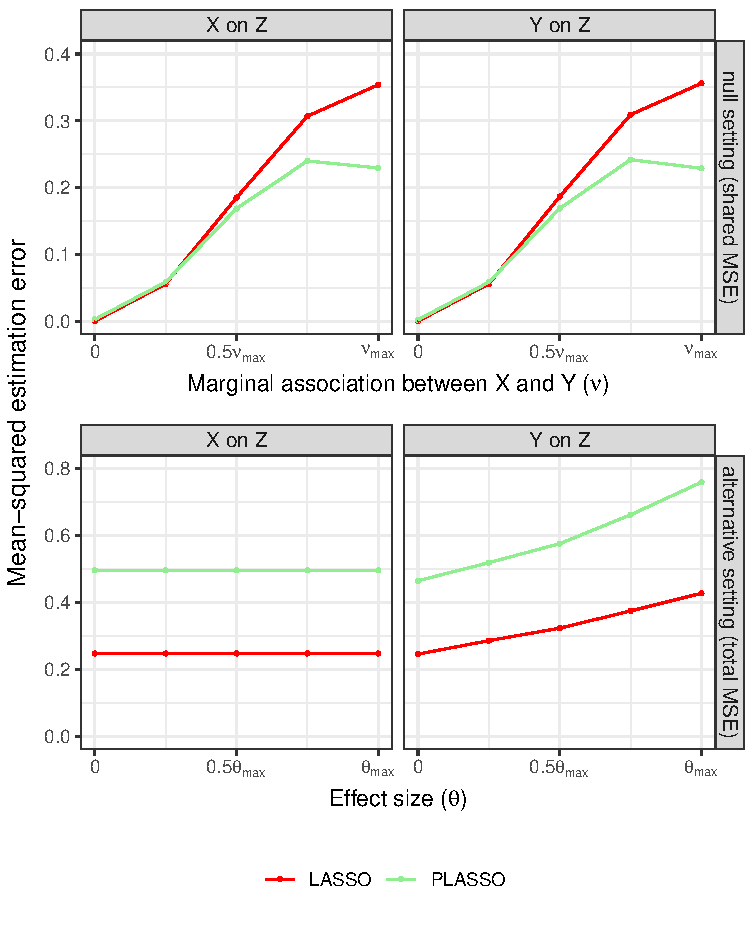
\includegraphics[width = 0.75\textwidth]{figures/MSE.pdf}
	\caption{MSE on shared variables and total variables: first column displays the MSE of lasso and post-lasso on shared active variables $Z_{\mathcal{A}}$ and the second column displays the MSE of lasso and post-lasso on total variables. All the experiments are carried out with GCM statistic with $n=100,d=400,s=5,\rho=0.4$. All the standard errors are less than 0.014.}
	\label{fig:MSE}
\end{figure}

\subsection{Additional simulation results} \label{sec:additional-simulation-results}

Figures \ref{fig:gaussian_supervised_null}-\ref{fig:binomial_semi-supervised_alternative} present the complete simulation results across the null and alternative, Gaussian and binary, and supervised and unsupervised settings. All the standard errors are less than 0.026.

\begin{figure}[!ht]
	\centering
	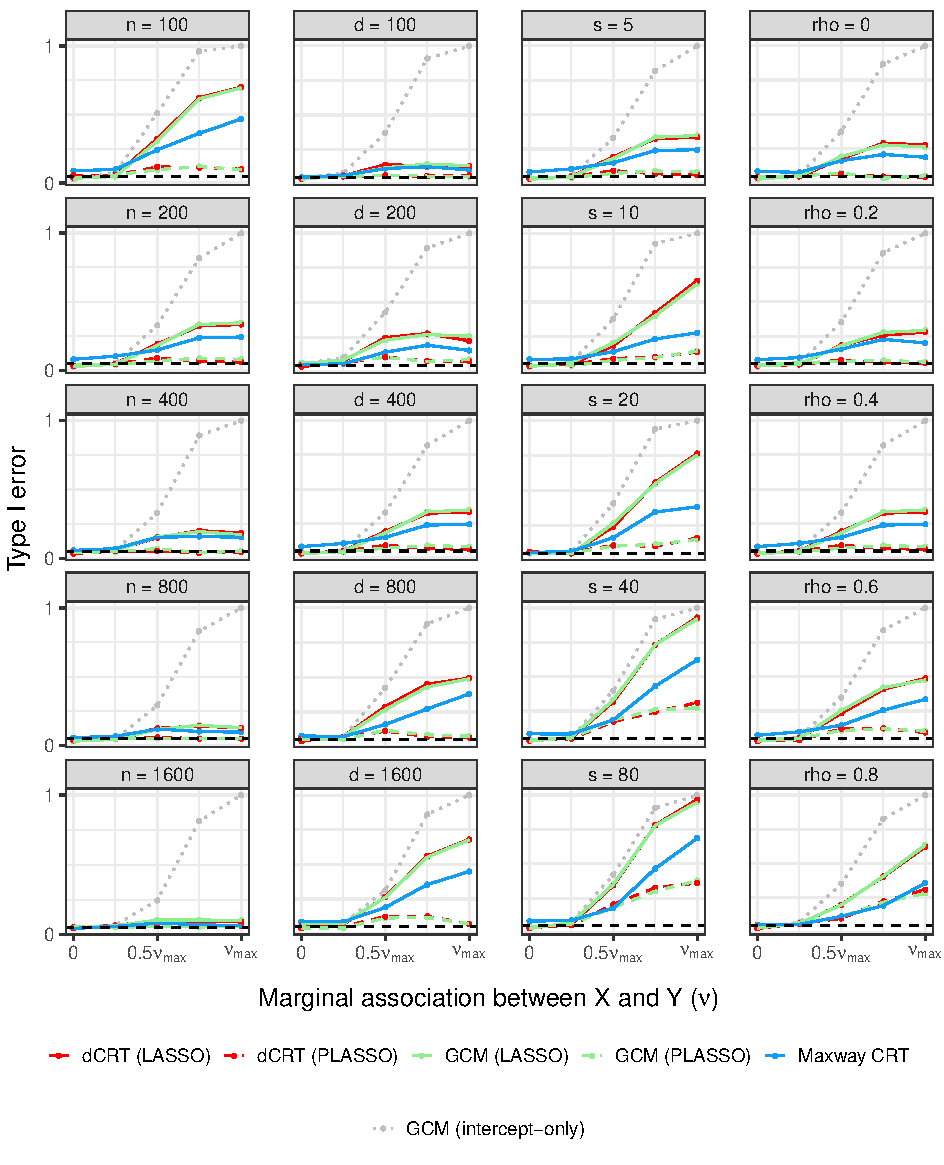
\includegraphics[width = \textwidth]{figures/gaussian_supervised_setting_null.pdf}
	\caption{Type-I error in the Gaussian supervised setting.}
	\label{fig:gaussian_supervised_null}
\end{figure}

\begin{figure}[!ht]
	\centering
	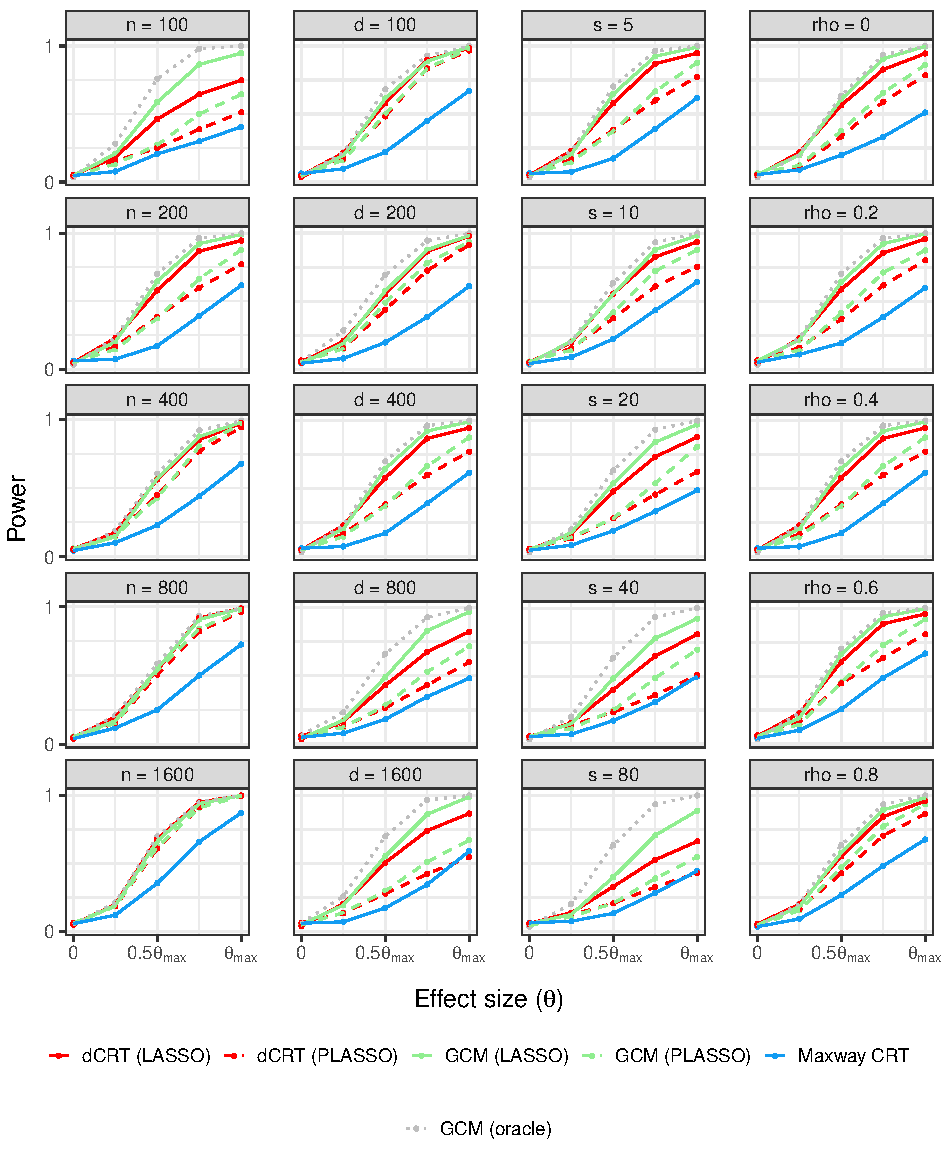
\includegraphics[width = \textwidth]{figures/gaussian_supervised_setting_alternative.pdf}
	\caption{Power in the Gaussian supervised setting.}
	\label{fig:gaussian_supervised_alternative}
\end{figure}

\begin{figure}[!ht]
	\centering
	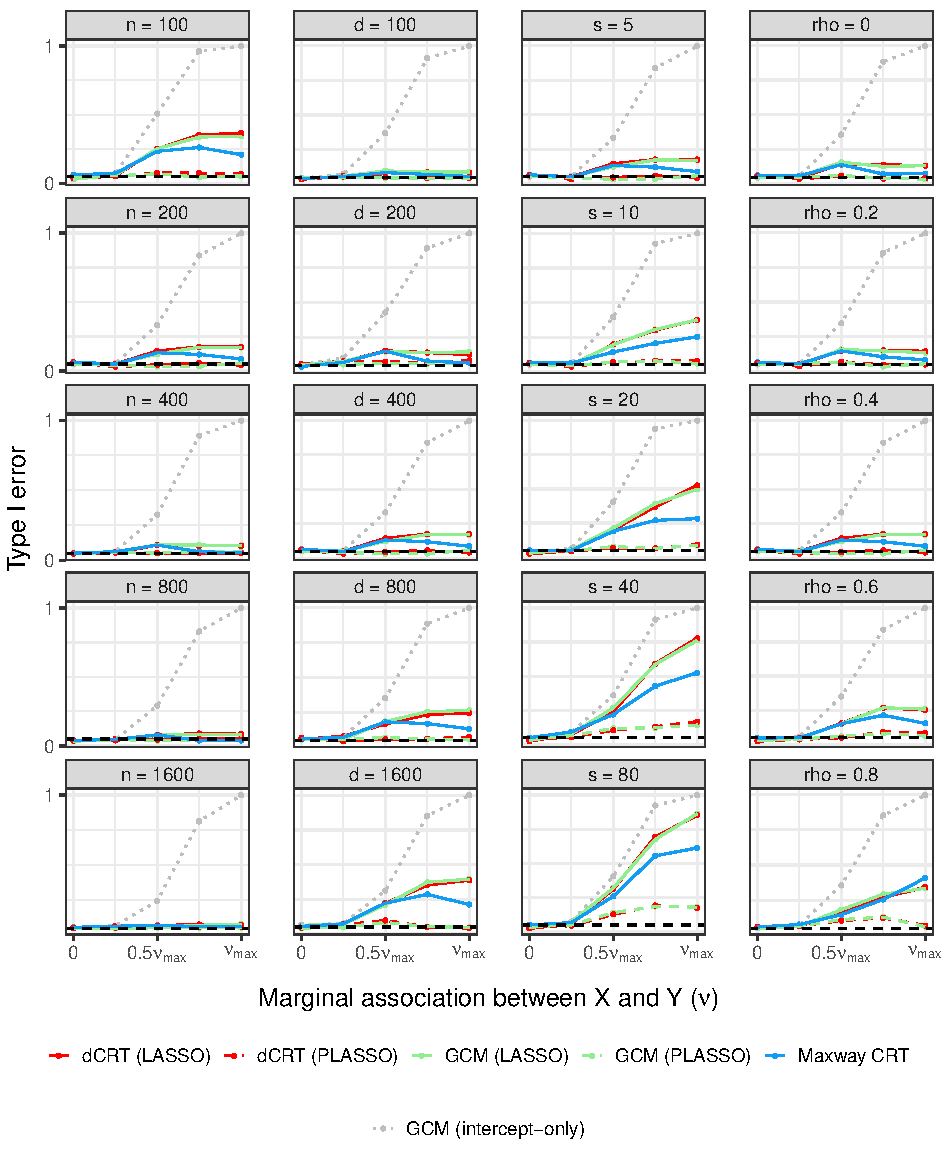
\includegraphics[width = \textwidth]{figures/gaussian_semi_supervised_setting_null.pdf}
	\caption{Type-I error in the Gaussian semi-supervised setting.}
	\label{fig:gaussian_semi-supervised_null}
\end{figure}


\begin{figure}[!ht]
	\centering
	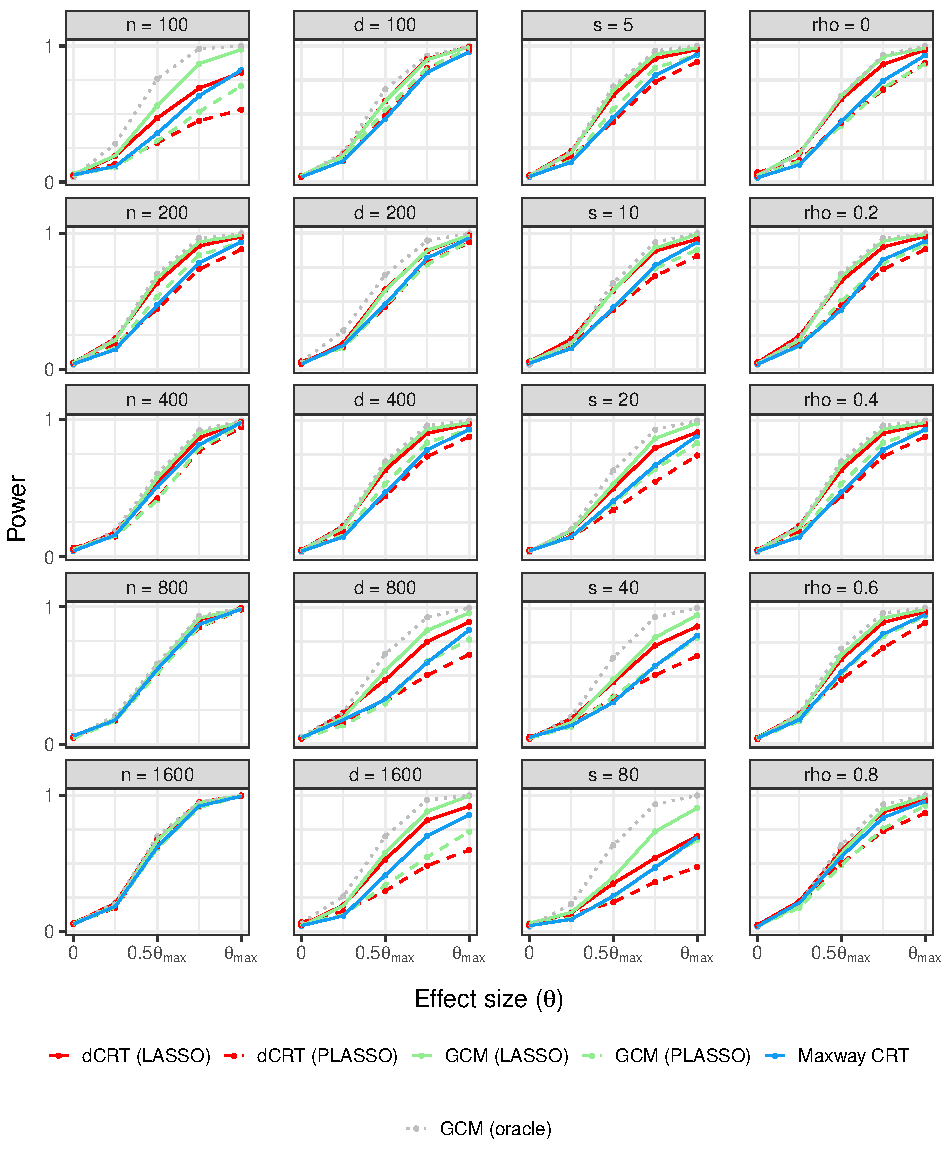
\includegraphics[width = \textwidth]{figures/gaussian_semi_supervised_setting_alternative.pdf}
	\caption{Power in the Gaussian semi-supervised setting.}
	\label{fig:gaussian_semi-supervised_alternative}
\end{figure}


\begin{figure}[!ht]
	\centering
	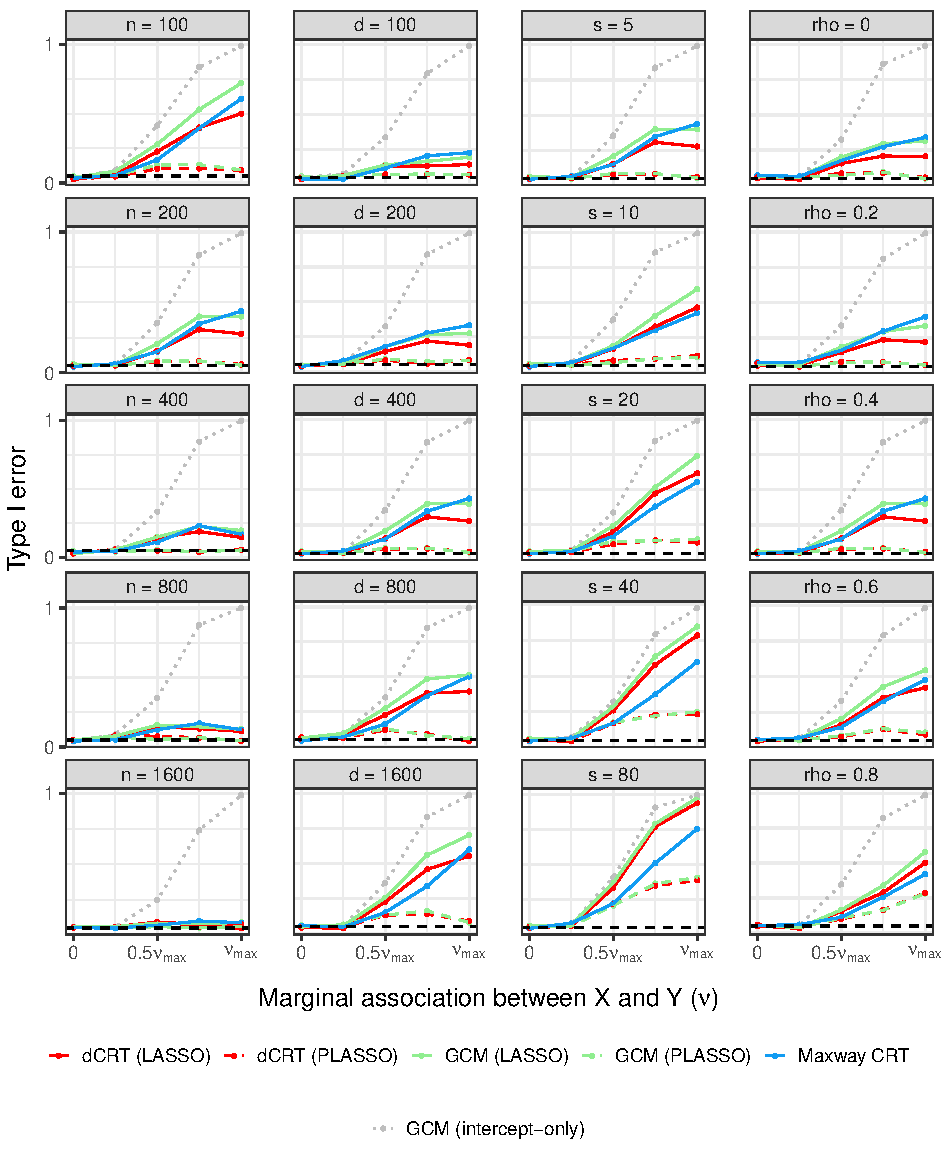
\includegraphics[width = \textwidth]{figures/binomial_supervised_setting_null.pdf}
	\caption{Type-I error in the binary supervised setting.}
	\label{fig:binomial_supervised_null}
\end{figure}

\begin{figure}[!ht]
	\centering
	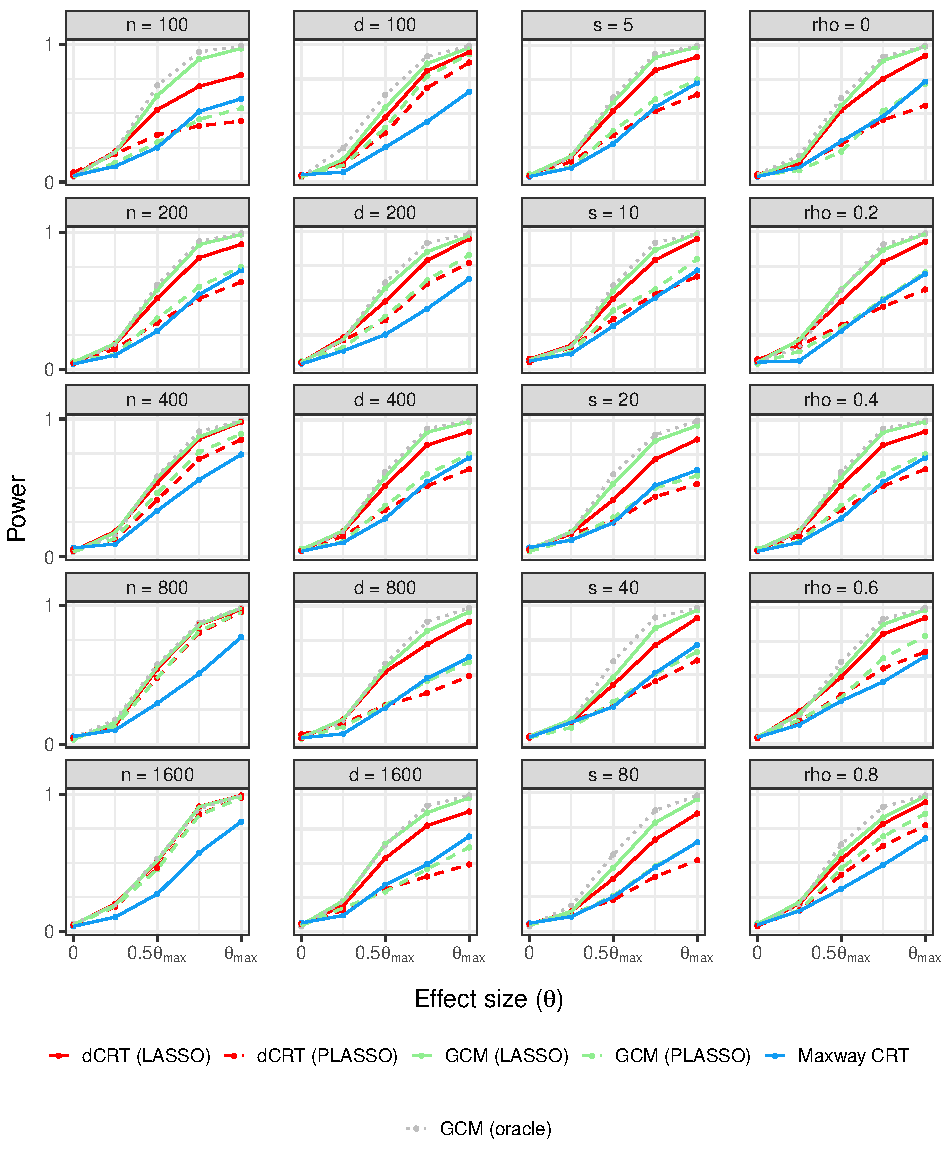
\includegraphics[width = \textwidth]{figures/binomial_supervised_setting_alternative.pdf}
	\caption{Power in the binary supervised setting.}
	\label{fig:binomial_supervised_alternative}
\end{figure}


\begin{figure}[!ht]
	\centering
	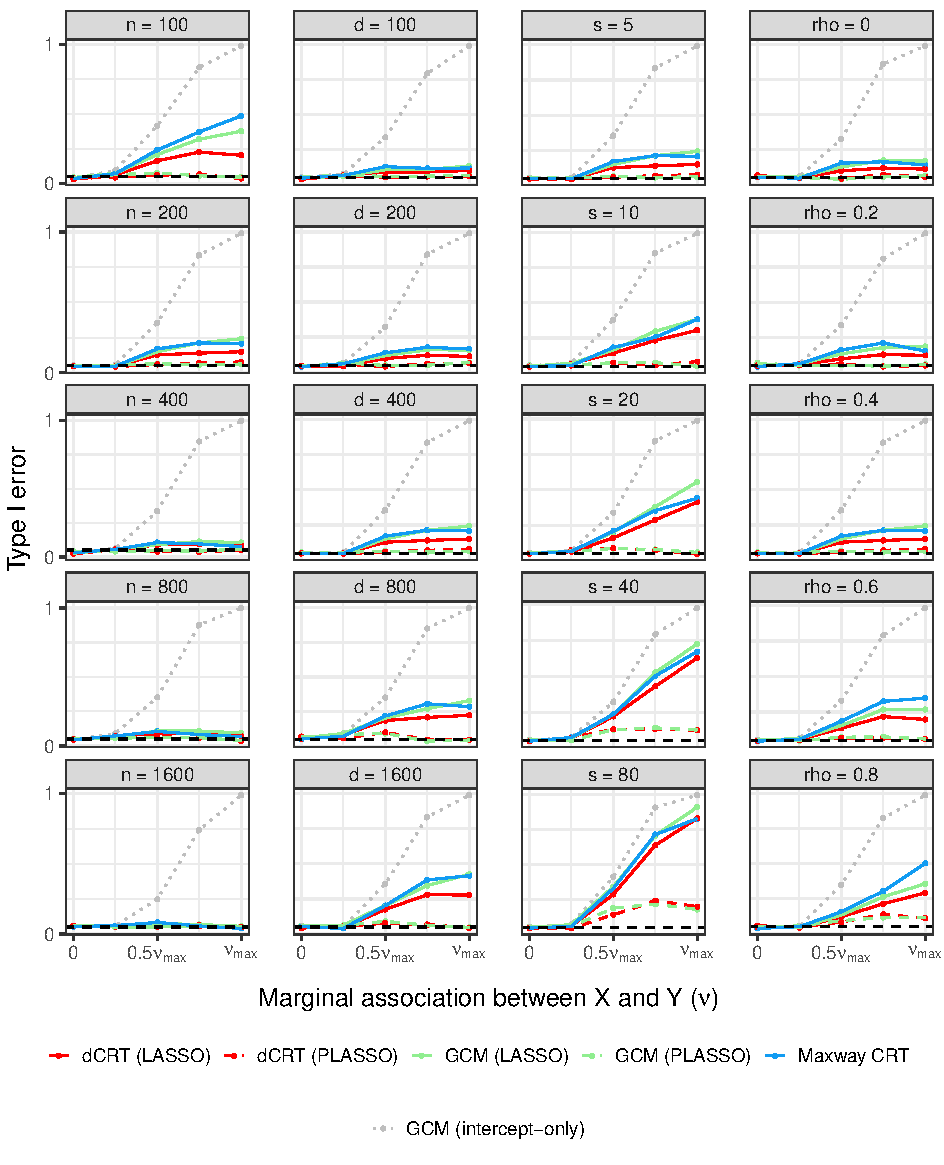
\includegraphics[width = \textwidth]{figures/binomial_semi_supervised_setting_null.pdf}
	\caption{Type-I error in the binary semi-supervised setting.}
	\label{fig:binomial_semi-supervised_null}
\end{figure}


\begin{figure}[!ht]
	\centering
	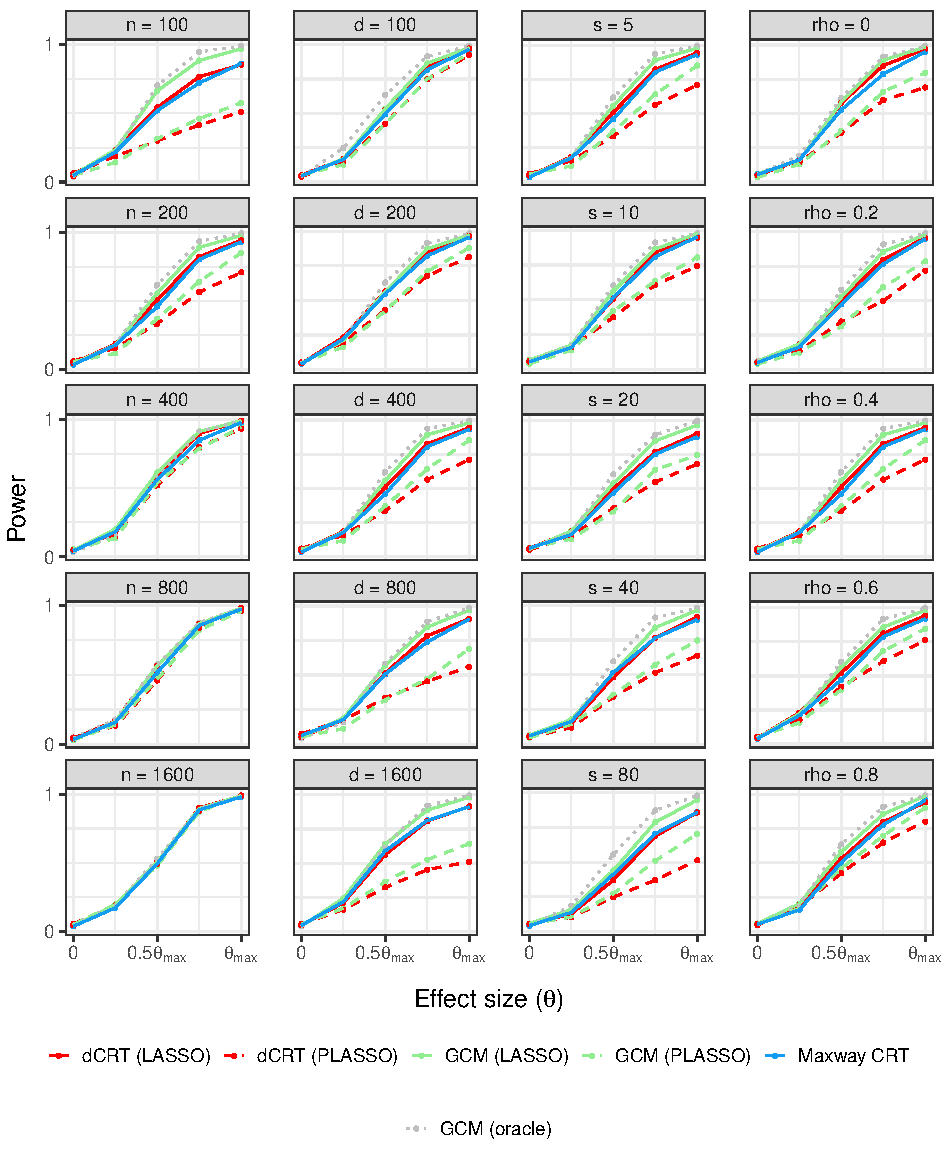
\includegraphics[width = \textwidth]{figures/binomial_semi_supervised_setting_alternative.pdf}
	\caption{Power in the binary semi-supervised setting.}
	\label{fig:binomial_semi-supervised_alternative}
\end{figure}

% \begin{figure}[!ht]
% 	\centering
% 	\includegraphics[scale = 1]{figures/gaussian_supervised_setting_dCRT.pdf}
% 	\caption{Gaussian supervised null setting with dCRT statistic}
% 	\label{fig:gaussian_supervised_dCRT}
% \end{figure}

% \begin{figure}[!ht]
% 	\centering
% 	\includegraphics[scale = 1]{figures/binomial_supervised_setting_dCRT.pdf}
% 	\caption{Binomial supervised null setting with dCRT statistic}
% 	\label{fig:binomial_supervised_dCRT}
% \end{figure}

\clearpage

\section{Proofs of conditional convergence results} \label{sec:conditional-convergence-proofs}

In this section, we present the proofs of the conditional convergence results from Appendix~\ref{sec:conditional-convergence-results}. We proceed by stating and proving necessary lemmas in Section~\ref{sec:conditional-convergence-lemmas} and then proving the convergence results themselves in Section~\ref{subsec:conditional-convergence-proofs}.

\subsection{Auxiliary lemmas} \label{sec:conditional-convergence-lemmas}

First we state a few known results for the reader's convenience.

\begin{lemma}[\cite{Durrett2010}, Theorem 2.3.2]\label{lem:sub_subseq}
A sequence of random variables $W_n$ converges to a limit $W$ in probability if and only if every subsequence of $W_n$ has a further subsequence that converges to $W$ almost surely.
\end{lemma}

% \begin{lemma}[Polya's theorem, \cite{VDV1998}, Lemma 2.11]\label{lem:polya}
% 	If $F_n$ is a sequence of cumulative distribution functions such that $F_n(t) \rightarrow F(t)$ for all $t \in \R$ and continuous $F$, then
% 	\begin{align*}
% 		\sup_{t \in \R}|F_n(t)-F(t)|\rightarrow 0.
% 	\end{align*}
% \end{lemma}


% \begin{lemma}[\cite{bulinski2017conditional}, Theorem 1]\label{lem:cond_cf_conver}
%  	Suppose $\{W_{in},i=1.\ldots,n\}_{n\in\mathbb{N}}$ be an array of random variables which are independent conditionally on $\mathcal{F}_n$ in each row and $\mathrm{Var}[W_{in}|\mathcal{F}_n]<\infty$ almost surely for $i=1,\ldots,n$ and for all $n\in\mathbb{N}$. Assume that $s_n^2\equiv\mathrm{Var}[S_n|\mathcal{F}_n]>0$ almost surely where $S_n=\sum_{i=1}^nW_{in}$ for all $n$ large enough. Then for every $t\in\mathbb{R}$
% 	\begin{align*}
% 		\E\left[\exp\left\{it\frac{S_n-\E[S_n|\mathcal{F}_n]}{s_n}\right\}|\mathcal{F}_n\right]\convp\exp\left\{-\frac{t^2}{2}\right\},\ n\rightarrow\infty
% 	\end{align*}
% 	if and only if for any $\epsilon>0$,
% 	\begin{align*}
% 		\frac{1}{s_n^2}\sum_{i=1}^n\E\left[(W_{in}-\E[W_{in}|\mathcal{F}_n])^2\bm 1\{|W_{in}-\E[W_{in}|\mathcal{F}_n]|\geq \epsilon s_n\}\right]\convp0.
% 	\end{align*}
% \end{lemma}

\begin{lemma}[Conditional Markov inequality, \cite{Davidson2003}, Theorem 10.17]\label{lem:cond_markov}
Let $W$ be a random variable and let $\mathcal F$ be a $\sigma$-algebra. If for some $q > 0$ we have $\E[|W|^q] < \infty$, then for any $\epsilon$ we have
	\begin{align*}
		\P(|W|\geq\epsilon|\mathcal{F})\leq \frac{\E[|W|^q|\mathcal{F}]}{\epsilon^q} \quad \text{almost surely}.
	\end{align*}
\end{lemma}

\begin{lemma}[Conditional H\"older inequality, \cite{Swanson2019}, Theorem 6.60]\label{lem:cond_holder}
	Let $W_1$ and $W_2$ be random variables and let $\mathcal F$ be a $\sigma$-algebra. If for some $q_1, q_2 \in (1,\infty)$ with $\frac{1}{q_1} + \frac{1}{q_2} = 1$ we have $\E[|W_1|^{q_1}], \E[|W_2|^{q_2}] < \infty$, then
	\begin{align*}
		\E[|W_1 W_2| \mid \mathcal F] \leq (\E[|W_1|^{q_1} \mid \mathcal F])^{1/q_1}(\E[|W_2|^{q_2} \mid \mathcal F])^{1/q_2} \quad \text{almost surely}.
	\end{align*}
\end{lemma}


\begin{lemma}[\cite{RL2005}, Lemma 11.2.1]\label{lem:conver_quantile}
	Suppose $W_n \convd W$. If for given $\alpha \in (0,1)$ the CDF of $W$ is continuous and strictly increasing at $\Q_{\alpha}[W]$, then
	\begin{align*}
		\Q_{\alpha}[W_n] \rightarrow \Q_{\alpha}[W].
	\end{align*}
\end{lemma}

Next we establish that, without of loss of generality, all random variables, $\sigma$-algebras, and conditional expectations in a triangular array may be viewed as being defined on a common probability space.
\begin{lemma}[Embedding into a single probability space]\label{lem:embedding}
	Consider a sequence of probability spaces $\{(\P_n,\Omega_n,\mathcal{G}_n),n \geq 1\}$. For each $n$, let $\{W_{i,n}\}_{i \geq 1}$ be a collection of integrable random variables defined on $(\P_n,\Omega_n,\mathcal{G}_n)$ and let $\mathcal F_n \subseteq \mathcal G_n$ be a $\sigma$-algebra. Then there exists a single probability space $(\widetilde{\P}, \widetilde{\Omega}, \widetilde{\mathcal G})$, random variables $\{\widetilde W_{i,n}\}_{i,n \geq 1}$ on $(\widetilde{\P}, \widetilde{\Omega}, \widetilde{\mathcal G})$, and $\sigma$-fields $\widetilde{\mathcal F}_n \subseteq \widetilde{\mathcal G}$ for $n \geq 1$, such that for each $n$, the joint distribution of $(\{W_{i,n}\}_{i \geq 1}, \{\E[W_{i,n}\mid\mathcal F_n]\}_{i \geq 1})$ on $(\P_n,\Omega_n,\mathcal{G}_n)$ coincides with that of $(\{\widetilde W_{i,n}\}_{i \geq 1}, \{\E[\widetilde W_{i,n}\mid \widetilde{\mathcal F}_n]\}_{i \geq 1})$ on $(\widetilde{\P}, \widetilde{\Omega}, \widetilde{\mathcal G})$.
\end{lemma}

\begin{proof}%[Proof of Lemma \ref{lem:embedding}]
	Define the Cartesian product $\widetilde \Omega \equiv \prod_{n=1}^{\infty}\Omega_n$, the $\sigma$-algebra $\widetilde {\mathcal G}$ generated by measurable cylinders $\prod_{n = 1}^\infty A_n$  for $A_n \in \mathcal G_n$ and $A_n = \mathcal G_n$ for all but finitely many $n$, and the infinite product measure $\widetilde{\P}$ on the measurable space $(\widetilde \Omega, \widetilde{\mathcal G})$ \citep{Saeki1996}. On this probability space, define $\sigma$-algebras 
	\begin{equation}
		\widetilde{\mathcal F}_n \equiv \{\mathcal G_1 \times \cdots \times \mathcal G_{n-1} \times A_n \times\mathcal G_{n+1} \times \cdots: A_n \in \mathcal F_n\}		
	\end{equation}
	and random variables
	\begin{equation}
	\widetilde W_{in}(\omega) \equiv W_{in}(\omega_n)
	\label{eq:random-variables-embedding}
	\end{equation}
	for each $i, n \geq 1$. Next we claim that for each $i, n \geq 1$, the random variable
	\begin{equation}
	\E_{\widetilde{\P}}[\widetilde W_{in}|\widetilde{\mathcal F}_n](\omega) \equiv \E_{\P_n}[W_{in}|\mathcal F_n](\omega_n) \quad \text{for each } \omega \in \widetilde \Omega
	\label{eq:sigma-fields-embedding}
	\end{equation}
	is in fact a version of the conditional expectation $\E_{\widetilde{\P}}[\widetilde W_{in}|\widetilde{\mathcal F}_n]$. Indeed, it suffices to check that for each $A \equiv \mathcal G_1 \times \cdots \times \mathcal G_{n-1} \times A_n \times\mathcal G_{n+1} \times \cdots \in \widetilde{\mathcal F}_n$ we have 
	\begin{equation}
		\begin{split}
	\int_{A} \E_{\widetilde{\P}}[\widetilde W_{in}|\widetilde{\mathcal F}_n](\omega)d\widetilde{\P}(\omega) &\equiv \int_{A} \E_{\P_n}[W_{in}|\mathcal F_n](\omega_n) \mathrm{d}\widetilde{\P}(\omega) \\
	&= \int_{\prod_{n' \neq n} \Omega_{n'}} \int_{A_n} \E_{\P_n}[W_{in}|\mathcal F_n](\omega_n) \mathrm{d}\widetilde{\P}_n(\omega_n)\mathrm{d}\prod_{n'\neq n}\P_{n'}(\omega_{n'}) \\
	&\equiv \int_{\prod_{n' \neq n} \Omega_{n'}} \int_{A_n} W_{in}(\omega_n) \mathrm{d}\widetilde{\P}_n(\omega_n)\mathrm{d}\prod_{n'\neq n}\P_{n'}(\omega_{n'}) \\
	&= \int_{A} W_{in}(\omega_n) \mathrm{d}\widetilde{\P}(\omega) \\
	&\equiv \int_{A} \widetilde W_{in}(\omega)d\widetilde{\P}(\omega).
		\end{split}
	\end{equation}
	From the $\omega$-wise embeddings~\eqref{eq:random-variables-embedding} and~\eqref{eq:sigma-fields-embedding}, it is easy to verify the claimed equality between the joint distributions on $(\P_n,\Omega_n,\mathcal{G}_n)$ and $(\widetilde{\P}, \widetilde{\Omega}, \widetilde{\mathcal G})$.
\end{proof}

Finally, we state a conditional version of the truncated weak law of large numbers:
\begin{lemma}\label{lem:cond_wlln}
	For each $n$, let $W_{in},1\leq i\leq n$ be a set of random variables independent conditionally on $\mathcal{F}_n$. Let $b_n>0$ with $b_n\rightarrow\infty$ and let $\Bar W_{in}=W_{in}\indicator(|W_{in}|\leq b_n)$. Suppose that as $n\rightarrow\infty$ we have
	\begin{enumerate}
		\item $\sum_{i=1}^{n}\P[|W_{in}|>b_n|\mathcal{F}_n]\convp0$ and
		\item $b_n^{-2}\sum_{i=1}^n\E[\Bar W_{in}^2|\mathcal{F}_n]\convp0$.
	\end{enumerate}
	If we set $S_n\equiv\sum_{i = 1}^n W_{in}$ and $a_n \equiv \sum_{i=1}^n\E[\Bar W_{in}]$ then
	\begin{align*}
		\frac{S_n - a_n}{b_n} \mid \mathcal{F}_n \convpp 0.
	\end{align*}
\end{lemma}
\begin{proof}
	Let $\Bar{S}_n \equiv \sum_{i = 1}^n \Bar W_{in}$. We first write
	\begin{align*}
		\P\left[\left|\frac{S_n-a_n}{b_n}\right|>\epsilon\bigg|\mathcal{F}_n\right]\leq \P\left[S_n\neq\Bar{S}_n|\mathcal{F}_n\right]+\P\left[\left|\frac{\Bar{S}_n-a_n}{b_n}\right|>\epsilon\bigg|\mathcal{F}_n\right].
	\end{align*}
	To estimate the first term, we note that
	\begin{align*}
		\P[S_n\neq\Bar{S}_n|\mathcal{F}_n]\leq \P[\cup_{i=1}^n\{\Bar W_{in}\neq W_{in}\}|\mathcal{F}_n] \leq \sum_{i=1}^n\P(|W_{in}|>b_n|\mathcal{F}_n)\convp0
	\end{align*}
	by the first assumption. For the second term, we note that conditional Markov's inequality (Lemma \ref{lem:cond_markov}), $a_n=\E[\Bar{S}_n|\mathcal{F}_n]$ implies that
	\begin{align*}
		\P\left[\left|\frac{\Bar{S}_n-a_n}{b_n}\right|>\epsilon|\mathcal{F}_n\right]
		&
		\leq \epsilon^{-2}\E\left[\left|\frac{\Bar{S}_n-a_n}{b_n}\right|^2\bigg|\mathcal{F}_n\right]\\
		&
		=\epsilon^{-2}b_n^{-2}\mathrm{Var}[\Bar{S}_n|\mathcal{F}_n]\\
		&
		=(b_n\epsilon)^{-2}\sum_{i=1}^n\mathrm{Var}[\Bar W_{in}|\mathcal{F}_n]\\
		&
		\leq (b_n\epsilon)^{-2}\sum_{i=1}^{n}\E\left[\Bar{X}^2_{in}|\mathcal{F}_n\right]\convp0,
	\end{align*}
	where the convergence in the last line is given by the second assumption. This completes the proof.
\end{proof}

% Next, we state a slightly stronger version of L\'{e}vy's continuity theorem \citep[Theorem 2.13]{VDV1998}:
% \begin{lemma} \label{lem:stronger-levy}
% 	Consider a sequence of random variables $W_n$ with characteristic functions $\phi_n(s)$ and a limiting random variable $W$ with characteristic function $\phi(s)$. There exists a countable set $S \subset \R$ such that, if $\phi_n(s) \rightarrow \phi(s)$ for each $s \in S$, then $W_n \convd W$.
% \end{lemma}
% \begin{proof}
% \textcolor{red}{TBD.}
% \end{proof}
% Next we claim that in-probability convergence of characteristic functions can be strengthened to uniform in-probability convergence of characteristic functions.
% \begin{lemma} \label{lem:pointwise-to-uniform-characteristic}
% If $\mathbb E[\exp(isW_n)|\mathcal F_n] \convp \mathbb E[\exp(isW)]$ for each $s \in \R$, then we also have
% \begin{equation}
%  \sup_{s \in \R} \left|\mathbb E[\exp(isW_n)|\mathcal F_n] - \mathbb E[\exp(isW)]\right| \convp 0.
% \end{equation}
% \end{lemma}
% \begin{proof}
% 	\textcolor{red}{TBD.}
% \end{proof}
	
	\subsection{Proofs of conditional convergence results} \label{subsec:conditional-convergence-proofs}
	
	\begin{proof}[Proof of Theorem~\ref{thm:cond_polya}] 
		This proof generalizes the argument of \cite[Lemma 2.11]{VDV1998} to allow for conditioning. Fix $\epsilon > 0$, and choose an integer $k \geq 2/\epsilon$. Because the CDF of $W$ is continuous, it follows that 
		\begin{equation*}
			\P[W \leq \Q_{i/k}[W]] = i/k \quad \text{for each }0 \leq i \leq k.
		\end{equation*}
		Fix $t \in \R$, and suppose $\Q_{\frac{i-1}{k}}[W] \leq t \leq \Q_{\frac i k}[W]$. It follows that 
		\begin{equation*}
			\P[W_n \leq \Q_{\frac{i-1}{k}}[W] \mid \mathcal F_n] - \frac{i}{k} \leq \P[W_n \leq t \mid \mathcal F_n] - \P[W \leq t] \leq \P[W_n \leq \Q_{\frac i k}[W] \mid \mathcal F_n] - \frac{i-1}{k}.
		\end{equation*}
		Therefore, for all $t \in \R$, we have
		\begin{equation*}
			\begin{split}
				|\P[W_n \leq t \mid \mathcal F_n] - \P[W \leq t]| &\leq \sup_{0 \leq i \leq k} \left|\P[W_n \leq \Q_{i/k}[W] \mid \mathcal F_n] - \frac{i}{k}\right| + \frac 1 k \\
				&=  \sup_{0 \leq i \leq k} \left|\P[W_n \leq \Q_{\frac i k}[W] \mid \mathcal F_n] - \mathbb P[W \leq \Q_{\frac i k}[W]]\right| + \frac{1}{k},
			\end{split}
		\end{equation*}
		so that
		\begin{equation*}
			\sup_{t \in \R}|\P[W_n \leq t \mid \mathcal F_n] - \P[W \leq t]| \leq \sup_{0 \leq i \leq k} \left|\P[W_n \leq \Q_{\frac i k}[W] \mid \mathcal F_n] - \mathbb P[W \leq \Q_{\frac i k}[W]]\right| + \frac{1}{k}.
		\end{equation*}
		By assumption, we have
		\begin{equation}
			\P\left[\left|\P[W_n \leq \Q_{\frac i k}[W] \mid \mathcal F_n] - \mathbb P[W \leq \Q_{\frac i k}[W]]\right| > \frac{1}{k(k+1)}\right] \rightarrow 0. 
		\end{equation}
		Therefore, 
		\begin{equation*}
			\begin{split}
				&\P\left[\sup_{t \in \R}|\P[W_n \leq t \mid \mathcal F_n] - \P[W \leq t]| > \epsilon \right] \\
				&\quad\leq \P\left[\sup_{t \in \R}|\P[W_n \leq t \mid \mathcal F_n] - \P[W \leq t]| > \frac{2}{k} \right] \\
				&\quad\leq \P\left[\sup_{0 \leq i \leq k} \left|\P[W_n \leq \Q_{\frac i k}[W] \mid \mathcal F_n] - \mathbb P[W \leq \Q_{\frac i k}[W]]\right| > \frac{1}{k} \right] \\
				&\quad\leq \sum_{i = 0}^k  \P\left[ \left|\P[W_n \leq \Q_{\frac i k}[W] \mid \mathcal F_n] - \mathbb P[W \leq \Q_{\frac i k}[W]]\right| > \frac{1}{k(k+1)} \right] \\
				&\quad \rightarrow 0.
			\end{split}
		\end{equation*}
		This completes the proof.
	\end{proof}
	
	\begin{proof}[Proof of Theorem \ref{thm:cond_slutsky}]
		Fix $t \in \R$. Letting $F(t') \equiv \P[W \leq t']$ be the CDF of $W$, Theorem \ref{thm:cond_polya} gives 
		\begin{align*}
			\left|\P\left[W_n\leq \frac{t - b_n}{a_n}\mid\mathcal{F}_n\right]-F\left(\frac{t - b_n}{a_n}\right)\right| \leq	\sup_{t' \in \R}|\P[W_n\leq t'|\mathcal{F}_n]-F(t')|\convp0.
		\end{align*}
		By the continuous mapping theorem, we have $F\left(\frac{t - b_n}{a_n}\right) \convp F(t)$, so that
		\begin{equation*}
			\P\left[W_n\leq \frac{t - b_n}{a_n}\mid\mathcal{F}_n\right] \convp F(t).
		\end{equation*}
		Noting that $\P[a_n \leq 0 | \mathcal F_n]$ is a sequence of nonnegative random variables whose expectations converge to zero, it follows that $\P[a_n \leq 0 | \mathcal F_n] \convp 0$ and so
		\begin{equation*}
			\begin{split}
				\P\left[a_nW_n + b_n \leq t \mid\mathcal{F}_n\right] &= \P\left[a_nW_n + b_n \leq t, a_n > 0\mid\mathcal{F}_n\right] + o_p(1) \\
				&= \P\left[W_n\leq \frac{t - b_n}{a_n}, a_n > 0\mid\mathcal{F}_n\right] + o_p(1) \\
				&= \P\left[W_n\leq \frac{t - b_n}{a_n}\mid\mathcal{F}_n\right] + o_p(1) \\
				&\convp F(t),
			\end{split}
		\end{equation*}
		as desired.
	\end{proof}
	
	
	\begin{proof}[Proof of Theorem \ref{thm:wlln_cond}] 
		We apply Lemma \ref{lem:cond_wlln} with $b_n=n$. We first verify the first assumption in Lemma \ref{lem:cond_wlln} by conditional Markov's inequality (Lemma \ref{lem:cond_markov}):
		\begin{align*}
			\sum_{i=1}^n\P(|W_{in}|>n|\mathcal{F}_n)\leq \sum_{i=1}^n\frac{\E(|W_{in}|^{1+\delta}|\mathcal{F}_n)}{n^{1+\delta}}\convp0.
		\end{align*}
		For the second condition, we have
		\begin{align*}
			\frac{1}{n^{2}}\sum_{i=1}^n\E[W_{in}^2\indicator(|W_{in}|\leq n)|\mathcal{F}_n]
			&
			\leq \frac{1}{n^2}\sum_{i=1}^n\E[|W_{in}|^{1+\delta}n^{1-\delta}\indicator(|W_{in}|\leq n)]\\
			&
			= \frac{1}{n^{1+\delta}}\sum_{i=1}^n\E[|W_{in}|^{1+\delta}\indicator(|W_{in}|\leq n)|\mathcal{F}_n]\\
			&
			\leq \frac{1}{n^{1+\delta}}\sum_{i=1}^n\E[|W_{in}|^{1+\delta}|\mathcal{F}_n]\convp0.
		\end{align*}
		Therefore, Lemma~\ref{lem:cond_wlln} yields
		\begin{align*}
			\left.\frac1n\sum_{i=1}^n (W_{in}-\E[W_{in}\indicator(|W_{in}|\leq n) \mid \mathcal{F}_n]) \ \right|\ \mathcal{F}_n \convpp 0.
		\end{align*}
		By conditional Slutsky (Theorem~\ref{thm:cond_slutsky}), it now suffices to show that
		\begin{align*}
			\frac{1}{n}\sum_{i=1}^n\E\left[W_{in}\indicator(|W_{in}| > n) \mid \mathcal{F}_n\right] \convp 0.
		\end{align*}
		To see this, applying conditional Markov's and H\"older's inequalities (Lemmas~\ref{lem:cond_markov} and~\ref{lem:cond_holder}, respectively) we obtain
		\begin{align*}
			\left|\frac{1}{n}\sum_{i=1}^n\E\left[W_{in}\indicator(|W_{in}| > n)|\mathcal{F}_n\right]\right|
			&
			\leq \frac{1}{n}\sum_{i=1}^n\E\left[|W_{in}|\indicator(|W_{in}| > n)|\mathcal{F}_n\right]\\
			&
			\leq\frac{1}{n}\sum_{i=1}^n\{\E[|W_{in}|^{1+\delta}|\mathcal{F}_n]\}^{1/(1+\delta)}\{\P[|W_{in}|>n|\mathcal{F}_n]\}^{\delta/(1+\delta)} \\
			&
			\leq \frac{1}{n}\sum_{i=1}^n\{\E[|W_{in}|^{1+\delta}|\mathcal{F}_n]\}^{1/(1+\delta)}\left\{\frac{\E(|W_{in}|^{1+\delta}|\mathcal{F}_n)}{n^{1+\delta}}\right\}^{\delta/(1+\delta)}\\
			&
			=\frac{1}{{n^{1+\delta}}}\sum_{i=1}^n\E[|W_{in}|^{1+\delta}|\mathcal{F}_n]\\
			&
			\convp0,
		\end{align*}
		where the last convergence is by assumption. Finally, we verify that the condition~\eqref{eq:wlln_cond_sufficient} is sufficient for the conditional WLLN assumption~\eqref{eq:wlln_cond_assumption} by noting that it implies
		\begin{align*}
			\frac{1}{n^{1+\delta}} \sum_{i = 1}^n \E[|W_{in}|^{1+\delta} \mid \mathcal{F}_n]\leq \frac{\sup_{1\leq i\leq n}\E[|W_{in}|^{1+\delta} \mid \mathcal{F}_n]n}{n^{1+\delta}}=\frac{\sup_{1\leq i\leq n}\E[|W_{in}|^{1+\delta} \mid \mathcal{F}_n]}{n^{\delta}} \convp 0.
		\end{align*}
		This completes the proof.
	\end{proof}
	
	\begin{proof}[Proof of Theorem \ref{thm:conditional-clt}] 
		Without loss of generality, we assume $\E[W_{in}|\mathcal{F}_n]=0$ and that all random variables and $\sigma$-algebras are defined on a common probability space $(\P, \Omega, \mathcal G)$ (Lemma~\ref{lem:embedding}). Let $\mathcal B(\R^n)$ be the Borel $\sigma$-algebra on $\R^n$. Let $\kappa_{n}$ be a regular conditional distribution of $(W_{1n}, \dots, W_{nn})$ given $\mathcal{F}_{n}$ \citep[Theorem 8.37]{Lista2017}, i.e. a function $\kappa_{n}: \Omega \times \mathcal B(\R^n) \rightarrow [0,\infty]$ such that $\omega \mapsto \kappa_{n}(\omega, B)$ is measurable for each $B \in \mathcal B(\R^n)$, $B \mapsto \kappa_{n}(\omega, B)$ is a $\sigma$-finite measure on $\R^n$ for each $\omega \in \Omega$, and 
		\begin{align*}
			\kappa_{n}(\omega, B) = \P[(W_{1n}, \dots, W_{nn})\in B|\mathcal{F}_{n}](\omega), \quad \text{for almost all } \omega \in \Omega \text{ and all} \ B \in \mathcal B(\R^n).
			%		\label{eq:rcd}
		\end{align*}
		For each $n$ and each $\omega \in \Omega$, let $(\widetilde W_{1n}(\omega), \dots, \widetilde W_{nn}(\omega))$ be a draw from the measure $\kappa_n(\omega,\cdot)$. By \citet[Theorem 8.38]{Lista2017}, we have for each $n$ that
		\begin{equation*}
			\left(\sum_{i = 1}^n \V[\widetilde W_{in}(\omega)]\right)^{-(2+\delta)/2}\sum_{i = 1}^n \E[|\widetilde W_{in}(\omega)|^{2+\delta}] \overset{a.s.}= \frac{1}{S_{n}^{2+\delta}(\omega)} \sum_{i = 1}^{n} \E[|W_{in}|^{2+\delta} \mid \mathcal{F}_{n}](\omega).
		\end{equation*}
		Now, let $\{n_k\}_{k \geq 1}$ be a subsequence of $\mathbb N$. By the conditional Lyapunov assumption~\eqref{eq:conditional-lyapunov} and Lemma~\ref{lem:sub_subseq}, there is a further subsequence $n_{k_j}$ such that
		\begin{equation}
			\frac{1}{S_{n_{k_j}}^{2+\delta}} \sum_{i = 1}^{n_{k_j}} \E[|W_{in_{k_j}}|^{2+\delta} \mid \mathcal{F}_{n_{k_j}}] \convas 0.
		\end{equation}
		Hence, it follows that 
		\begin{equation}
			\left(\sum_{i = 1}^{n_{k_j}} \V[\widetilde W_{in_{k_j}}(\omega)]\right)^{-(2+\delta)/2}\sum_{i = 1}^{n_{k_j}} \E[|\widetilde W_{i{n_{k_j}}}(\omega)|^{2+\delta}] \rightarrow 0 \quad \text{for almost every } \omega \in \Omega.
		\end{equation}
		Applying the usual Lyapunov CLT to the triangular array $\{\widetilde W_{in_{k_j}}(\omega)\}_{i,n_{k_j}}$, we find that
		\begin{equation}
			\left(\sum_{i = 1}^{n_{k_j}} \V[\widetilde W_{in_{k_j}}(\omega)]\right)^{-1/2}\sum_{i = 1}^{n_{k_j}} \widetilde W_{in_{k_j}}(\omega) \convd N(0,1) \quad \text{for almost every } \omega \in \Omega,
		\end{equation}
		and therefore that, for each $t \in \R$, we have 
		\begin{equation}
			\mathbb P\left[\left(\sum_{i = 1}^{n_{k_j}} \V[\widetilde W_{in_{k_j}}(\omega)]\right)^{-1/2}\sum_{i = 1}^{n_{k_j}} \widetilde W_{in_{k_j}}(\omega) \leq t\right] \rightarrow \Phi(t) \quad \text{for almost every } \omega \in \Omega.
		\end{equation}
		Using \citet[Theorem 8.38]{Lista2017} again, it follows that for each $t \in \R$, we have
		\begin{equation}
			\mathbb P\left[\frac{1}{S_{n_{k_j}}}\sum_{i = 1}^{n_{k_j}} W_{in_{k_j}} \leq t \mid \mathcal F_{n_{k_j}}\right] \convas \Phi(t).
		\end{equation}
		Applying Lemma~\ref{lem:sub_subseq}, it follows that
		\begin{equation}
			\mathbb P\left[\frac{1}{S_{n}}\sum_{i = 1}^{n} W_{in} \leq t \mid \mathcal F_{n}\right] \convp \Phi(t),
		\end{equation}
		as desired.
	\end{proof}
	
	\begin{proof}[Proof of Lemma \ref{lem:conditional-convergence-to-quantile}]
		
		Without loss of generality, we assume that all random variables and $\sigma$-algebras are defined on a common probability space $(\P, \Omega, \mathcal G)$ (Lemma~\ref{lem:embedding}). Let $\mathcal B(\R)$ be the Borel $\sigma$-algebra on $\R$. Let $\kappa_{n}$ be a regular conditional distribution of $W_n$ given $\mathcal{F}_{n}$ \citep[Theorem 8.29]{Lista2017}, i.e. a function $\kappa_{n}: \Omega \times \mathcal B(\R) \rightarrow [0,\infty]$ such that $\omega \mapsto \kappa_{n}(\omega, B)$ is measurable for each $B \in \mathcal B(\R)$, $B \mapsto \kappa_{n}(\omega, B)$ is a $\sigma$-finite measure on $\R^n$ for each $\omega \in \Omega$, and 
		\begin{align*}
			\kappa_{n}(\omega, B) = \P[W_{n} \in B|\mathcal{F}_{n}](\omega), \quad \text{for almost all } \omega \in \Omega \text{ and all} \ B \in \mathcal B(\R).
		\end{align*}
		Now, let $\{n_k\}_{k \geq 1}$ be a subsequence of $\mathbb N$. By conditional Polya's theorem (Theorem~\ref{thm:cond_polya}), we have 
		\begin{equation}
			\sup_{t \in \R}|\P[W_{n}\leq t|\mathcal{F}_n]-\P[W\leq t]| \convp0.
		\end{equation}
		Hence, by Lemma~\ref{lem:sub_subseq} there is a further subsequence $n_{k_j}$ such that
		\begin{equation}
			\sup_{t \in \R}|\P[W_{n_{k_j}}\leq t|\mathcal{F}_{n_{k_j}}](\omega)-\P(W\leq t)|\rightarrow0,\ \text{for almost all } \omega \in \Omega.
		\end{equation}	
		It follows that 
		\begin{equation}
			\sup_{t \in \R}|\kappa_{n_{k_j}}(\omega, (-\infty, t])-\P(W\leq t)|\rightarrow0,\ \text{for almost all } \omega \in \Omega,
		\end{equation}
		i.e.
		\begin{equation}
			\kappa_{n_{k_j}}(\omega, \cdot) \convd W \ \text{for almost all } \omega \in \Omega.
		\end{equation}
		Hence, by Lemma~\ref{lem:conver_quantile}, it follows that
		\begin{equation}
			\Q_{\alpha}[\kappa_{n_{k_j}}(\omega, \cdot)] \rightarrow \Q_{\alpha}[W] \ \text{for almost all } \omega \in \Omega,
		\end{equation}
		and therefore
		\begin{equation}
			\Q_{\alpha}[W_{n_{k_j}}|\mathcal{F}_{n_{k_j}}] \convas \Q_{\alpha}[W].
		\end{equation}
		Applying Lemma~\ref{lem:sub_subseq} again, we conclude that
		\begin{equation}
			\Q_{\alpha}[W_{n}|\mathcal{F}_{n}] \convp \Q_{\alpha}[W],
		\end{equation}
		as desired.
	\end{proof}

	\section{Finite-sample improvement using $\ndCRThat$ over $\GCM$} \label{sec:finite-sample-improvement}

	We proved that the $\dCRThat$ and GCM test are asymptotically equivalent, both under the null and under local alternatives (Theorem \ref{thm:equivalence} and Corollary \ref{cor:asymptotic-equivalence-alternative}). Despite this asymptotic equivalence, the two methods can behave quite differently in finite samples. In particular, the resampling-based $\dCRThat$ method can have better finite-sample performance than the asymptotic $\GCM$ test. In this appendix, we present a simple numerical example to illustrate this phenomenon, focusing on the Type-I error of the two methods. In order to isolate the effect of the resampling rather than of the test statistic, we perform the comparison using the GCM test statistic for both methods. Therefore, we consider the $\ndCRThat$ variant (Appendix~\ref{sec:ndcrt}) rather than the $\dCRThat$ itself.

 	Consider the null data-generating model 
	\begin{align*}
		\bm Y\sim \textnormal{Poisson}(\mu_y(\bm Z)),\ \bm X\sim \textnormal{Bern}(\mu_x(\bm Z))
	\end{align*}
	where $\mu_y(\bm Z)=\exp(\beta_0+\bm Z\beta_1)$ and $\mu_x(\bm Z)=\textnormal{expit}(\gamma_0+\bm Z\gamma_1)$ and $\bm Z\sim N(0,1)$. In other words,
	$\bm Y|\bm Z$ is a Poisson regression model and $\bm X|\bm Z$ is a logistic regression model. We consider the following set of parameters:
	\begin{align*}
		\gamma_0=-4,\ \gamma_1=1,\ \beta_0= -3,\ \beta_1= 1,
	\end{align*}
	chosen to make both $\srx$ and $\sry$ sparse. Such a setting occurs commonly in single-cell genomics, and is one where we would expect the convergence of the central limit theorem to be slower. In this simulation, we take the sample size $n=1000$ and employ the usual generalized linear model estimates for $\mu_{x}(\cdot)$ and $\mu_y(\cdot)$. We set $M=1000$ when applying $\ndCRThat$ and the simulation is repeated $1000$ times. 
	\begin{figure*}
		\begin{subfigure}[b]{0.49\textwidth}
			\centering
			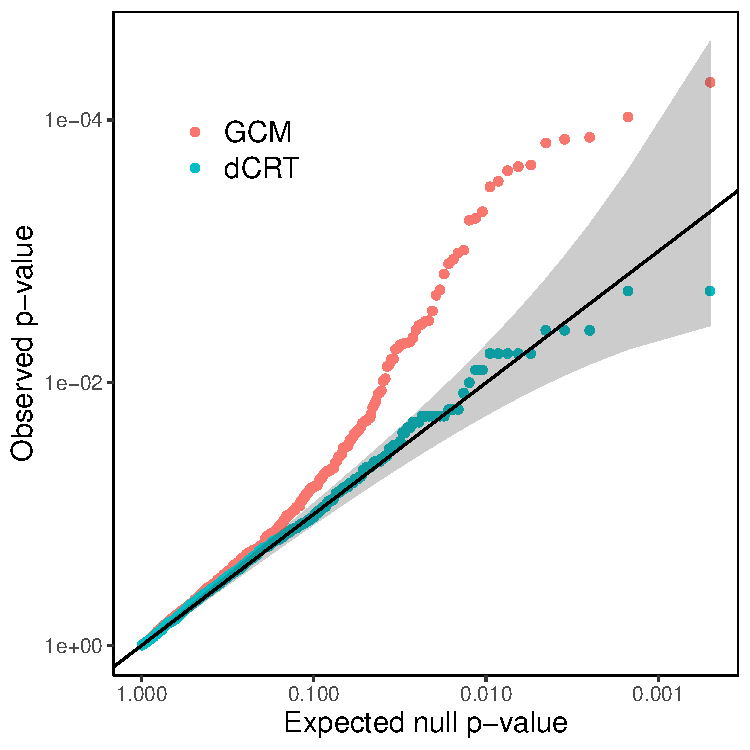
\includegraphics[width=\linewidth]{Figures/qq-plots.pdf} \\
		\end{subfigure}%
		\begin{subfigure}[b]{0.49\textwidth}
			\centering
			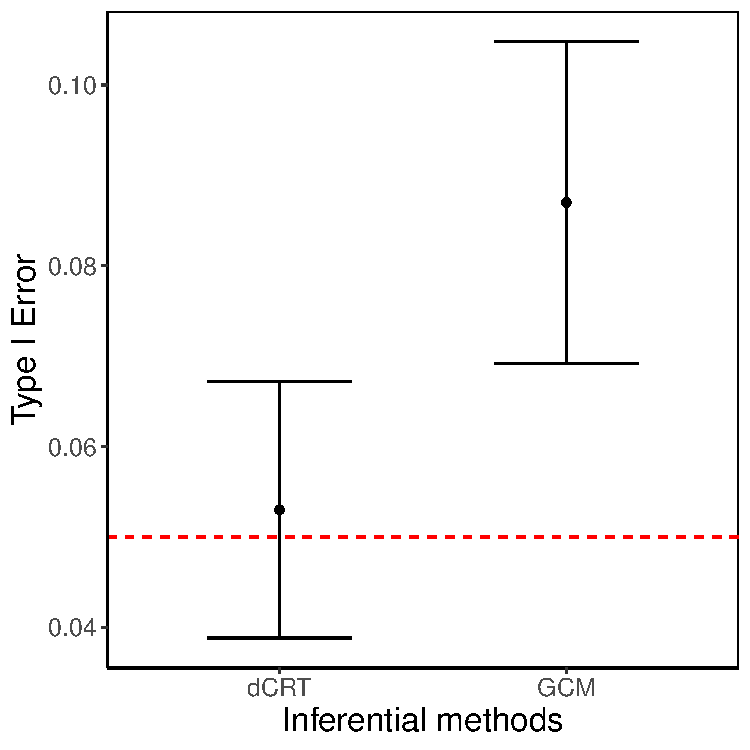
\includegraphics[width=\linewidth]{Figures/type_I_err_5e-2.pdf} \\ 
		\end{subfigure}
	
		\begin{subfigure}[b]{0.49\textwidth}
			\centering
			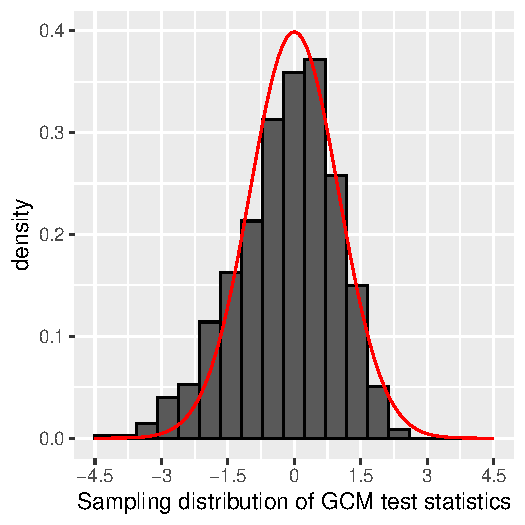
\includegraphics[width=\linewidth]{Figures/sampled-test-stats.pdf} \\ 
		\end{subfigure}%
		\begin{subfigure}[b]{0.49\textwidth}
			\centering
			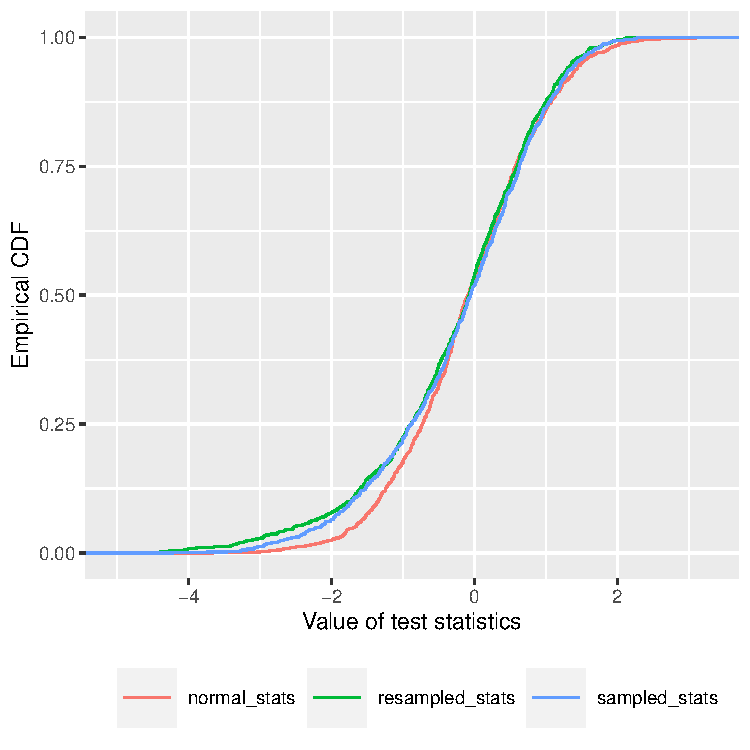
\includegraphics[width=\linewidth]{Figures/ecdf_comparison.pdf}
		\end{subfigure}
		\caption{Comparing the calibration of the $\GCM$ and $\ndCRThat$ methods in a sparse regime. Top left: QQ-plots of the $p$-values produced by the two methods in a null simulation setting. Top right: Type-I error of the two methods at $\alpha = 0.05$. Bottom left: The true null distribution of the GCM statistic (gray histogram), as well as the standard normal density (red curve). Bottom right: Comparisons of the empirical CDFs of the GCM test statistics, the $\ndCRThat$ resamples, and the standard normal distribution.}
		\label{fig:dCRT_GCM_binomial_poisson} 
	\end{figure*}

    Figure \ref{fig:dCRT_GCM_binomial_poisson} shows the results of the simulation. The top-left panel compares the $p$-values from the two methods across 1000 realizations of the data, showing that the $\ndCRThat$ produces well-calibrated $p$-values while the GCM test produces inflated $p$-values. Thresholding these $p$-values as nominal level $\alpha = 0.05$, we find that the $\ndCRThat$ method controls the Type-I error at the nominal level, while the GCM test does not (top-right panel). The reason for the miscalibration of the GCM test in this setting is that the null distribution of the test statistic has not yet converged to normality (bottom-left panel). By contrast, the resampling distribution of the GCM statistic (employed by the $\ndCRThat$ to obtain the critical value) aligns well with its null distribution (bottom-right panel), explaining the improved calibration of the $\ndCRThat$ method. Finally, the bottom-right panel shows the empirical CDF of the test statistics, which illustrates the difference in the null distributions of the two methods.

	\clearpage
	\section{Impact of the asymmetry of $\dCRThat$}

	As pointed out by a referee, the $\dCRThat$ is asymmetric in $\srx$ and $\sry$ while the conditional independence null hypothesis is symmetric in $\prx$ and $\pry$. One may obtain two different variants of the $\dCRThat$ by swapping the roles of $\srx$ and $\sry$. In this section, we investigate the impact of this asymmetry on the performance of the $\dCRThat$ test. 
	
	Intuition suggests that the $\dCRThat$ will have better performance if resampling is done based on the conditional distribution $\law_n(\prx \mid \prz)$ or $\law_n(\pry \mid \prz)$ that is estimated more accurately. To verify this intuition, we consider a simulation setting where the error in estimating $\law_n(\prx \mid \prz)$ is less than that in estimating $\law_n(\pry \mid \prz)$. In particular, we a null setting where $\law_n(\prx \mid \prz)$ and $\law_n(\pry \mid \prz)$ are Poisson regression models, where the coefficients in $\law_n(\prx \mid \prz)$ are smaller than those in $\law_n(\pry \mid \prz)$:
	\begin{align*}
		\bm X|\bm Z\sim \textnormal{Poisson}(\exp(-1+\bm Z^\top \beta)),\ \bm Y|\bm Z\sim \textnormal{Poisson}(\exp(-1+\bm Z^\top\gamma)),\ \bm Z\sim N(\bm 0,\bm I_p),
	\end{align*}
	where 
	\begin{align*}
		\beta=0.1\times (1,1,\ldots,1)^\top,\ \gamma=0.6\times (1,1,\ldots,1)^\top, \ n = 200, \ p \in \{10, 12, \ldots, 18\}.
	\end{align*}
	We expect that the coefficient estimates for $\beta$ will have lower variance than those for $\gamma$, due to the small magnitude of the former and the heteroskedastic nature of the Poisson distribution. Furthermore, the less accurate estimation of $\gamma$ will be amplified on the mean scale by the exponential inverse link function.

	Given this data-generating distribution, we apply the $\dCRThat$ using maximum likelihood estimation for $\law_n(\prx \mid \prz)$ and $\law_n(\pry \mid \prz)$, considering resampling based on $\lawhat_n(\prx \mid \prz)$ or $\lawhat_n(\pry \mid \prz)$. We estimate the Type-I errors of each method based on $5000$ simulation replicates (Figure \ref{fig:dCRT_GCM_double_poisson_type_I_err}). We see that resampling from $\lawhat_n(\pry|\prz)$ leads to a very conservative test (blue curve), while resampling from $\lawhat_n(\prx|\prz)$ gives a test controlling Type-I error at roughly the nominal level (red curve). This is consistent with our intuition that the $\dCRThat$ will have better performance if resampling is done based on the conditional distribution $\law_n(\prx \mid \prz)$ or $\law_n(\pry \mid \prz)$ that is estimated more accurately. 

	To further build intuition, we compare the resampling distributions for the $\dCRThat$ based on resampling from $\lawhat_n(\prx|\prz)$ and $\lawhat_n(\pry|\prz)$ to the sampling distribution of the $\dCRThat$ test statistic (Figure \ref{fig:dCRT_GCM_double_poisson_histogram}). We find that the resampling distribution of the test statistic is more aligned with the sampling distribution when resampling from $\lawhat_n(\prx|\prz)$. On the other hand, the resampling distribution based on $\lawhat_n(\pry|\prz)$ has much greater variation than the sampling distribution, explaining the conservativeness of the corresponding test. 
	
	\begin{figure*}[ht]
		\centering
		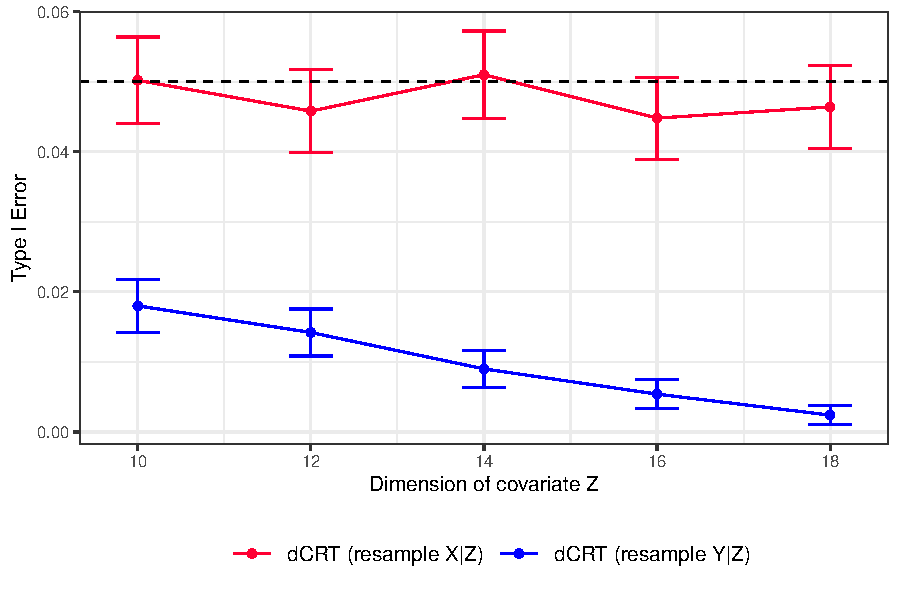
\includegraphics[width=\linewidth]{Figures/asymmetry_Poisson_type_I_error.pdf}
		\caption{Comparing the Type-I errors of the $\dCRThat$ when resampling is done based on $\lawhat_n(\prx|\prz)$ or $\lawhat_n(\pry|\prz)$.}
		\label{fig:dCRT_GCM_double_poisson_type_I_err} 
	\end{figure*}

	\begin{figure*}[ht]
		% \begin{subfigure}[b]{0.95\textwidth}
		% 	\centering
		% 	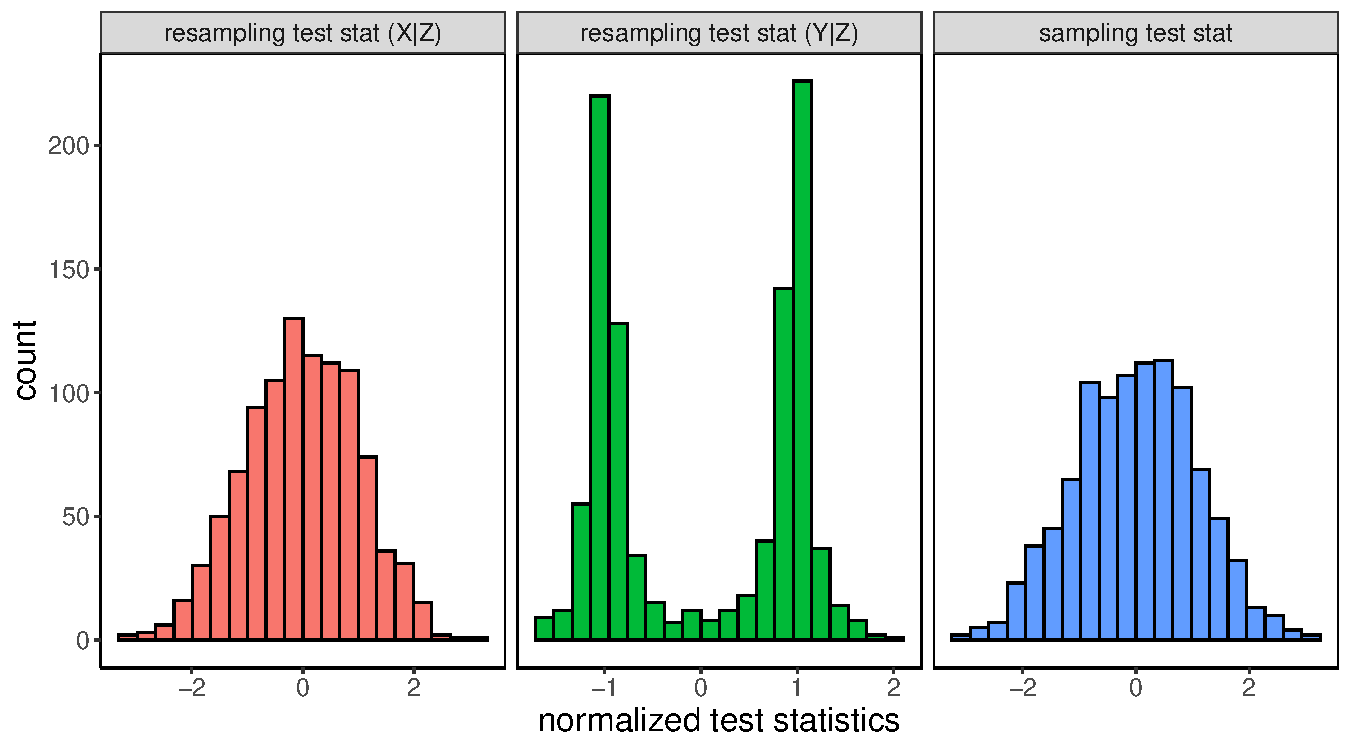
\includegraphics[width=\linewidth]{Figures/histograms_normalized.pdf} \\
		% \end{subfigure}
		\centering
			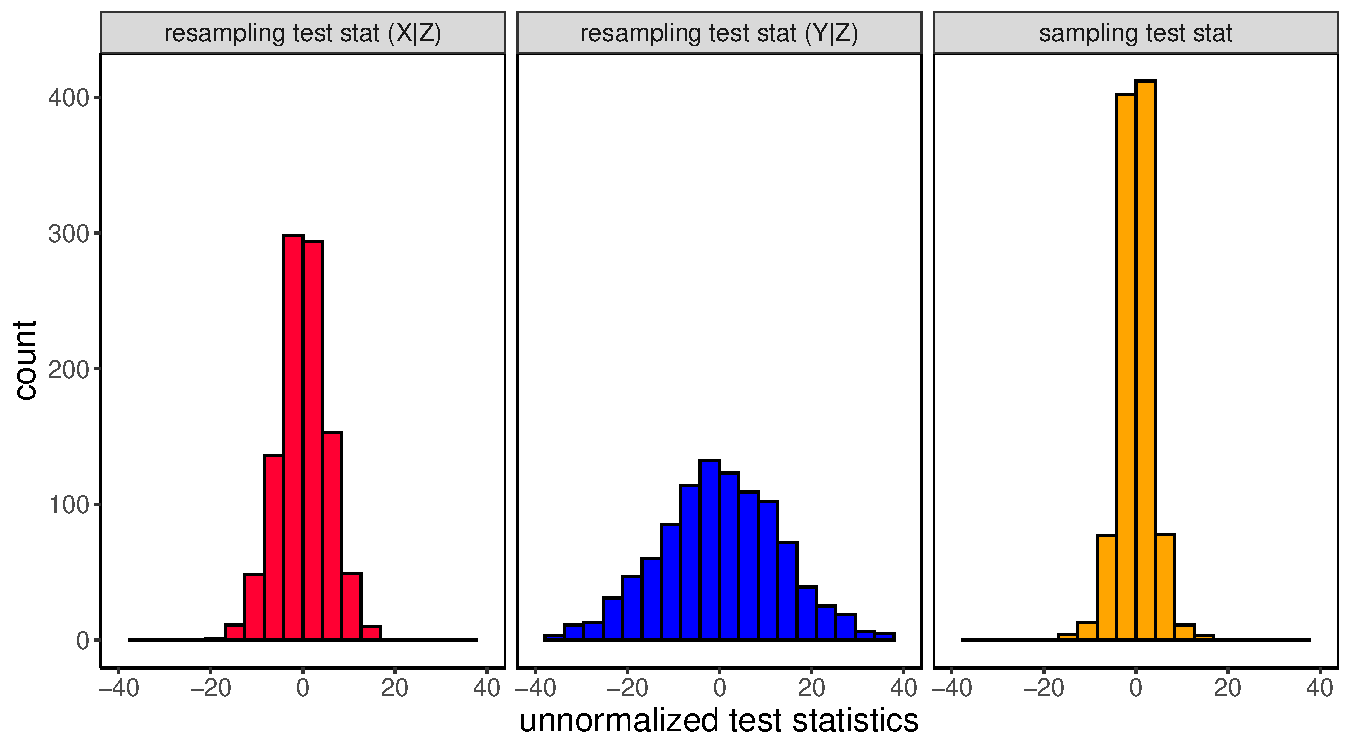
\includegraphics[width=\linewidth]{Figures/histogram_asymmetry_investigation.pdf}
		% \begin{subfigure}[b]{0.95\textwidth}
		% 	\centering
		% 	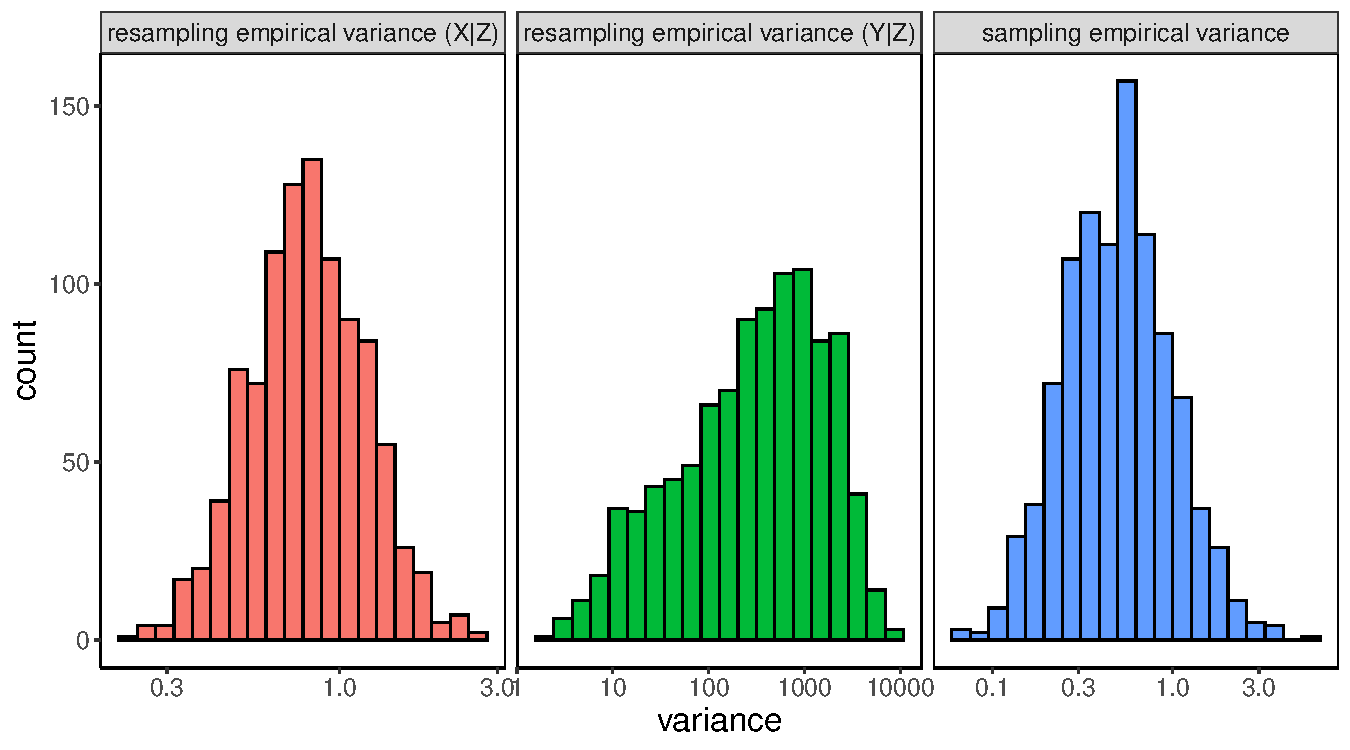
\includegraphics[width=\linewidth]{Figures/histograms_var.pdf} \\
		% \end{subfigure}
		\caption{Histograms of the resampling distributions based on resampling from $\lawhat_n(\prx|\prz)$ and $\lawhat_n(\pry|\prz)$, as well as the sampling distribution of the same statistics, in the simulation underlying Figure~\ref{fig:dCRT_GCM_double_poisson_type_I_err}.}
		\label{fig:dCRT_GCM_double_poisson_histogram} 
	\end{figure*}

	In summary, we have presented a scenario where resampling from $\lawhat_n(\prx|\prz)$ and $\lawhat_n(\pry|\prz)$ can result in different Type-I error behavior, which is due to the different levels of accuracy in these estimates. Resampling from the more accurate distribution can result in better Type-I error performance. This difference exists primarily in finite-sample regimes; as the sample size grows, both resampling strategies will converge to the GCM test under the appropriate assumptions (Theorem~\ref{thm:equivalence}). Nevertheless, this example shows that care should be taken in deciding whether to resample from $\lawhat_n(\pry|\prz)$ or $\lawhat_n(\prx|\prz)$.


	\clearpage

    %% if your bibliography is in bibtex format, uncomment commands:
    \bibliographystyle{imsart-nameyear} % Style BST file (imsart-number.bst or imsart-nameyear.bst)
    \bibliography{symcrt.bib}       % Bibliography file (usually '*.bib')



\end{document}



